\chapter{Controlling the ROV} \label{cha:controller} \index{Open-Loop Control} \index{Controller} \index{Exact Linearisation}
Automatic control is way of regulating a process without direct human interaction. This can range from approximately decoupling a dynamic system via a decoupling matrix to advanced more advanced controllers. There are two main concepts of control, open-loop and feedback control. Open-loop control is a controller that computes its output based on a model of the system and sometimes the current states. \Figureref{fig:control_system_open} illustrates the open-loop control scheme used in the \abbrROV. Feedback control is a controller that uses the error of the direct measurement or estimated state minus the reference value \textit{i.e.} 
\begin{equation}
e = \hat{x} - x_{\text{ref}}
\end{equation}
to control. The control scheme for the \abbrROV can be seen in \Figureref{fig:control_system}. A feedback controller can as the open-loop control use a model of the system. Using the model in the control structure can produce better performance and remove unwanted effects such as non-linearities, this is wanted due to the fact that a lot of control principles are based on linear systems \citep{reglerteori}. 

\begin{figure}
	\centering
		\begin{tikzpicture}[auto, thick, node distance=2cm,>=latex',
			 block/.style  = {draw, rectangle,minimum height=3em, minimum width=6em},
			 sum/.style    = {draw, circle, inner sep=0pt, text width=4mm,align=center, node distance=1cm},
			 input/.style  = {coordinate},
			 output/.style = {coordinate},
			 pinstyle/.style = {pin edge={to-,thin,black}}]
			 
		    \node [input, name=input] {};
		    \node [block, right of=input, node distance=3cm] (controller) {F};
		    \node [block, right of=controller, node distance=3cm] (system) {\abbrROV};
		
		    \draw [->] (controller) -- node[name=u] {$u$} (system);
		    \node [output, right of=system] (output) {};
		
		    \draw [draw,->] (input) -- node {$u_{\text{control}}$} (controller);
		    \draw [->] (system) -- node [name=y] {$y$}(output);
		\end{tikzpicture}
	\caption{The open-loop control scheme used in the \abbrROV. The control block F can be any type of open-loop control. Notice that this is an ideal case were no disturbances affect the system.}
	\label{fig:control_system_open}
\end{figure}

\begin{figure}
	\centering
		\begin{tikzpicture}[auto, thick, node distance=2cm,>=latex',
			 block/.style  = {draw, rectangle,minimum height=3em, minimum width=6em},
			 sum/.style    = {draw, circle, inner sep=0pt, text width=4mm,align=center, node distance=1cm},
			 input/.style  = {coordinate},
			 output/.style = {coordinate},
			 pinstyle/.style = {pin edge={to-,thin,black}}]
			 
		    \node [input, name=input] {};
		    \node [sum, right of=input] (sum) {+};
		    \node [block, right of=sum] (controller) {F};
		    \node [block, right of=controller, node distance=3cm] (system) {\abbrROV};
		
		    \draw [->] (controller) -- node[name=u] {$u$} (system);
		    \node [output, right of=system] (output) {};
		    \node [block, below of=u] (sensorfusion) {Observer};
		
		    \draw [draw,->] (input) -- node {$x_{\text{ref}}$} (sum);
		    \draw [->] (sum) -- node {$e$} (controller);
		    \draw [->] (system) -- node [name=y] {$y$}(output);
		    \draw [->] (y) |- (sensorfusion);
		    \draw [->] (sensorfusion) -| node[pos=0.99] {$-$} 
		        node [near end] {$\hat{x}$} (sum);
		\end{tikzpicture}
	\caption{The feedback control scheme used in the \abbrROV. The controller F can be any of the controllers discussed in this chapter. The observer in the \abbrROV is the sensor fusion described in \Chapterref{cha:sensor_fusion}. Notice that this is an ideal case were no disturbances affect the system.}
	\label{fig:control_system}
\end{figure}

Exact linearisation is when the dynamics of the system are compensated by a non-linear control signal and thus can linear control principles be used \citep{reglerteori}. Using the model structure from \Chapterref{cha:modelling} and the estimated parameters from \Chapterref{cha:parameterEstimation} the exact linearisation for the \abbrROV  is defined as
\begin{equation}
f^{-1}(\etaVector,\nuVector) = \inertia \accVector^{\text{b}} + \damping(\nuVector) + \coriolis(\nuVector) + \gravity(\etaVector)
\end{equation}
where $\accVector^b$ is the commanded angular acceleration in the body-fixed frame \citep[p.451]{fossen2011}.
\todo[inline]{Write some control theory. Exact lin... Background}
%%%%%%%%%%%%%%%%%%%%%%%%%%%%%%%%%%%%%%%
\section{Open-Loop Control} \label{sec:openloop} \index{Open-Loop Control} \index{thrust allocation} \index{thruster geometry}
The open loop control of the \abbrROV consists of an static thrust allocation matrix which is
\begin{equation}
    \thrusterGeometryOnes[*] = \thrusterGeometryOnes[T](\thrusterGeometryOnes \thrusterGeometryOnes[T])^{-1}
\end{equation}
where $\thrusterGeometryOnes$ describes how the actuators effect the \abbrROV \citep{thrustallocation}. The thrust geometry matrix $\thrusterGeometryOnes$ has been derived from the thrust matrix $\thrusterGeometry$ and became 
\begin{equation*}
    \thrusterGeometryOnes = 
    \begin{bmatrix}
    0  & 0  & 1 & 1  &  0 &  0 \\
    0  & 0  & 0 & 0  &  0 & -1 \\
    -1 & -1 & 0 & 0  & -1 &  0 \\
    1  & -1 & 0 & 0  &  0 &  0 \\
    1  & 1  & 0 & 0  & -1 &  0 \\
    0  & 0  & 1 & -1 &  0 &  0 \\
    \end{bmatrix}
\end{equation*}
and thus $\thrusterGeometryOnes[*]$ is given by
\begin{equation}
\thrusterGeometryOnes= \begin{bmatrix}
0 & 0 & -0.25 & 0.5 & 0.25 & 0 \\
0 & 0 & -0.25 & -0.5 & 0.25 & 0 \\
0.5 & 0 & 0 & 0 & 0 & 0.5 \\
0.5 & 0 & 0 & 0 & 0 & -0.5 \\
0 & 0 & -0.5 & 0 & -0.5 & 0 \\
0 & -1 & 0 & 0 & 0 & 0 \\
\end{bmatrix}
\end{equation}
The static thrust allocation matrix $\thrusterGeometryOnes[*]$ is the pseudo inverse of the thrust geometry matrix $\thrusterGeometryOnes$. An approximately decoupled control is achieved when the static thrust allocation matrix is used and thus can the \abbrROV be controlled better without using any controllers. \Figureref{fig:open_control} illustrates how the control signals are allocated to the different thrusters when given an control input.

\begin{figure}
    \centering
    \begin{tikzpicture}[auto, thick, node distance=3cm, >=latex',%
        block/.style    = {draw, thick, rectangle, minimum height = 3em,%
        minimum width = 3em},%
      sum/.style      = {draw, circle, node distance = 2cm},% 
      input/.style    = {coordinate},%
      output/.style   = {coordinate} %
    ]
    \draw
    	% Drawing the blocks of first filter :
    	node at (0,0)[input, name=input1] (input1) {}
    	node [block, right of=input1] (inte1) {\thrusterGeometryOnes[*]}
    	node [output, right of=inte1] (output1) {};
        % Joining blocks. 
        % Commands \draw with options like [->] must be written individually
    	\draw[->](input1) -- node {$u_{\text{control}}$}(inte1);
     	\draw[->](inte1) -- node {$u$} (output1);
    \end{tikzpicture}
    \caption{The open-loop control allocate control signals by the thrust allocation matrix $\thrusterGeometryOnes[*]$. The static thrust allocation matrix gives an approximately decoupled control.}
    \label{fig:open_control}
\end{figure}

%%%%%%%%%%%%%%%%%%%%%%%%%%%%%%%%%%%%%%%%
\section{Angular Velocities Controller} \index{Angular Velocities Controller} \index{PI@\abbrPI!abbreviation}
\todo[inline]{Write some fluff about the rate controller}

If the angular velocities error are defined as 
\begin{equation}
\nuTildeAng = \nuVectorAng - \nuVectorAng[,_{\text{ref}}]
\end{equation}
then are the \abbrPI angular velocities controller defined as 
\begin{equation}
	\accVector^b = \begin{bmatrix} 
	\zeroCol{3} \\
	\boldsymbol{T}^{-1}_\theta(\eulerAngles)(-K_{\text{p}}*\nuTildeAng - K_{\text{i}}\int \! \nuTildeAng \, \mathrm{d}t)
	\end{bmatrix}
\end{equation}
where $K_{\text{p}}$ and $K_{\text{i}}^b$ are positive definite design matrices \citep[p. 453]{fossen2011}.
Using the exact linearisation for the angular velocities controller and open-loop control for the linear velocities, are the control signals defined as
\begin{equation}
	u_{\etaVectorAng} = f^{-1}(\etaVector,\nuVector) + \thrusterGeometryOnes[*] \begin{bmatrix} \nuVectorLin \\ \zeroCol{3} \end{bmatrix}	
\end{equation}
or the control signals can be defined as 
\begin{equation}
	u_{\etaVectorAng} = \accVector^b + \thrusterGeometryOnes[*] \begin{bmatrix} \nuVectorLin \\ \zeroCol{3} \end{bmatrix}
\end{equation}
if the exact linearisation is not wanted. \Figureref{fig:ratecontroller} illustrates how the angular velocities controller is implemented with the open-loop control of the linear velocities.
\begin{figure}
	\centering
	\begin{tikzpicture}[auto, thick, node distance=2cm, >=latex',%
        block/.style  = {draw, thick, rectangle, minimum height = 1cm,%
                           minimum width = 3em},%
        PID/.style    = {draw, thick, rectangle, minimum height = 1cm,%
                         minimum width = 0.6cm},%
        sum/.style    = {draw, circle,inner sep=0pt, text width=4mm,align=center,node distance = 1cm},%
        mux/.style    = {draw, thick, rectangle, minimum width=0.3cm,%
                        minimum height = 2cm ,fill= black!100,%
                        node distance=1cm},
        input/.style    = {coordinate},%
        output/.style   = {coordinate} %
    ]
   		\draw node at (0,0) [input] (vel_input) {};
   		\draw node [input,below of=vel_input] (ang_input) {};
   		\draw node[PID, right of=ang_input] (pid) {$\abbrPI$};
   		
   		%from input to pid
   		\draw[->] (ang_input) -- node[align=center, below] {$\nuVectorAng - \nuVectorAng[,\text{ref}]$} ($(pid.west)$);
   		\draw (pid.east) -- ++(0.5,0) node[](switch){};
   		
   		%from pid to switch and making the switch 
   		\draw (pid.east) ++(2,0.5) node[](switchup){};
   		\draw (pid.east) ++(2,-0.5) node[block, name=exactlin] {$f^{-1}(\etaVector,\nuVector)$};
   		\draw (pid.east) ++(0.8,0.5) -| (switchup);
   		\draw (pid.east) ++(0.8,-0.5) -| (exactlin.west);
   		\draw (pid.east) ++(0.5,0) -- ++(0.3,0.5);
   		\draw[->] (pid.east) ++(0.65,0.25) arc (30:-30:0.6);     		
   		
   		%Merge the switch  		
   		\draw (pid.east) ++(3,0) node[coordinate](merge){};
   		\draw (switchup) -| (merge);
   		\draw (exactlin) -| (merge);
   		
   		%Input to thrust
   		\draw node[block, right of=vel_input] (thrust) {$\thrusterGeometryOnes[*]$};
   		\draw[->] (vel_input) -- node[align=center, below] {$\nuVectorLin[,\text{ref}]$} (thrust.west);
   		
   		%To sum
   		\draw (thrust.east) ++(4,0) node[sum, name=sum] {$+$};
		\draw[->] (thrust.east) -- node[align=center, below] {$u_{\nuVectorLin}$} (sum.west);
   		\draw[->] (merge) -| node[align=center, below] {$u_{\nuVectorAng}$} (sum.south);   		   		
   		% From sum to output
   		\draw node [output, right of=sum, node distance=2cm] (output) {};
    		\draw[->] (sum.east) -- node[align=center, below] {$u$} (output);
	\end{tikzpicture}
    \caption{The linear velocities are controlled in the same way as in \Sectionref{sec:openloop}. However, the angular velocities are controlled via an \abbrPID and exact linearisation can be enabled.} 
    \label{fig:ratecontroller}
\end{figure}

%%%%%%%%%%%%%%%%%%%%%%%%%%%%%%%%%%%%%%%%
\section{Attitude Controller} \index{PID@\abbrPID!abbreviation} \index{Attitude Controller}
Using the relations in \Chapterref{cha:modelling} the derivative of the attitude error can be defined as 
\begin{equation}
\etaTildeAngdot = \dot{\boldsymbol{T}}_\theta(\eulerAngles)\etaVectorAng
\end{equation}
and the attitude error can be defined as 
\begin{equation}
\etaTildeAng = \etaVectorAng - \etaVectorAng[,_{\text{ref}}] 
\end{equation}
This gives the \abbrPID attitude controller
\begin{equation}
	\accVector^b = \begin{bmatrix} 
	\zeroCol{3} \\
	\boldsymbol{T}^{-1}_\theta(\eulerAngles)(-K_{\text{p}} \etaTildeAng - K_{\text{i}}\int \! \etaTildeAng \, \mathrm{d}t - K_{\text{d}} \etaTildeAngdot - \dot{\boldsymbol{T}}_\theta(\eulerAngles) \etaVectorAng)
	\end{bmatrix}
\end{equation}
where $K_{\text{p}}$, $K_{\text{i}}$ and $K_{\text{d}}$ are positive definite design matrices \citep[p. 453]{fossen2011}. 
Using the open-loop control of the linear velocities with exact linearisation of the attitude controller gives
\begin{equation}
	u_{\etaVectorAng} = f^{-1}(\etaVector,\nuVector) + \thrusterGeometryOnes[*] \begin{bmatrix} \nuVectorLin \\ \zeroCol{3} \end{bmatrix}
\end{equation}
or
\begin{equation}
	u_{\etaVectorAng} = \accVector^b + \thrusterGeometryOnes[*] \begin{bmatrix} \nuVectorLin \\ \zeroCol{3} \end{bmatrix}
\end{equation}
without the exact linearisation. An illustration of how the attitude controller with open-loop control is implemented can be seen in \Figureref{fig:attitudecontroller}.

\begin{figure}
	\centering
	\begin{tikzpicture}[auto, thick, node distance=2cm, >=latex',%
        block/.style  = {draw, thick, rectangle, minimum height = 1cm,%
                           minimum width = 3em},%
        PID/.style    = {draw, thick, rectangle, minimum height = 1cm,%
                         minimum width = 0.6cm},%
        sum/.style    = {draw, circle,inner sep=0pt, text width=4mm,align=center,node distance = 1cm},%
        mux/.style    = {draw, thick, rectangle, minimum width=0.3cm,%
                        minimum height = 2cm ,fill= black!100,%
                        node distance=1cm},
        input/.style    = {coordinate},%
        output/.style   = {coordinate} %
    ]
   		\draw node at (0,0) [input] (vel_input) {};
   		\draw node [input,below of=vel_input] (ang_input) {};
   		\draw node[PID, right of=ang_input] (pid) {$\abbrPID$};
   		
   		%from input to pid
   		\draw[->] (ang_input) -- node[align=center, below] {$\etaVectorAng - \etaVectorAng[,\text{ref}]$} ($(pid.west)$);
   		\draw (pid.east) -- ++(0.5,0) node[](switch){};
   		
   		%from pid to switch and making the switch 
   		\draw (pid.east) ++(2,0.5) node[](switchup){};
   		\draw (pid.east) ++(2,-0.5) node[block, name=exactlin] {$f^{-1}(\etaVector,\nuVector)$};
   		\draw (pid.east) ++(0.8,0.5) -| (switchup);
   		\draw (pid.east) ++(0.8,-0.5) -| (exactlin.west);
   		\draw (pid.east) ++(0.5,0) -- ++(0.3,0.5);
   		\draw[->] (pid.east) ++(0.65,0.25) arc (30:-30:0.6);     		
   		
   		%Merge the switch  		
   		\draw (pid.east) ++(3,0) node[coordinate](merge){};
   		\draw (switchup) -| (merge);
   		\draw (exactlin) -| (merge);
   		
   		%Input to thrust
   		\draw node[block, right of=vel_input] (thrust) {$\thrusterGeometryOnes[*]$};
   		\draw[->] (vel_input) -- node[align=center, below] {$\nuVectorLin[,\text{ref}]$} (thrust.west);
   		
   		%To sum
   		\draw (thrust.east) ++(4,0) node[sum, name=sum] {$+$};
		\draw[->] (thrust.east) -- node[align=center, below] {$u_{\nuVectorLin}$} (sum.west);
   		\draw[->] (merge) -| node[align=center, below] {$u_{\etaVectorAng}$} (sum.south);   		   		
   		% From sum to output
   		\draw node [output, right of=sum, node distance=2cm] (output) {};
    		\draw[->] (sum.east) -- node[align=center, below] {$u$} (output);	
	\end{tikzpicture}
    \caption{The linear velocities are controlled in the same way as in \Sectionref{sec:openloop}. However, the attitude are controlled via an \abbrPID and exact linearisation can be enabled.} 
    \label{fig:attitudecontroller}
\end{figure}

%%%%%%%%%%%%%%%%%%%%%%%%%%%%%%%%%%%%%%%%
\section{Depth Controller} \index{Depth Controller} \index{PI@\abbrPI!abbreviation}
\todo[inline]{write some fluff} 
If the error in $\zPosition$ is defined as 
\begin{equation}
\tilde{\zPosition} = \zPosition - \zPosition_{\text{ref}}
\end{equation}
then is the \abbrPI depth controller defined as
\begin{equation}
u = \thrusterGeometryOnes[*]\begin{bmatrix} \boldsymbol{R}^n_b(\eulerAngles)^T \begin{bmatrix}
0 \\
0 \\
- K_{\text{p}} \tilde{\zPosition} - K_{\text{i}}\int \! \tilde{\zPosition} \, \mathrm{d}t
\end{bmatrix} \\ \zeroCol{3}\end{bmatrix}
\end{equation}
where $K_{\text{p}}$ and $K_{\text{i}}$ are design parameters. The rotation matrix $\boldsymbol{R}^n_b(\eulerAngles)^T$ is used to make the depth controller control the depth regardless the attitude of the \abbrROV. As can be seen in \Figureref{fig:depthcontroller} the depth controller can be used even if any of the other controllers are used. This is because the depth controller only adds or subtracts control signal to those thrusters that affect the depth.

\begin{figure}
	\centering
	\begin{tikzpicture}[auto, thick, node distance=2cm, >=latex',%
        block/.style  = {draw, thick, rectangle, minimum height = 1cm,%
                           minimum width = 3em},%
        PID/.style    = {draw, thick, rectangle, minimum height = 1cm,%
                         minimum width = 0.6cm},%
        sum/.style    = {draw, circle,inner sep=0pt, text width=4mm,align=center,node distance = 1cm},%
        mux/.style    = {draw, thick, rectangle, minimum width=0.3cm,%
                        minimum height = 2cm ,fill= black!100,%
                        node distance=1cm},
        input/.style    = {coordinate},%
        output/.style   = {coordinate} %
    ]
   		\draw node at (0,0) [input] (vel_input) {};
		\draw node[input, below of=vel_input] (ang_input) {};
   		\draw node[PID, right of=ang_input] (pid) {$\abbrPI$};
   		
   		%from input to pid
   		\draw[->] (ang_input) -- node[align=center, below] {$\zPosition - \zPosition_{\text{ref}}$} ($(pid.west)$);
   		\draw (pid.east) -- ++(0.5,0) node[](switch){};
   		
   		%from pid to switch and making the switch 
   		\draw (pid.east) ++(2,0) node[coordinate](switchup){};
  		\draw (pid.east) ++(1.2,0) -- (switchup);
   		\draw (pid.east) ++(0.5,0) -- ++(0.3,0.5);
   		\draw[->] (pid.east) ++(0.65,0.25) arc (30:0:0.6);     		
   		
   		%Merge the switch  		
   		\draw (pid.east) ++(3,0) node[coordinate](merge){};
   		\draw (switchup) -- (merge);
   		
   		%Input to thrust
   		\draw node[block, right of=vel_input] (controller) {F};
   		\draw[->] (vel_input) -- node[align=center, below] {$x_{\text{ref}}$} (controller.west);
   		
   		%To sum
   		\draw (controller.east) ++(4,0) node[sum, name=sum] {$+$};
		\draw[->] (controller.east) -- (sum.west);
   		\draw[->] (merge) -| node[align=center, below] {$u_{\zPosition}$}  (sum.south);   		   		
   		% From sum to output
   		\draw node [output, right of=sum, node distance=2cm] (output) {};
    		\draw[->] (sum.east) -- node[align=center, below] {$u$} (output);
	\end{tikzpicture}
    \caption{The \abbrPI depth controller can be used when the open-loop control is engaged or when the other controllers are used. In this figure the F symbolises the chosen way of controlling the \abbrROV.} 
    \label{fig:depthcontroller}
\end{figure}

%%%%%%%%%%%%%%%%%%%%%%%%%%%%%%%%%%%%%%%%
\section{Benchmarking}
To be able to draw any conclusions about the performance of the controllers the following reference signals was used
\begin{description}
\item[Constant] A constant reference was applied to all \abbrDOF.
\item[Sine] A $\sin(\cdot)$ signal  was applied to one \abbrDOF at the time and then to all \abbrDOF. Two different $\sin$ signals were used, with amplitude {\color{red} 9999999, 1111111} and frequency {\color{red} 9999999, 11111} $\hertz$ respectively. \todo[inline]{fix amplitude and frequency}
\item[Smooth step] A smooth step was applied to one \abbrDOF at the time and then to all \abbrDOF at the same time. The used smooth step was the same as in \citet[p. 192-195]{robotics}. The smooth step parameters was $q_{\text{0}} = $, $q_{\text{f}}$, $t_{\text{s}} = $ ,$t_{\text{f}} = $ and $V = 1.5 (q_{\text{f}} - q_{\text{0}})/(t_{\text{f}} - t_{\text{s}}))$ \todo[inline]{fix parameter values}.  
\end{description}
for each controller separately.
%%%%%%%%%%%%%%%%%%%%%%%%%%%Attitude%%%%%%%%%%%%%%%%
\begin{figure}[tbp]
  \centering
  \subfloat[][\label{fig:testStepPhi} An step was applied to $\rollAngle$ .]{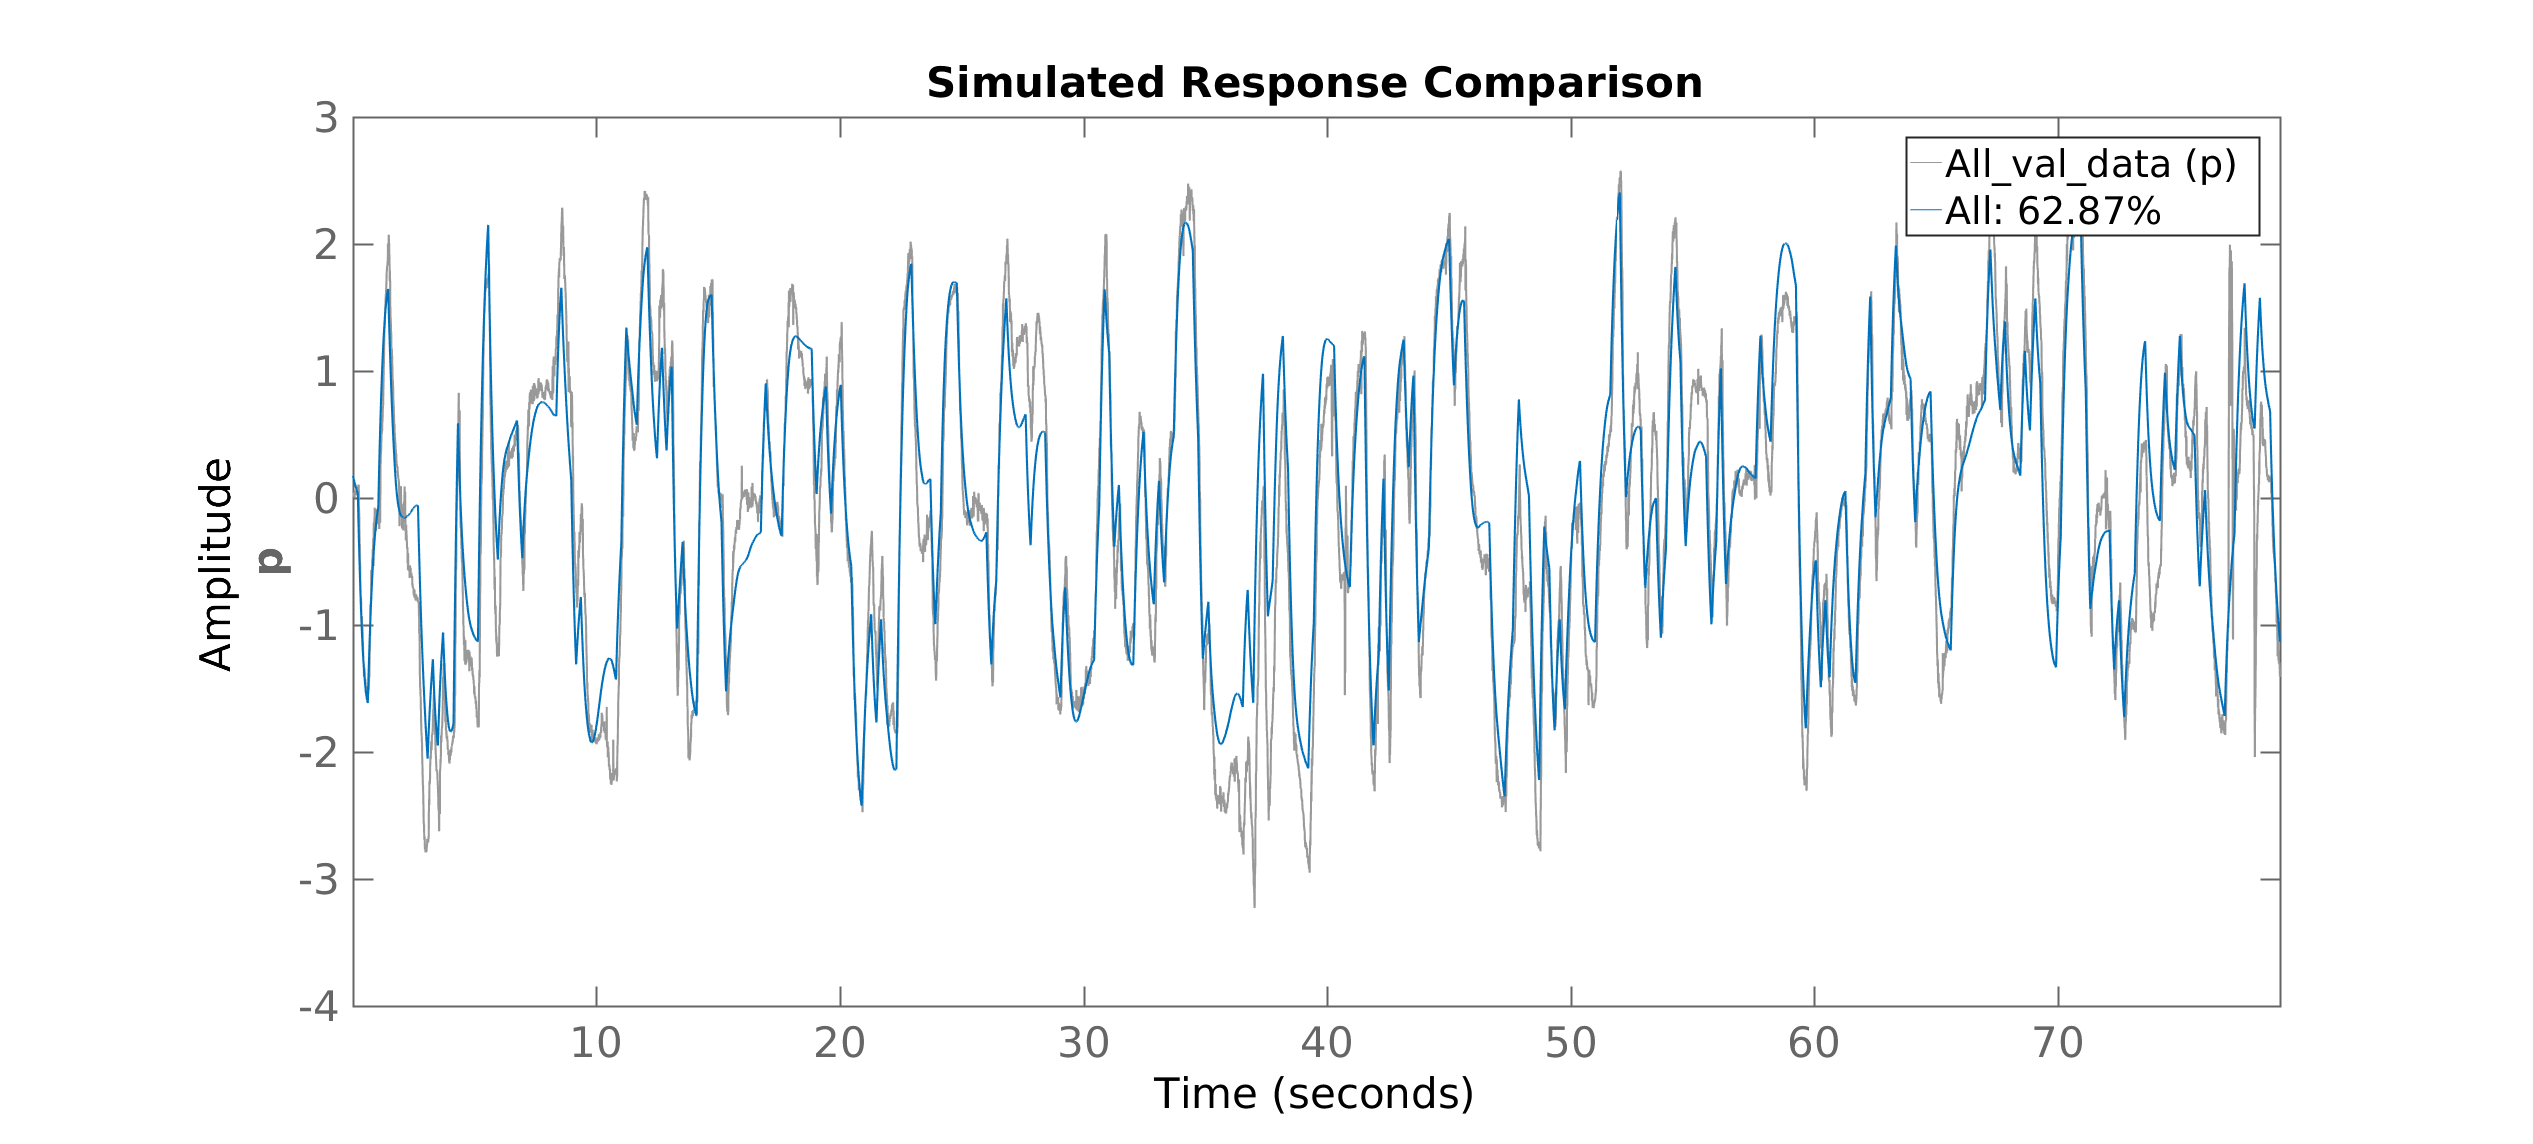
\includegraphics[width=0.4\textwidth]{velocityComparep}}
  \qquad
  \subfloat[][\label{fig:simStepPhi} An step was applied to the simulated \abbrROV in $\rollAngle$.]{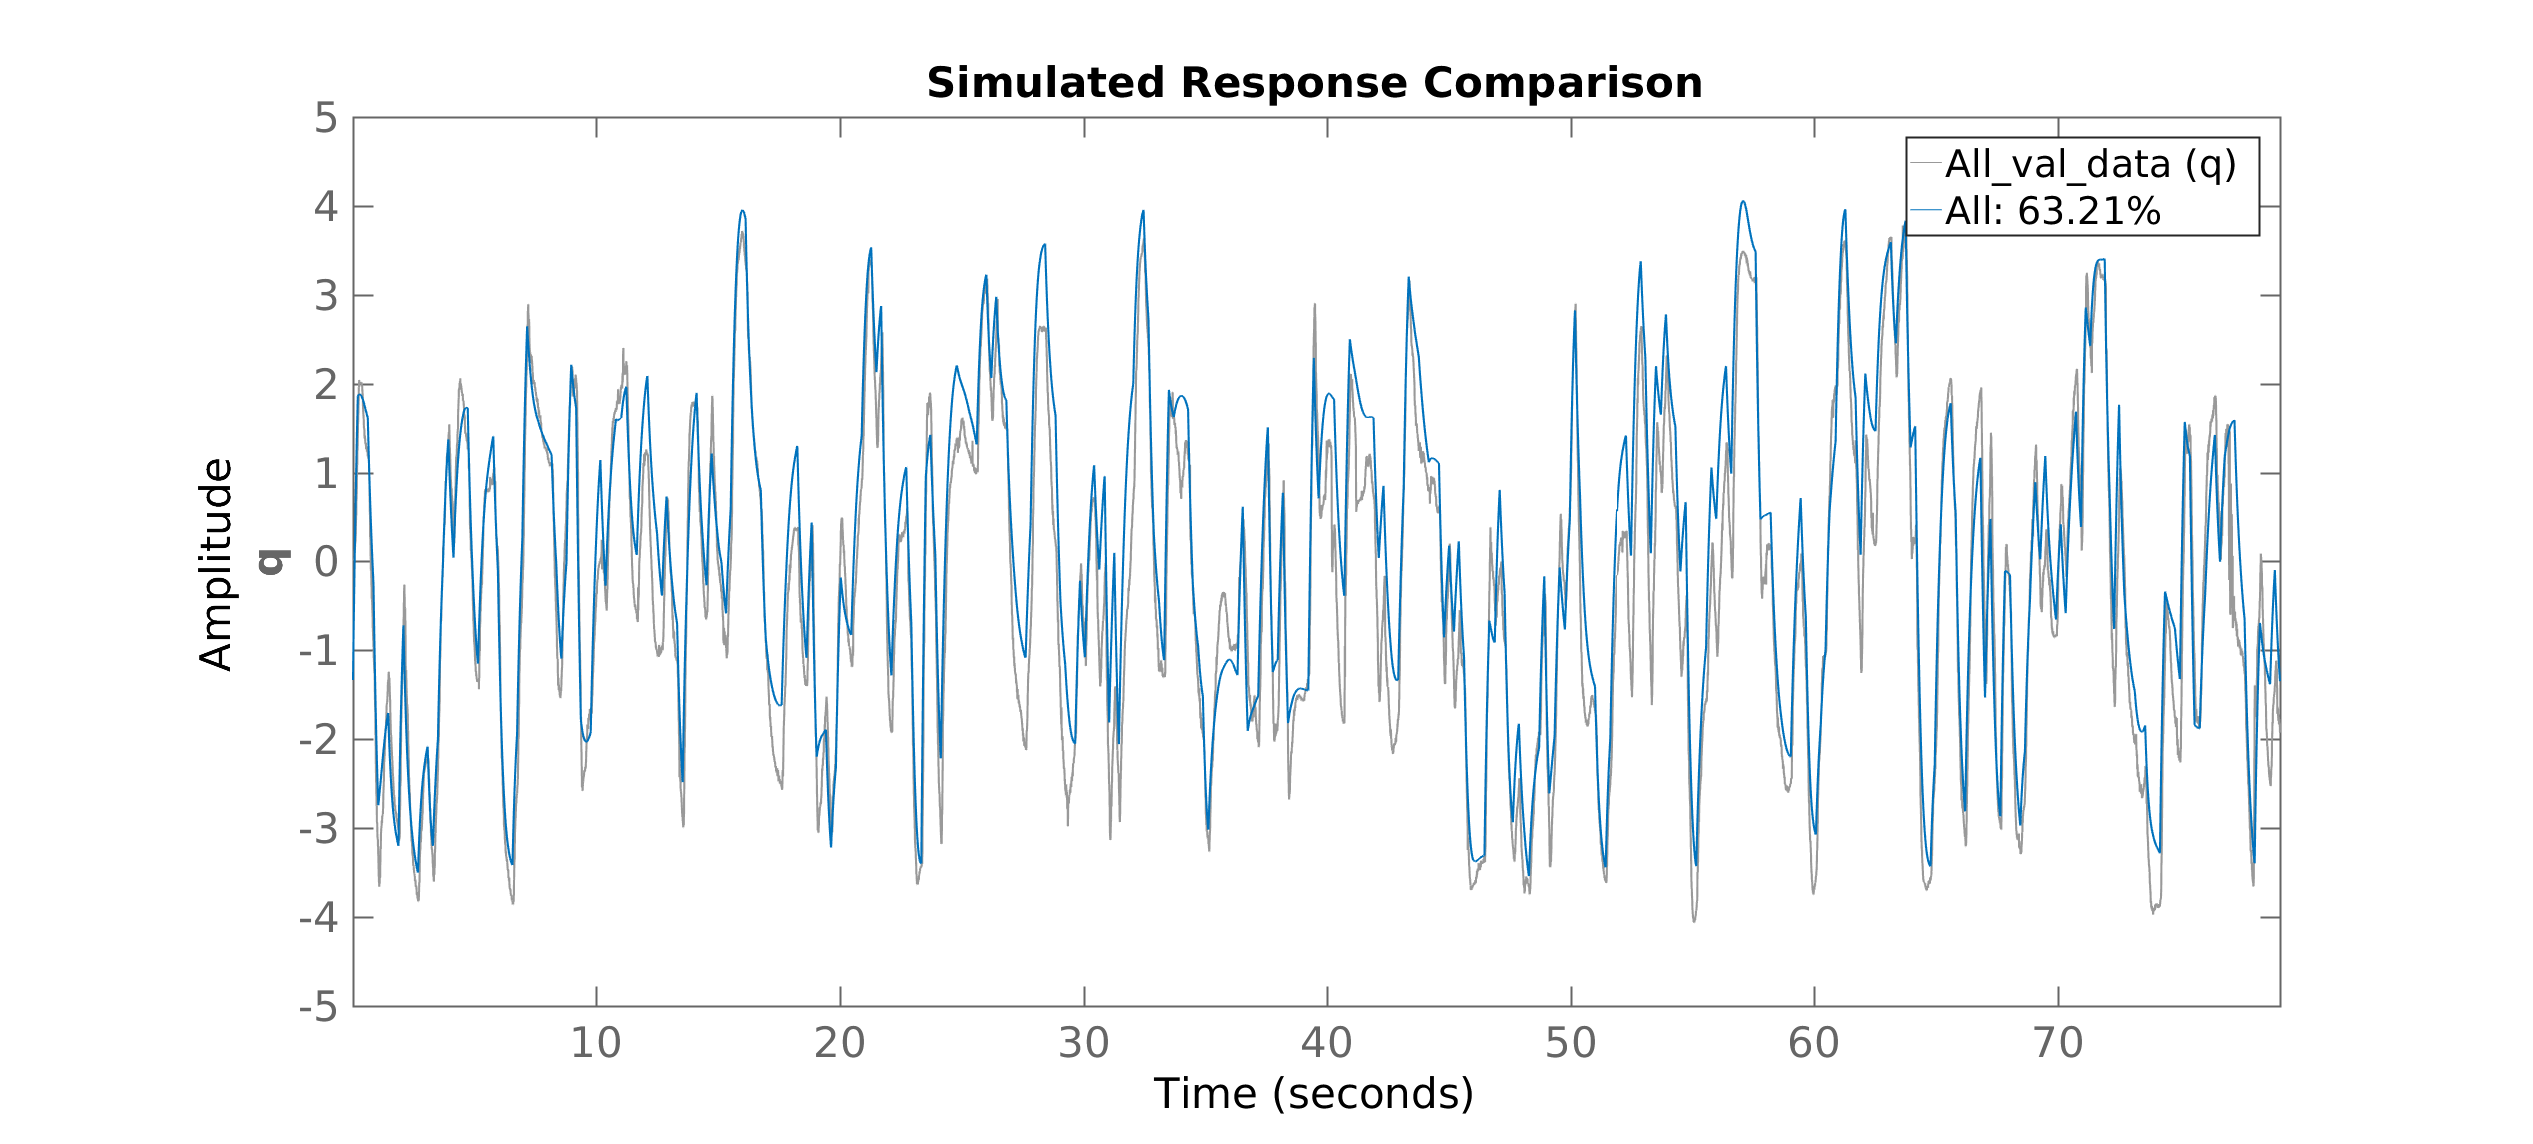
\includegraphics[width=0.4\textwidth]{velocityCompareq}}
  \qquad
  \subfloat[][\label{fig:testStepTheta} An step was applied to $\pitchAngle$ .]{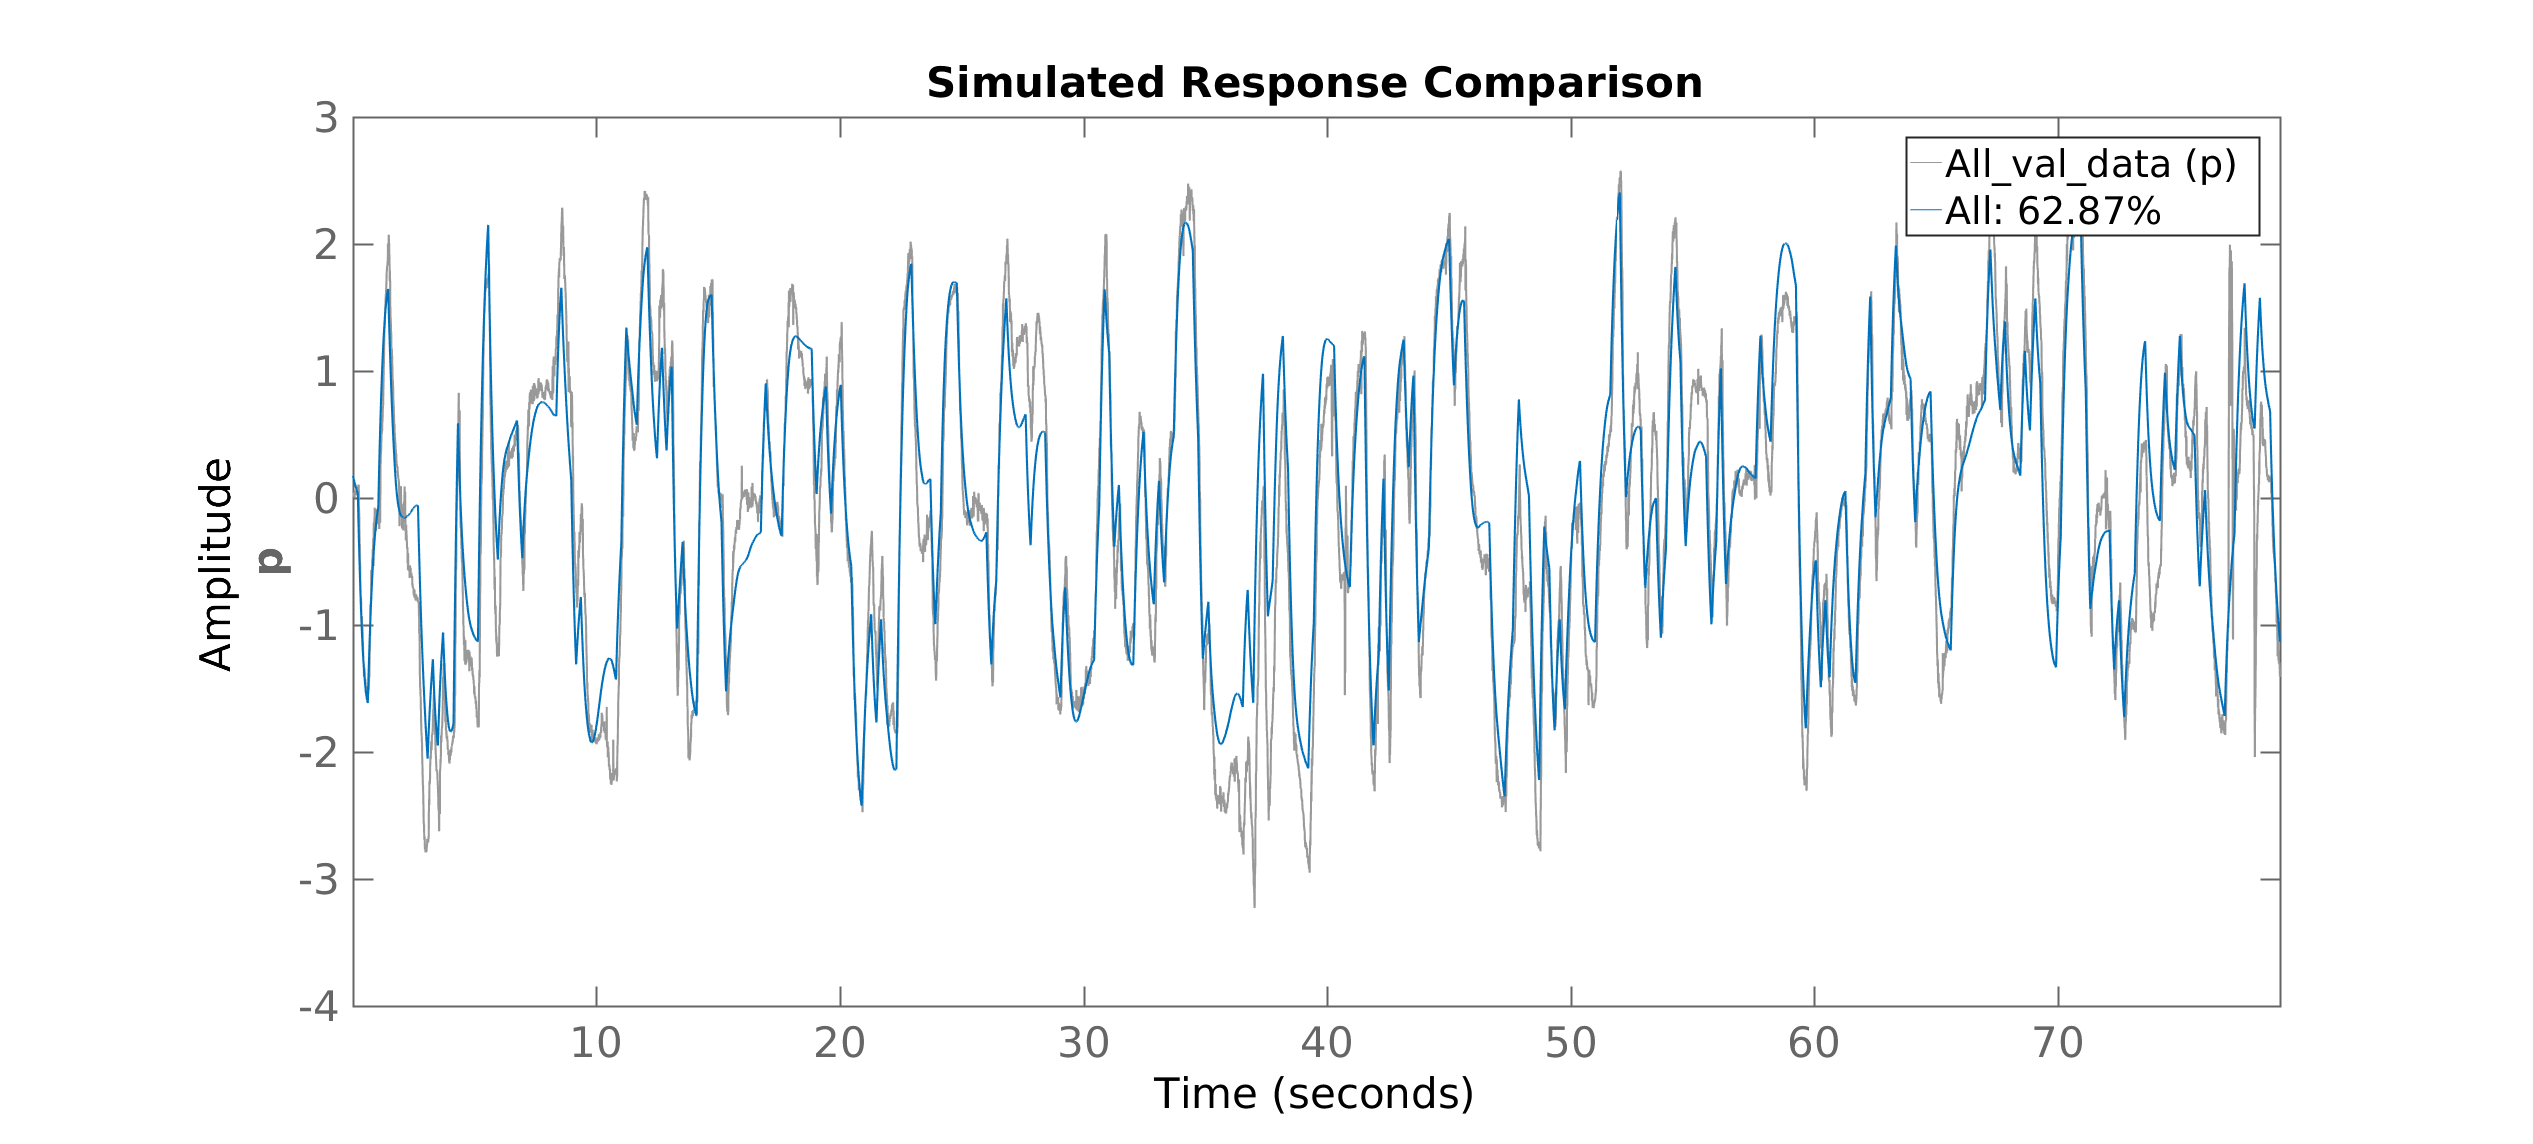
\includegraphics[width=0.4\textwidth]{velocityComparep}}
  \qquad
  \subfloat[][\label{fig:simStepTheta} An step was applied to the simulated \abbrROV in $\pitchAngle$.]{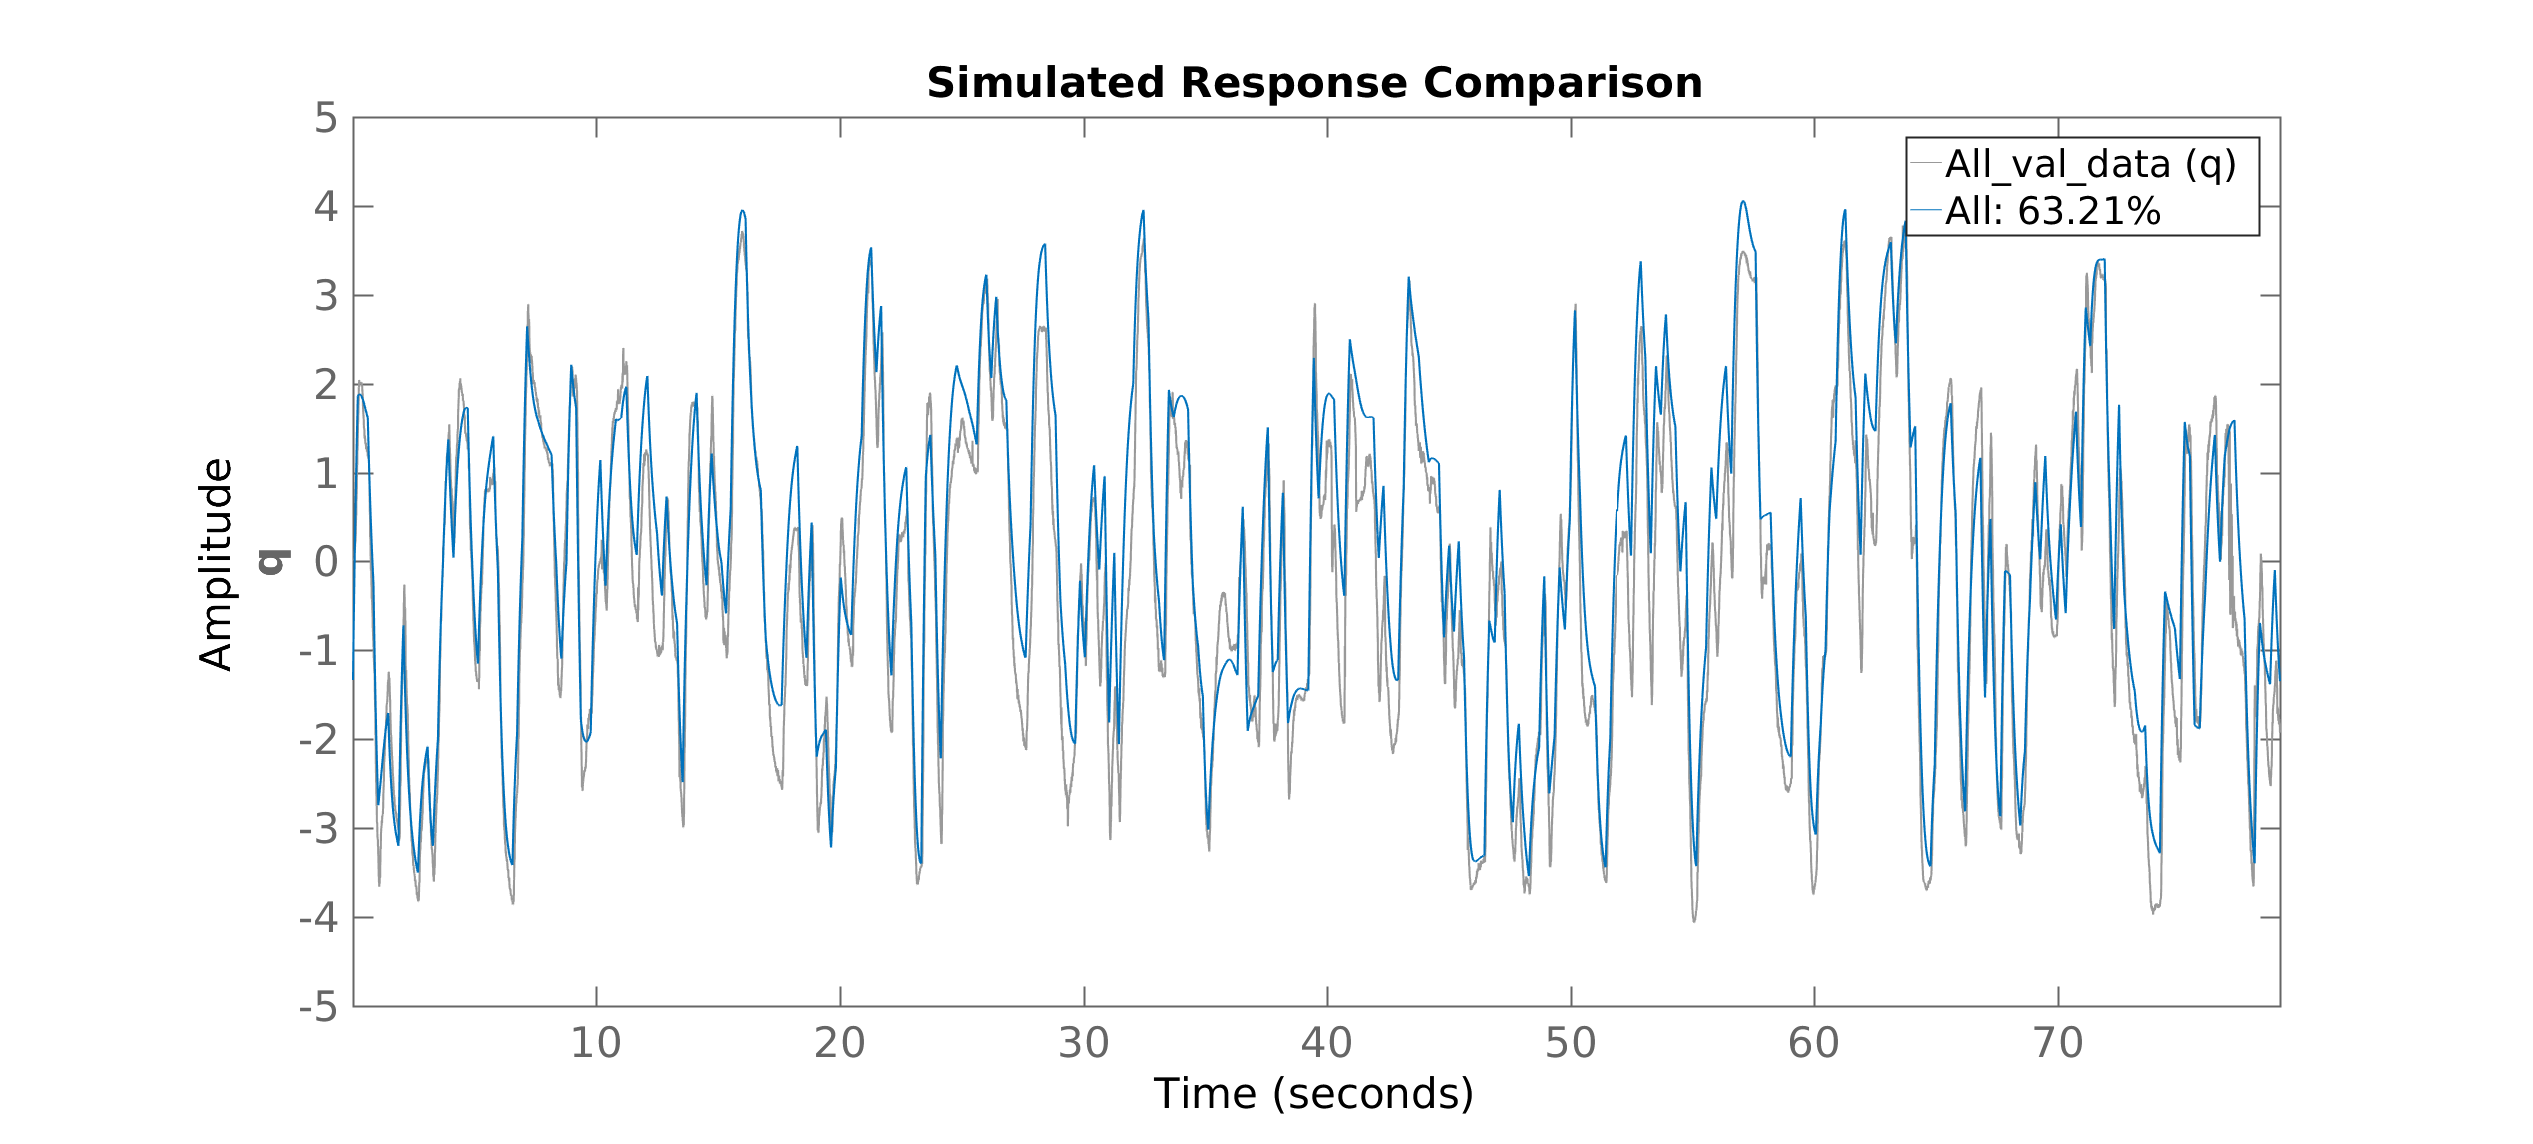
\includegraphics[width=0.4\textwidth]{velocityCompareq}}
  \qquad
  \subfloat[][\label{fig:testStepPsi} An step was applied to $\yawAngle$ .]{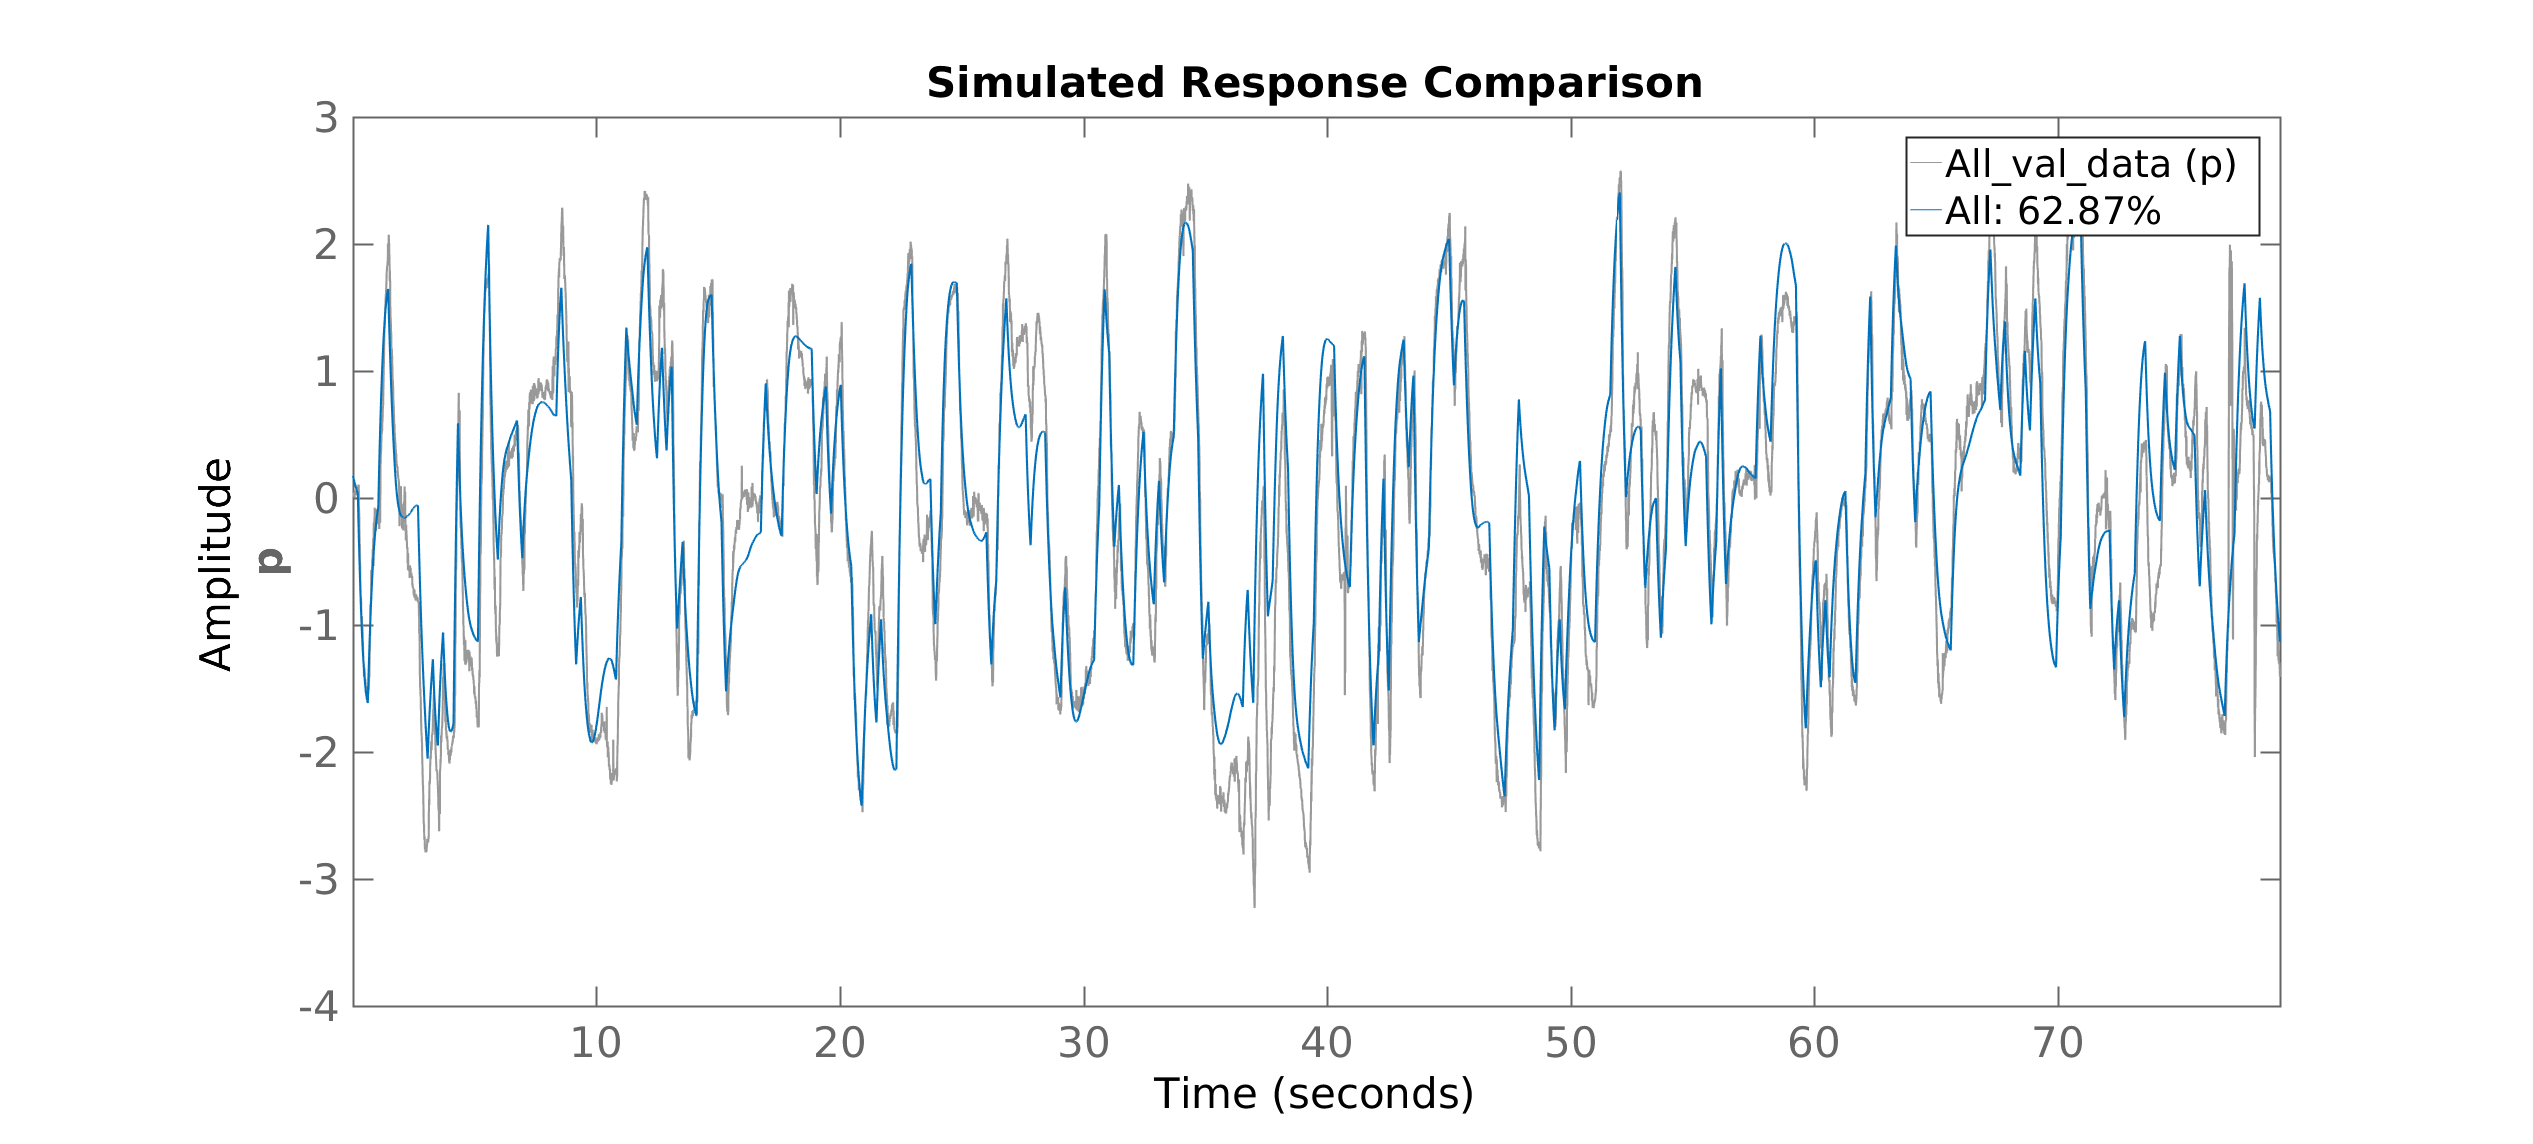
\includegraphics[width=0.4\textwidth]{velocityComparep}}
  \qquad
  \subfloat[][\label{fig:simStepPsi} An step was applied to the simulated \abbrROV in $\yawAngle$.]{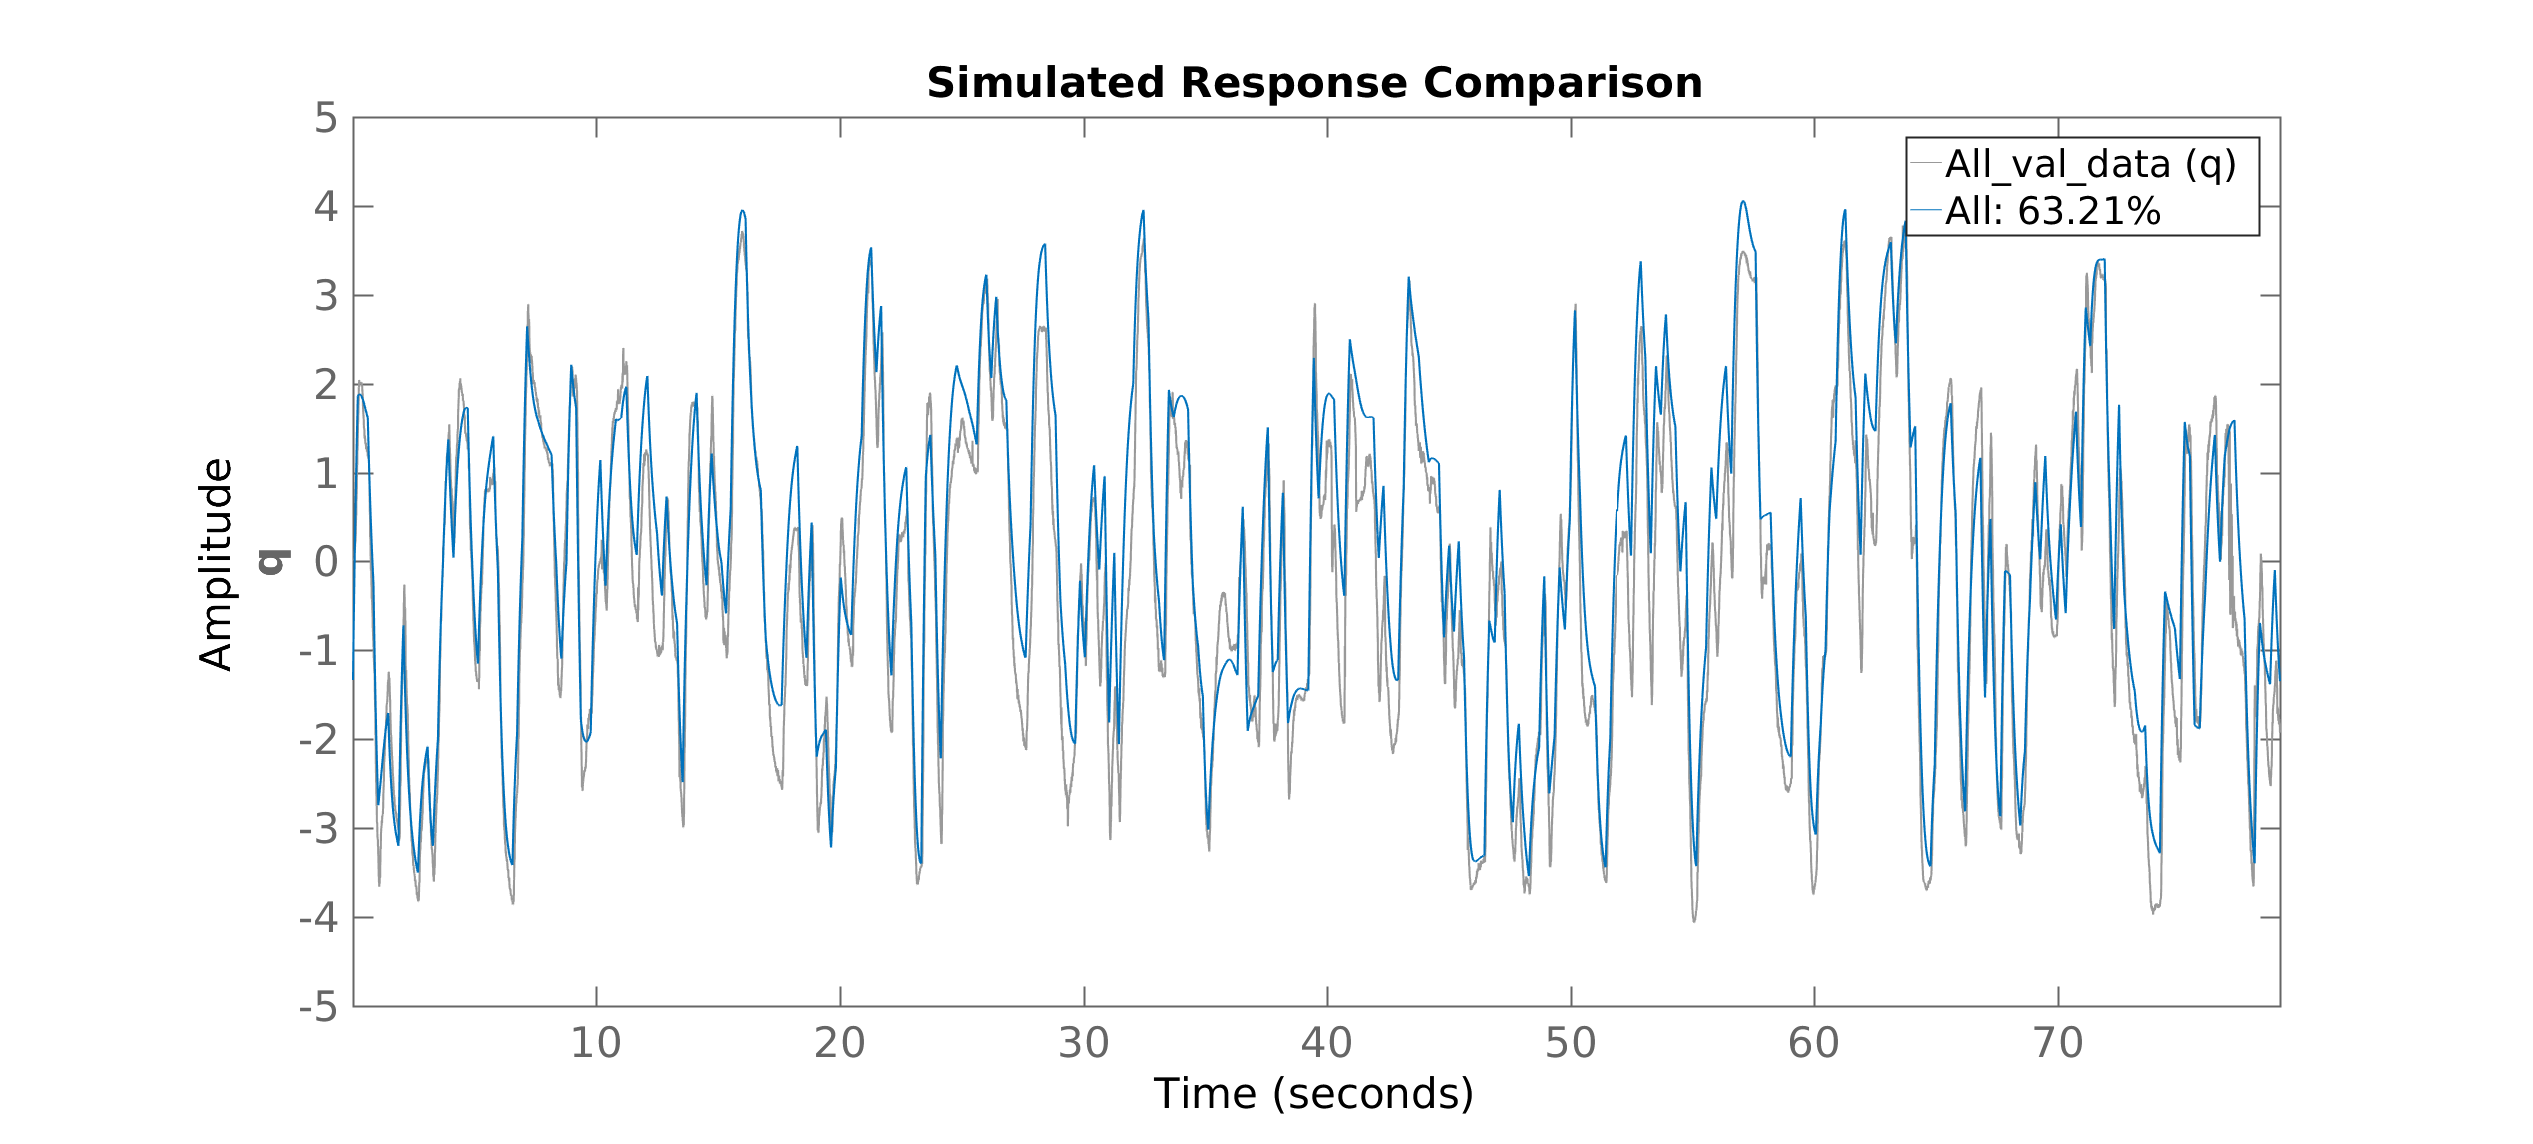
\includegraphics[width=0.4\textwidth]{velocityCompareq}}
    \qquad
  \subfloat[][\label{fig:testStepAll} An step was applied to all \abbrDOF.]{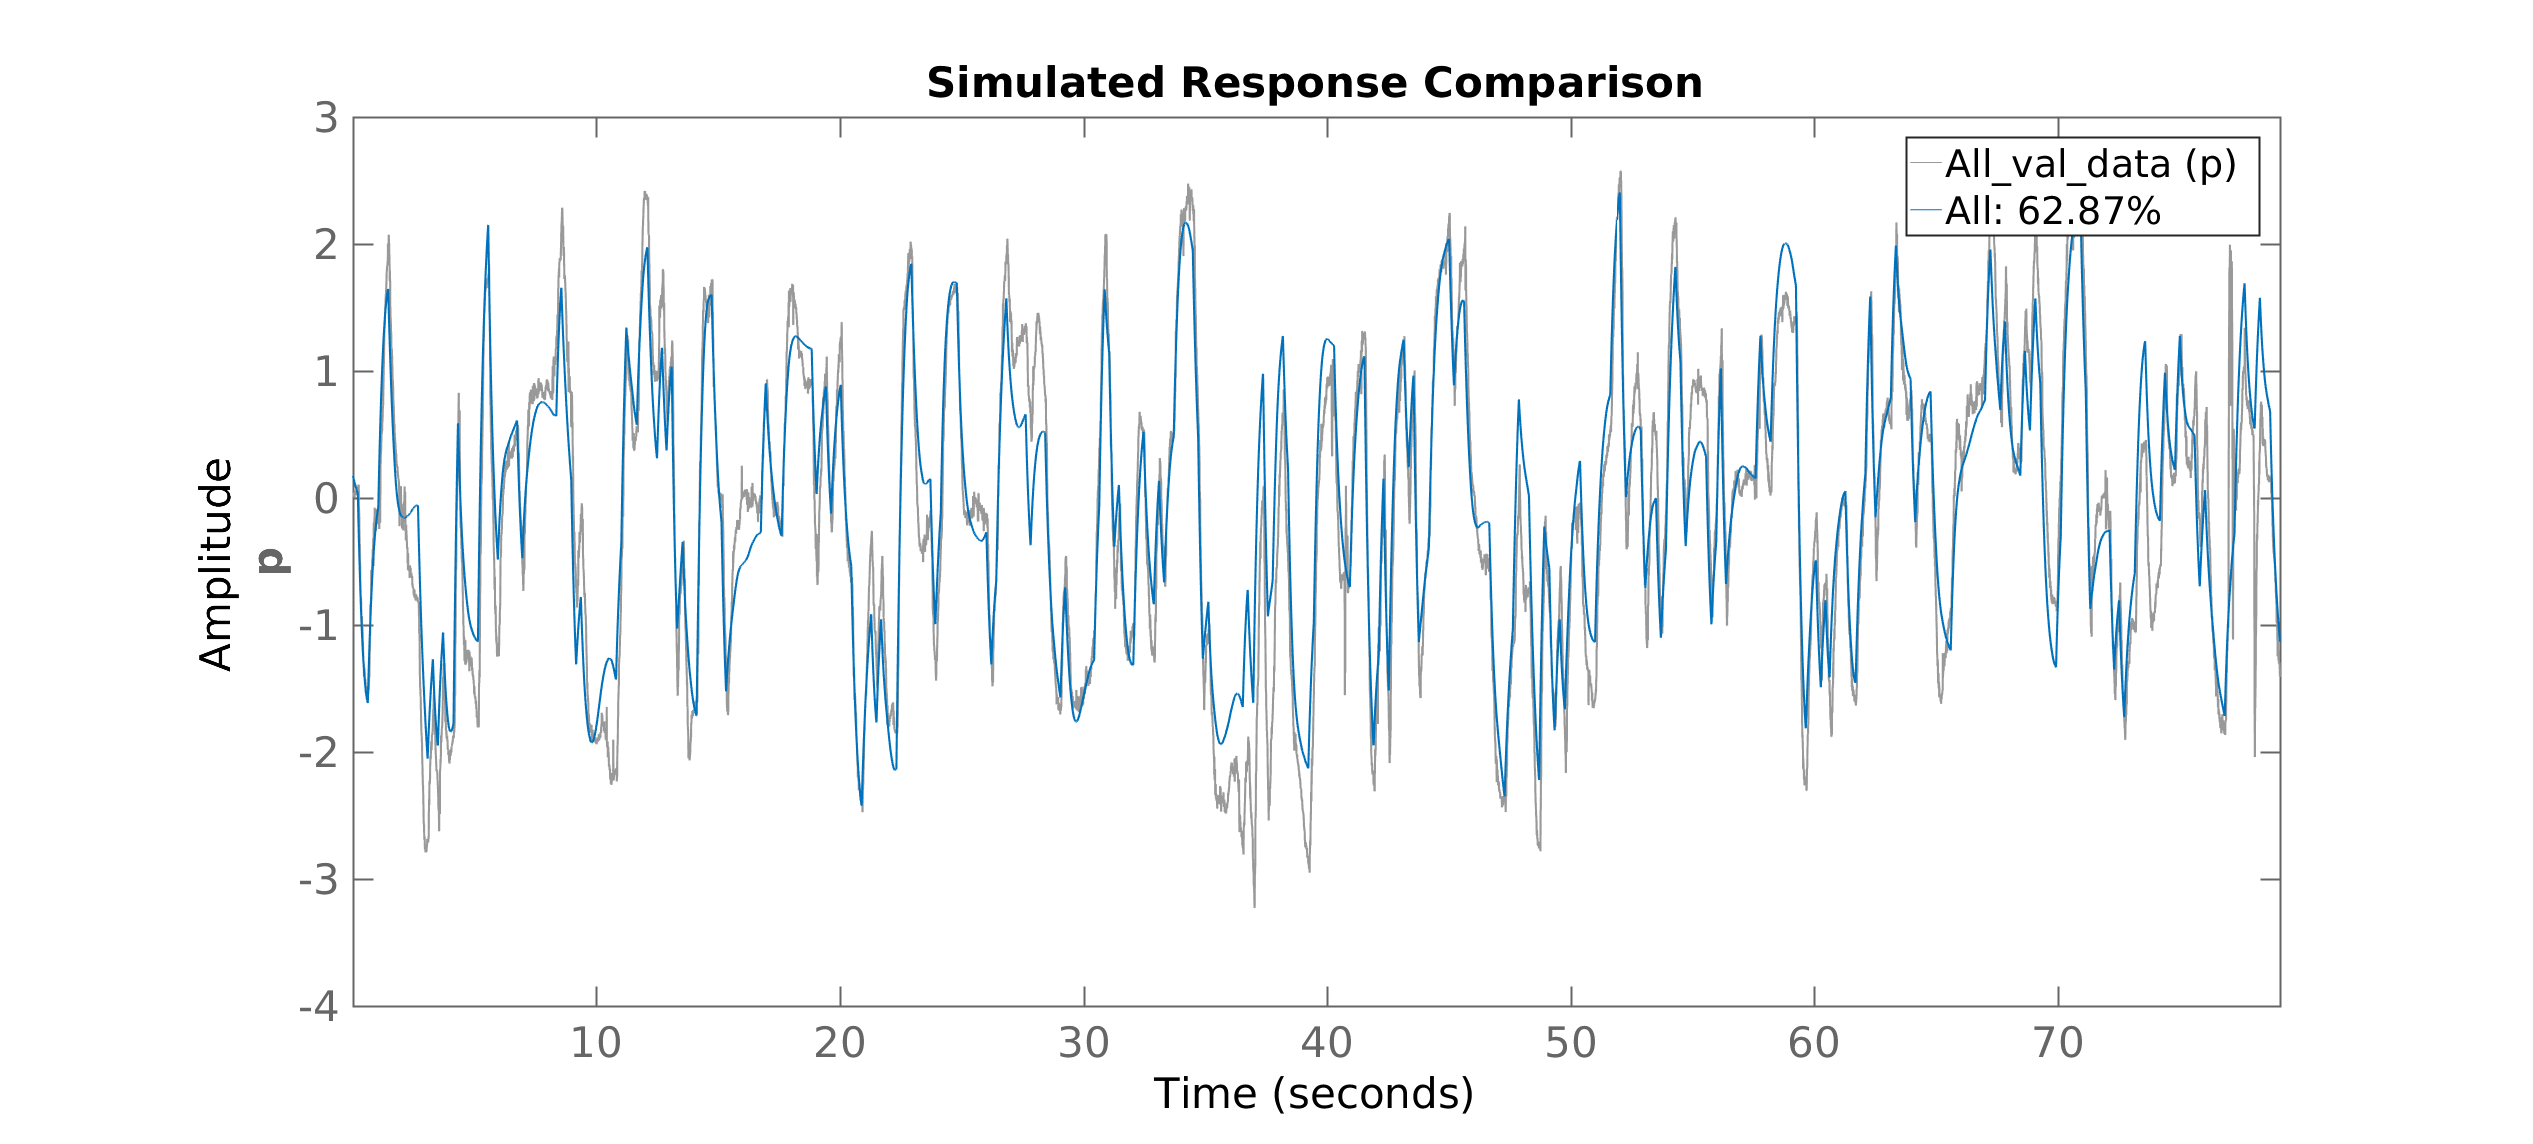
\includegraphics[width=0.4\textwidth]{velocityComparep}}
  \qquad
  \subfloat[][\label{fig:simStepAll} An step was applied to the simulated \abbrROV in all \abbrDOF.]{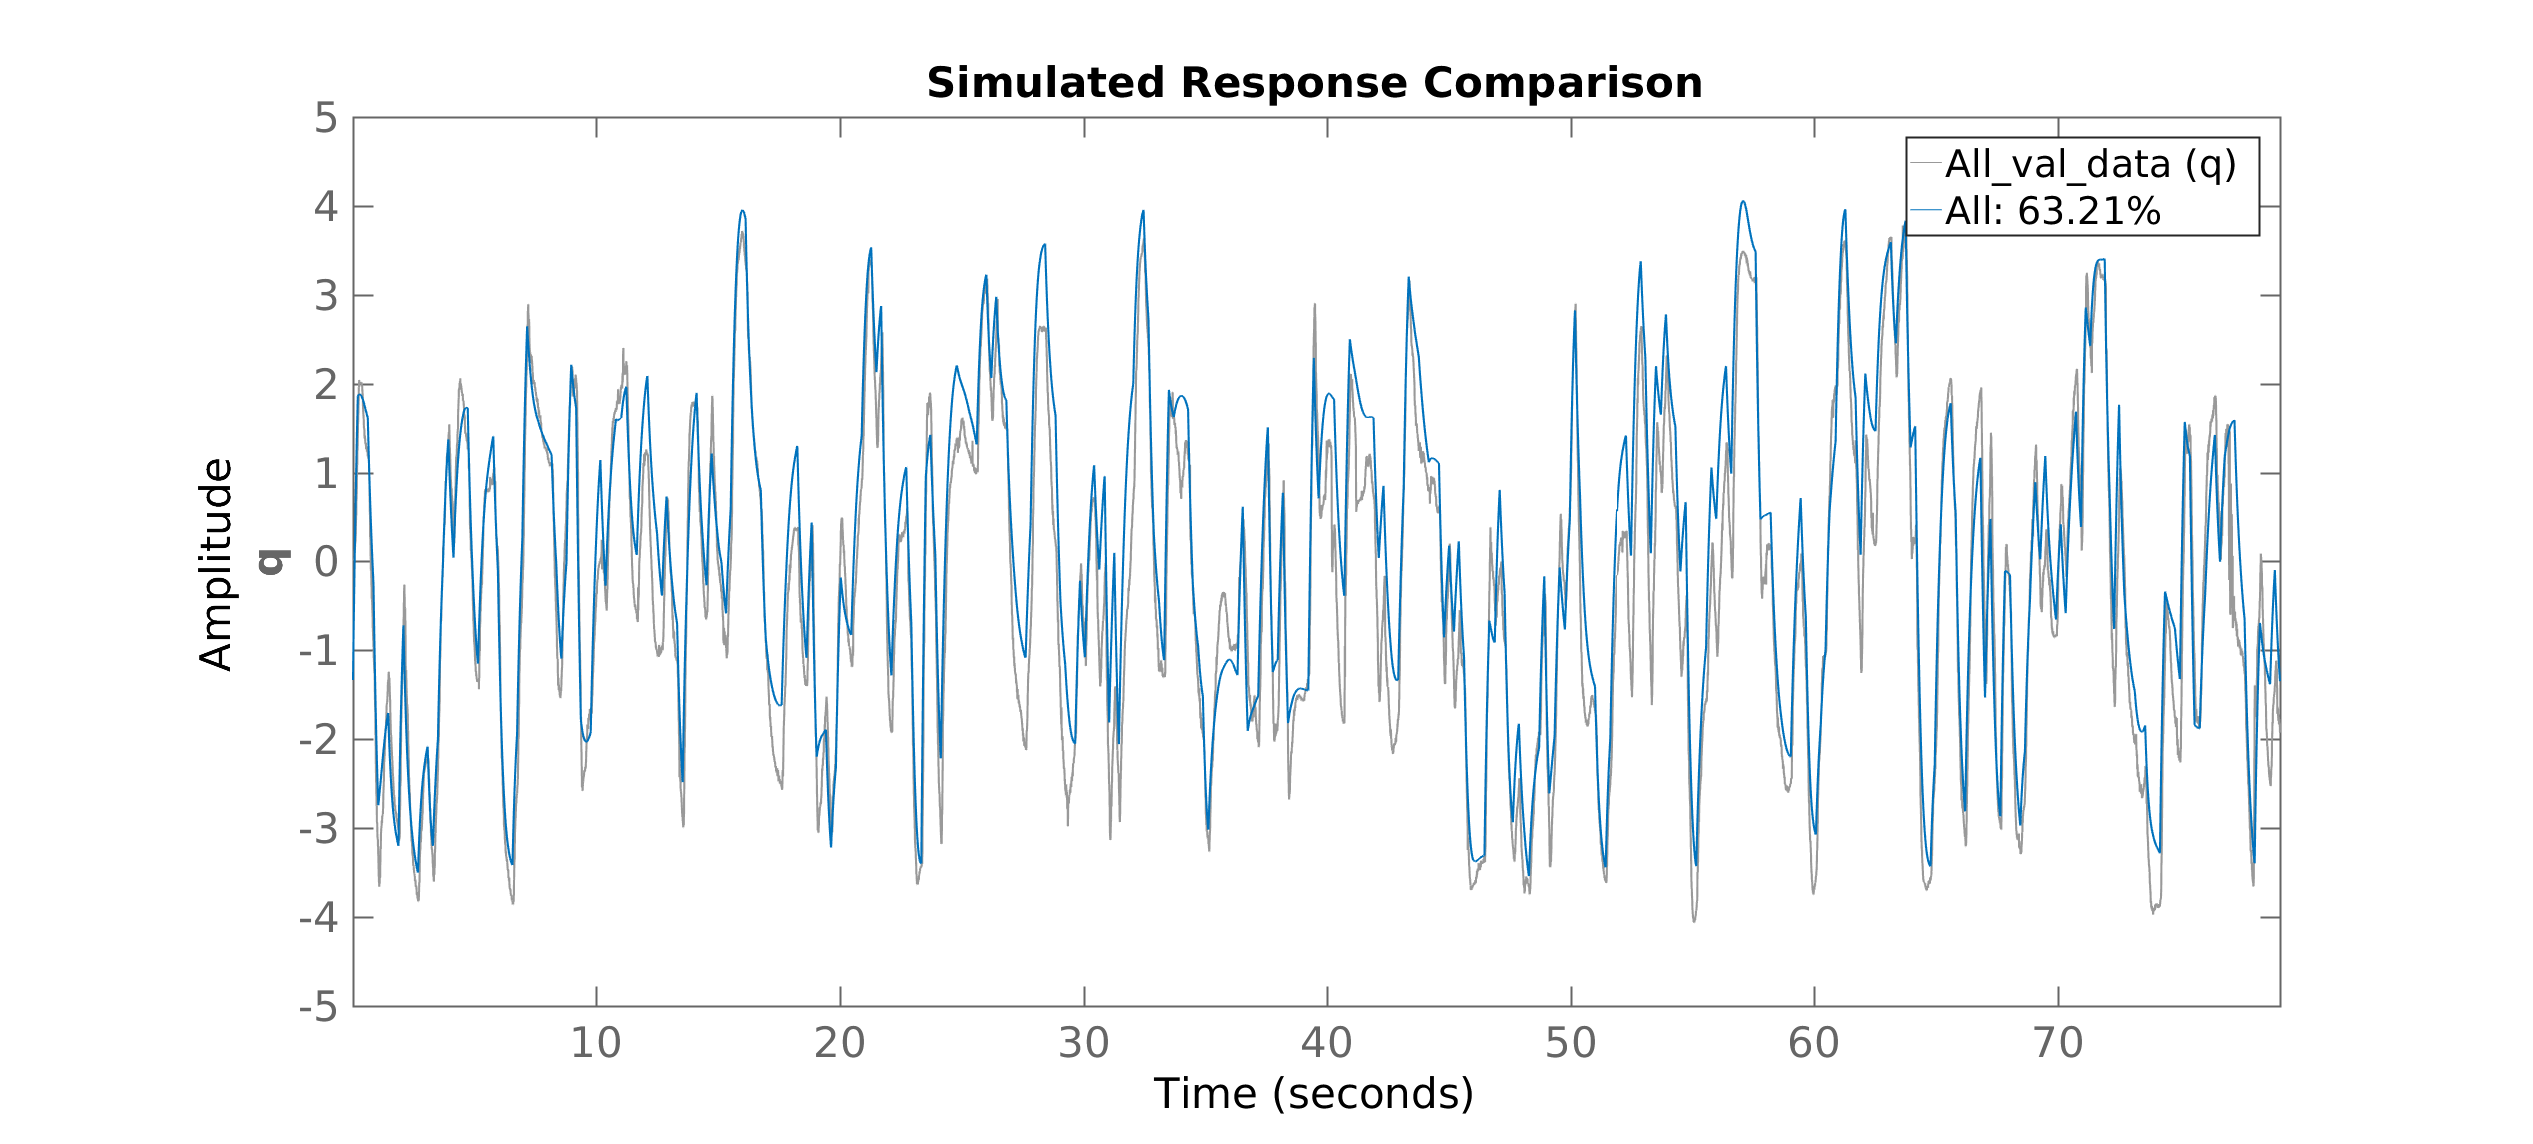
\includegraphics[width=0.4\textwidth]{velocityCompareq}}
  \caption{\label{fig:StepAttitude}%
    Comparison between simulation and a real test of a smooth step reference in.}
\end{figure}


%%%%%%%%%%%%%%%%%%%%%%%%%%%Rate%%%%%%%%%%%%%%%%
\begin{figure}[tbp]
  \centering
  \subfloat[][\label{fig:testStepP} An step was applied to $\rollVelocity$ .]{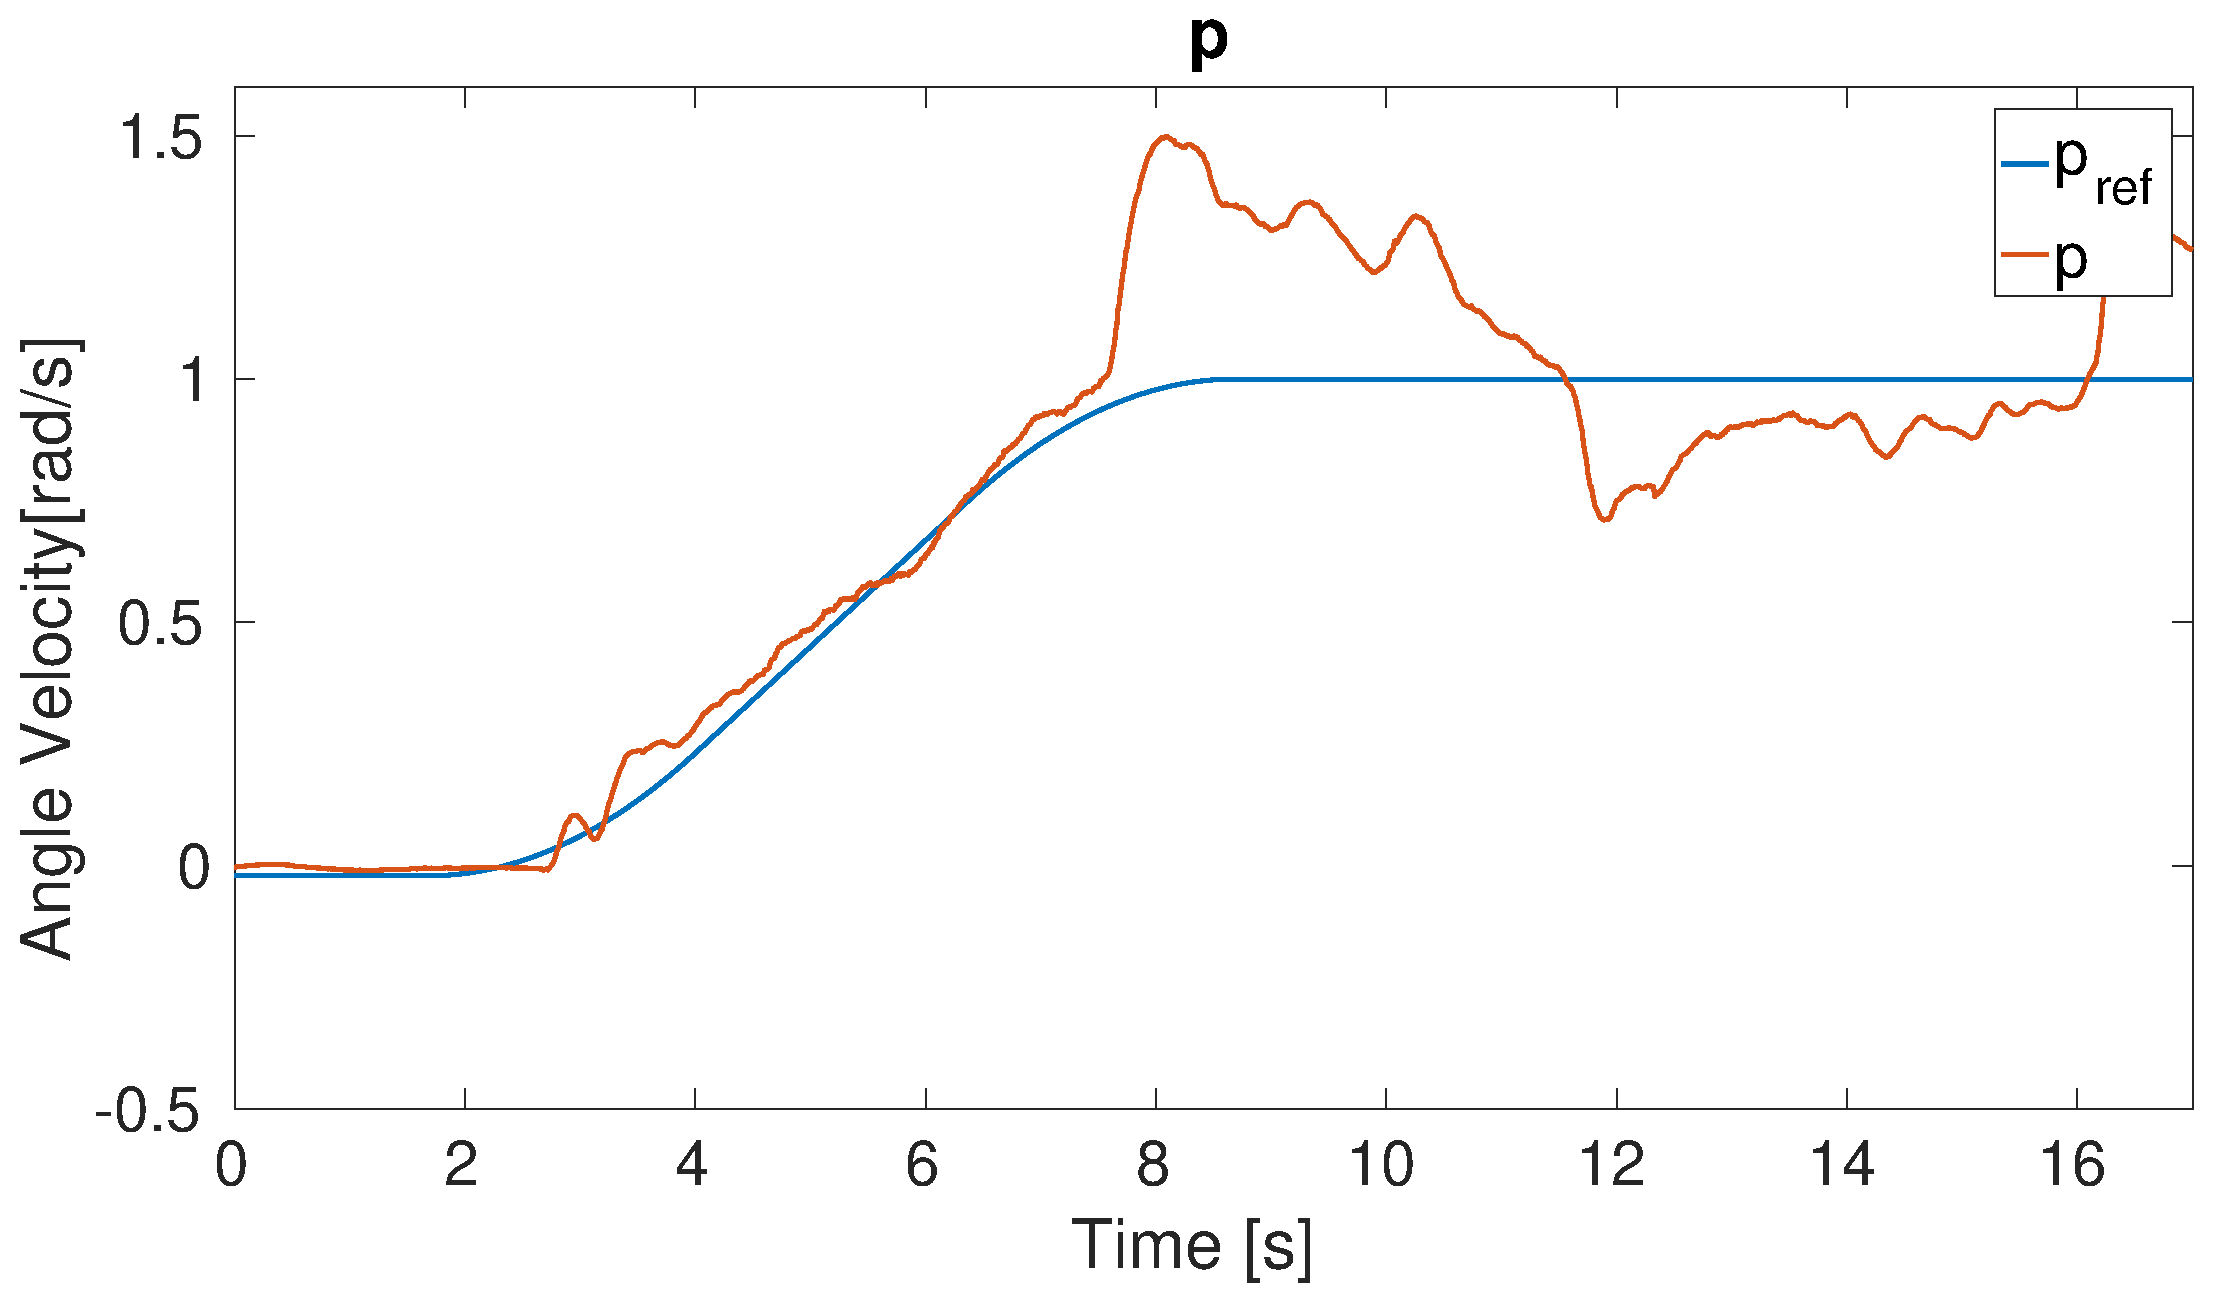
\includegraphics[width=0.4\textwidth]{testStepPs3e10a1}}
  \qquad
  \subfloat[][\label{fig:simStepP} An step was applied to the simulated \abbrROV in $\rollVelocity$.]{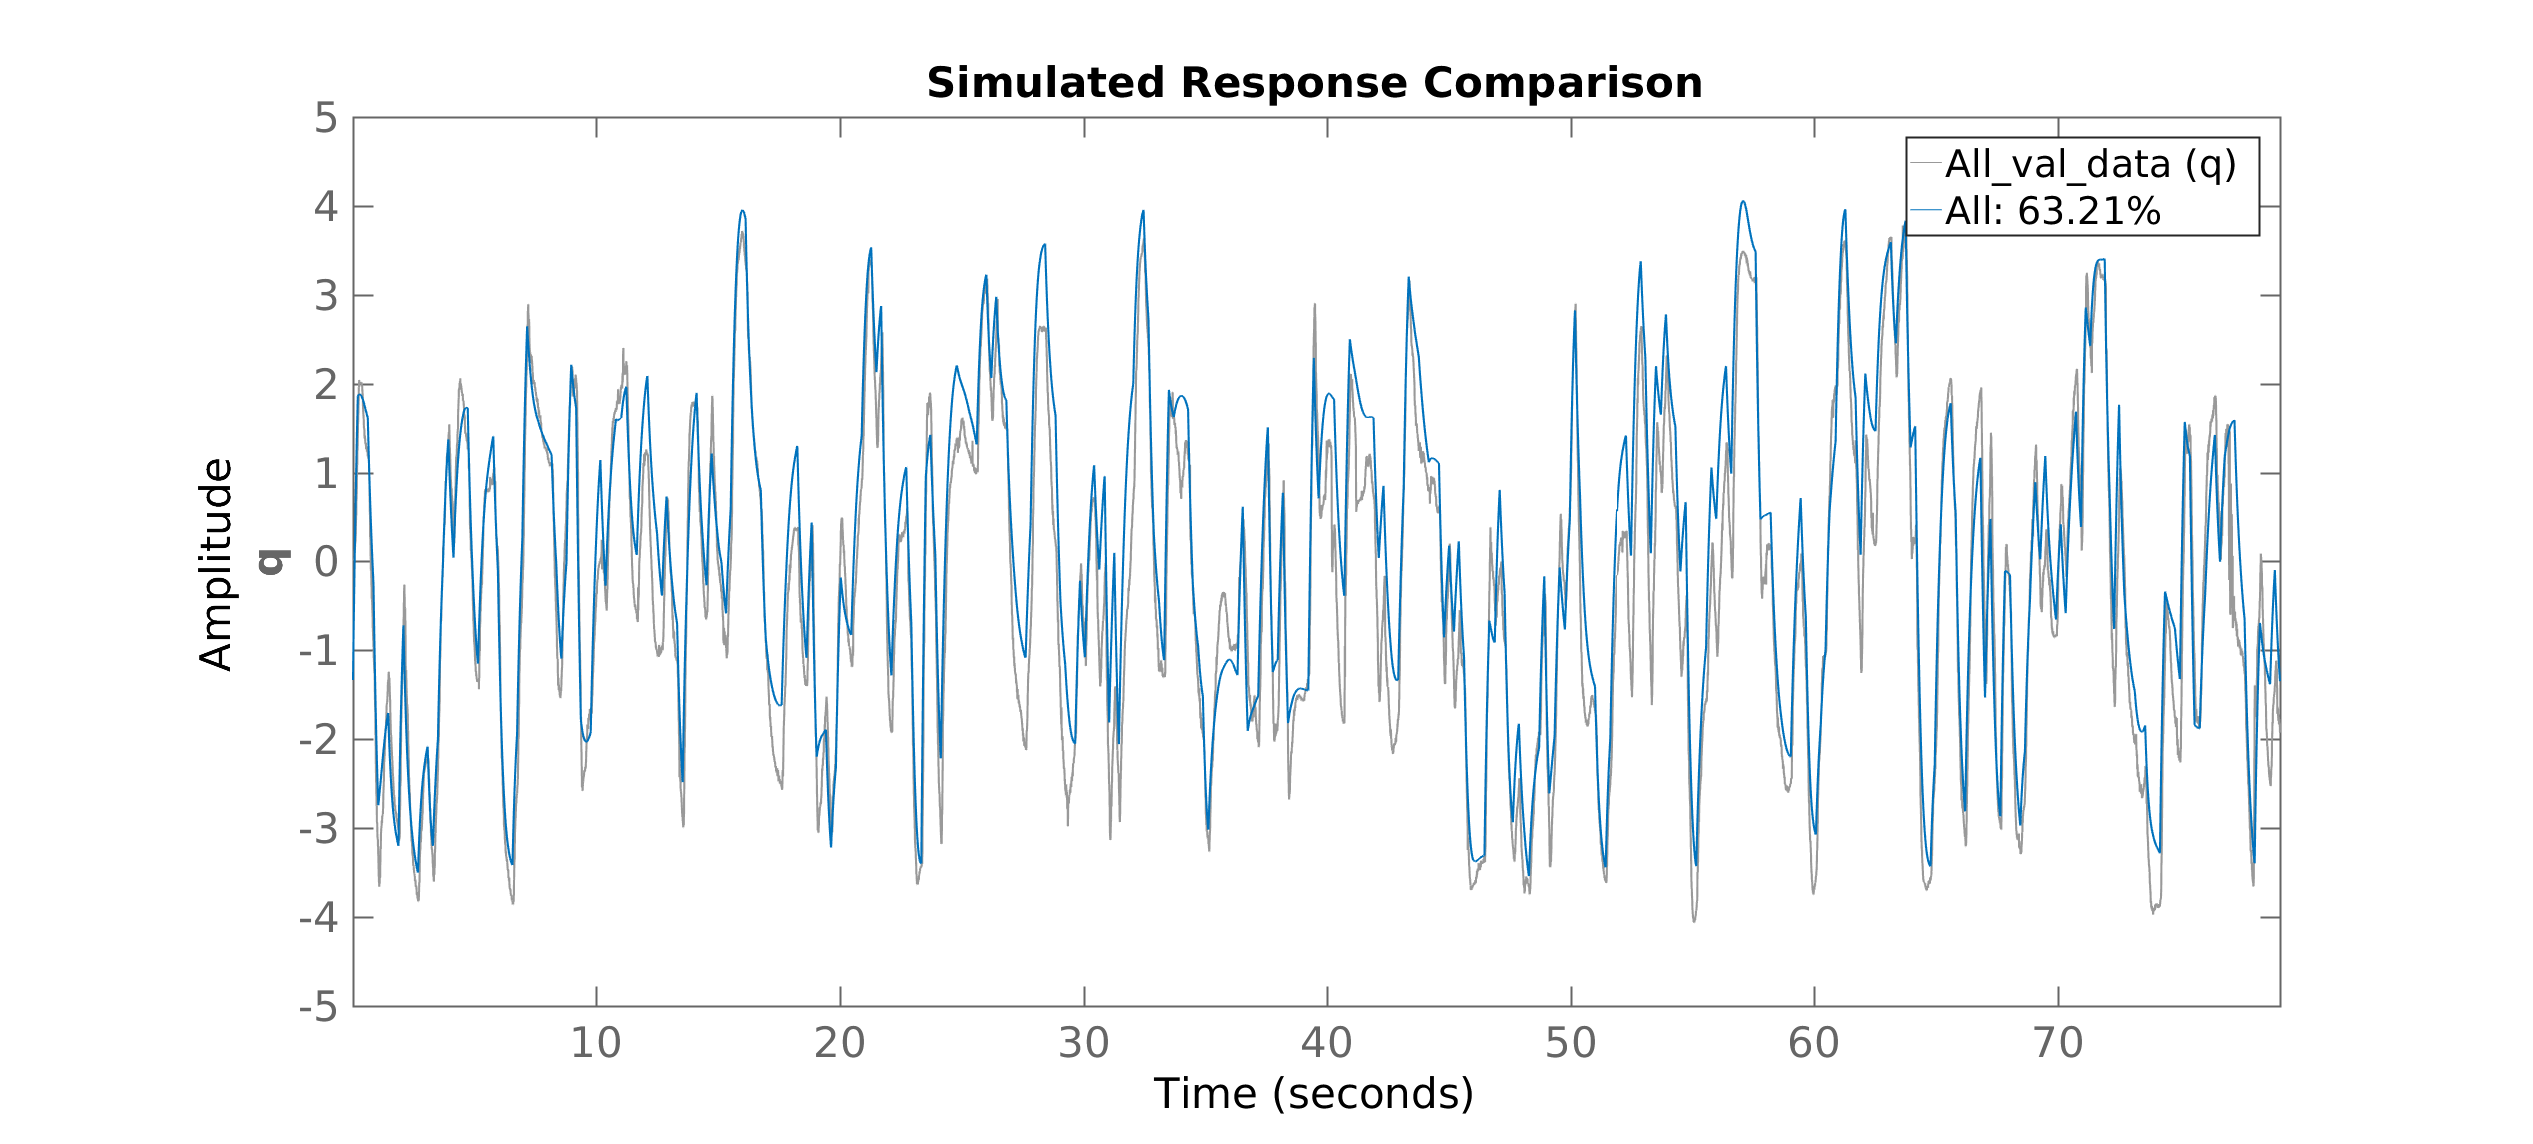
\includegraphics[width=0.4\textwidth]{velocityCompareq}}
  \qquad
  \subfloat[][\label{fig:testStepQ} An step was applied to $\pitchVelocity$ .]{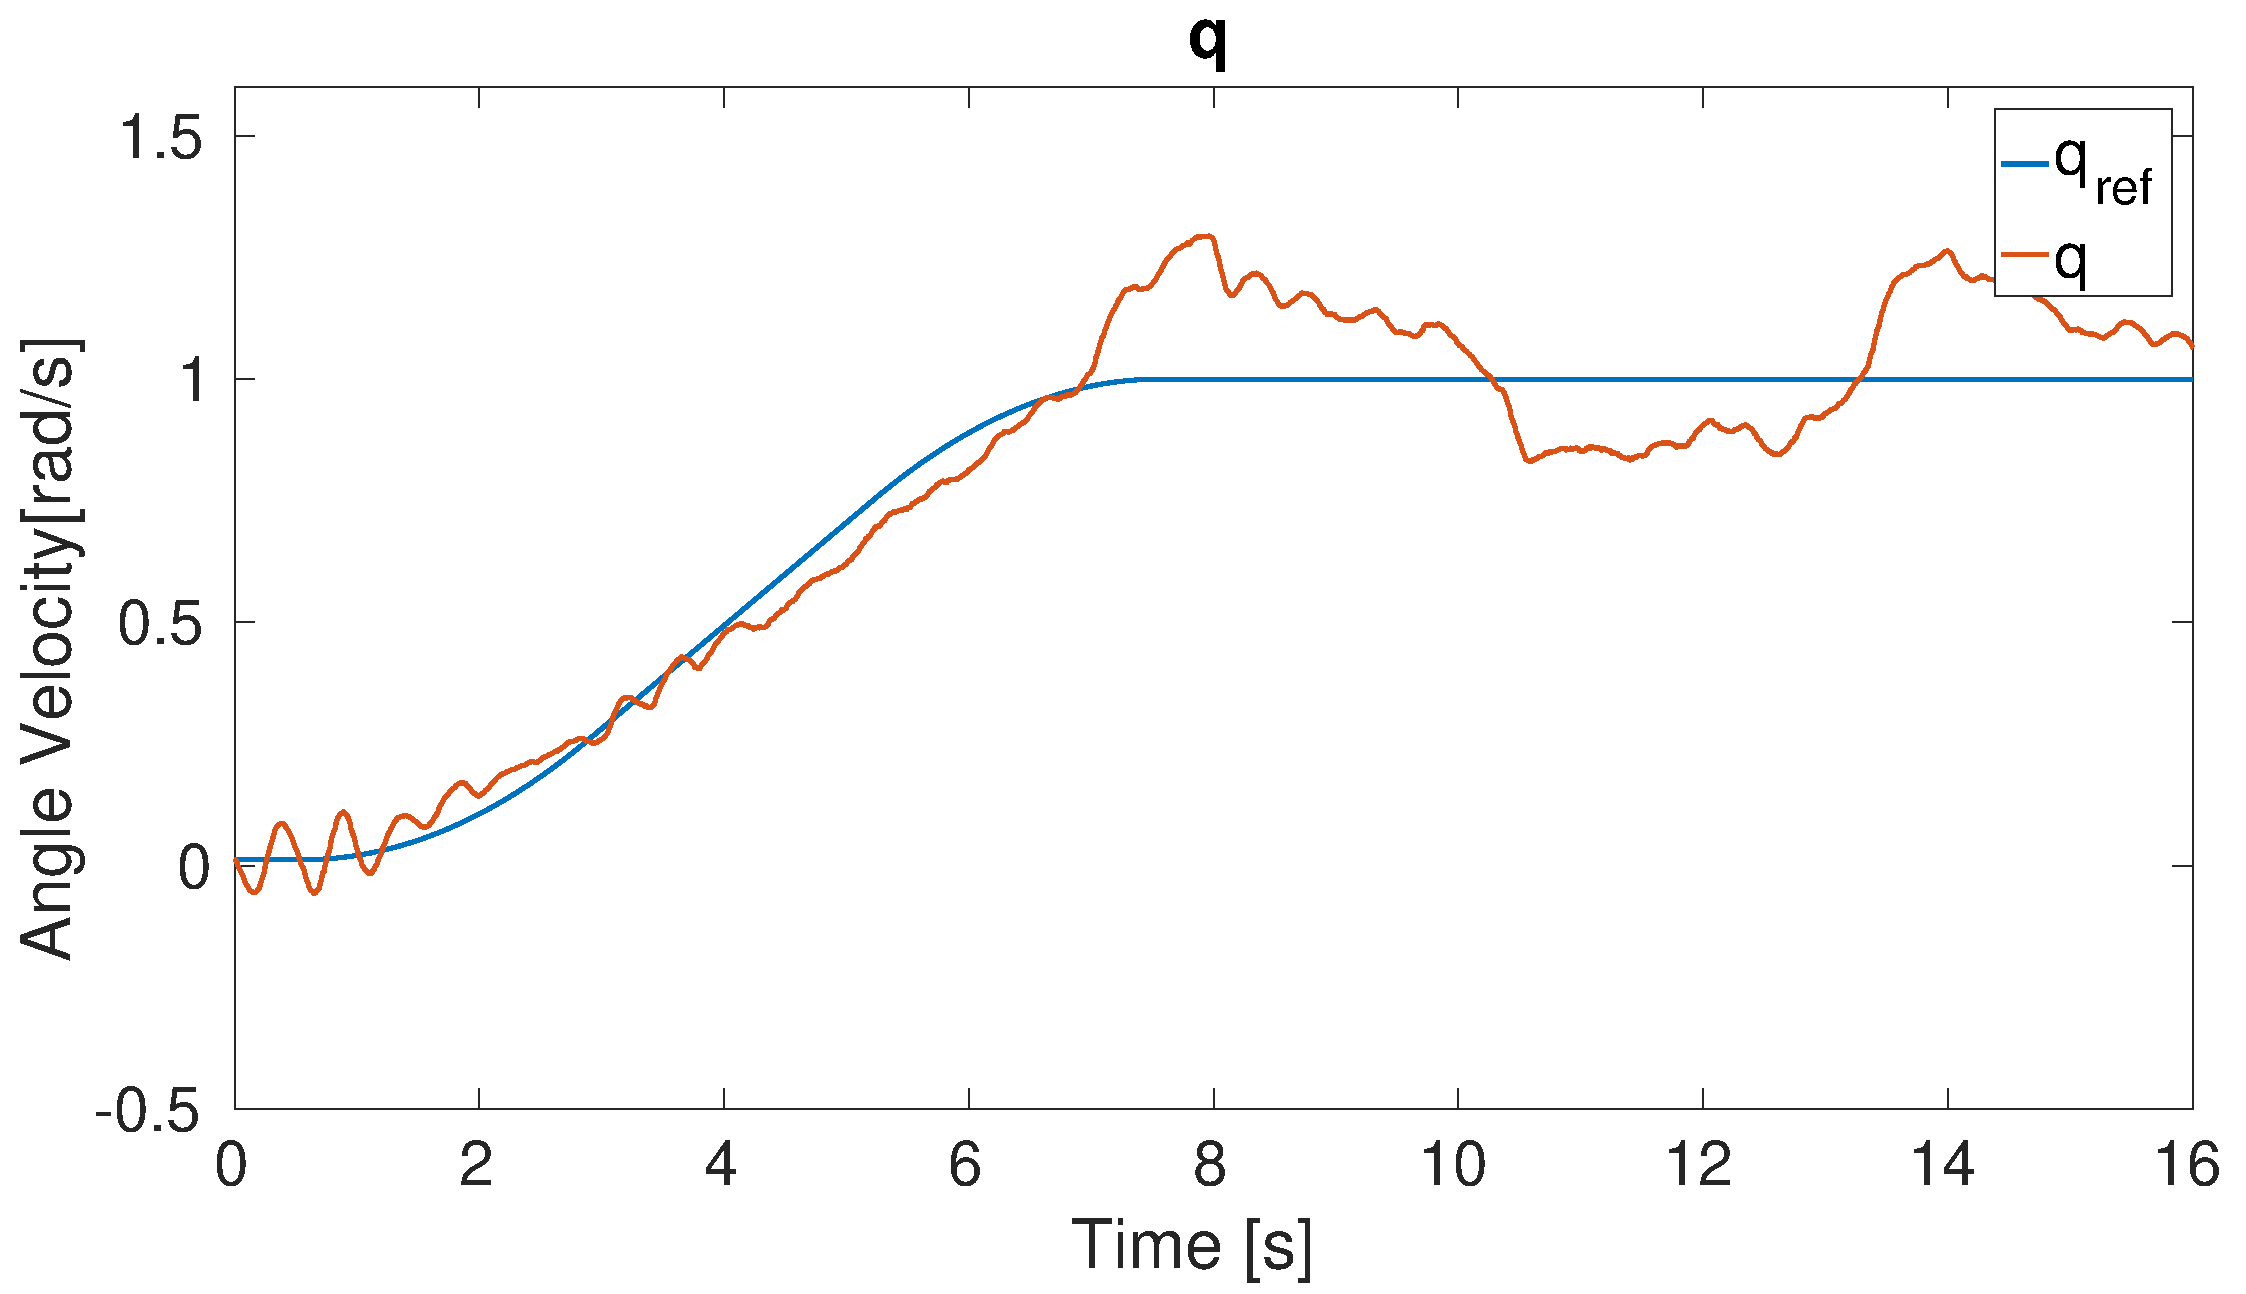
\includegraphics[width=0.4\textwidth]{testStepQs3e10a1}}
  \qquad
  \subfloat[][\label{fig:simStepQ} An step was applied to the simulated \abbrROV in $\pitchVelocity$.]{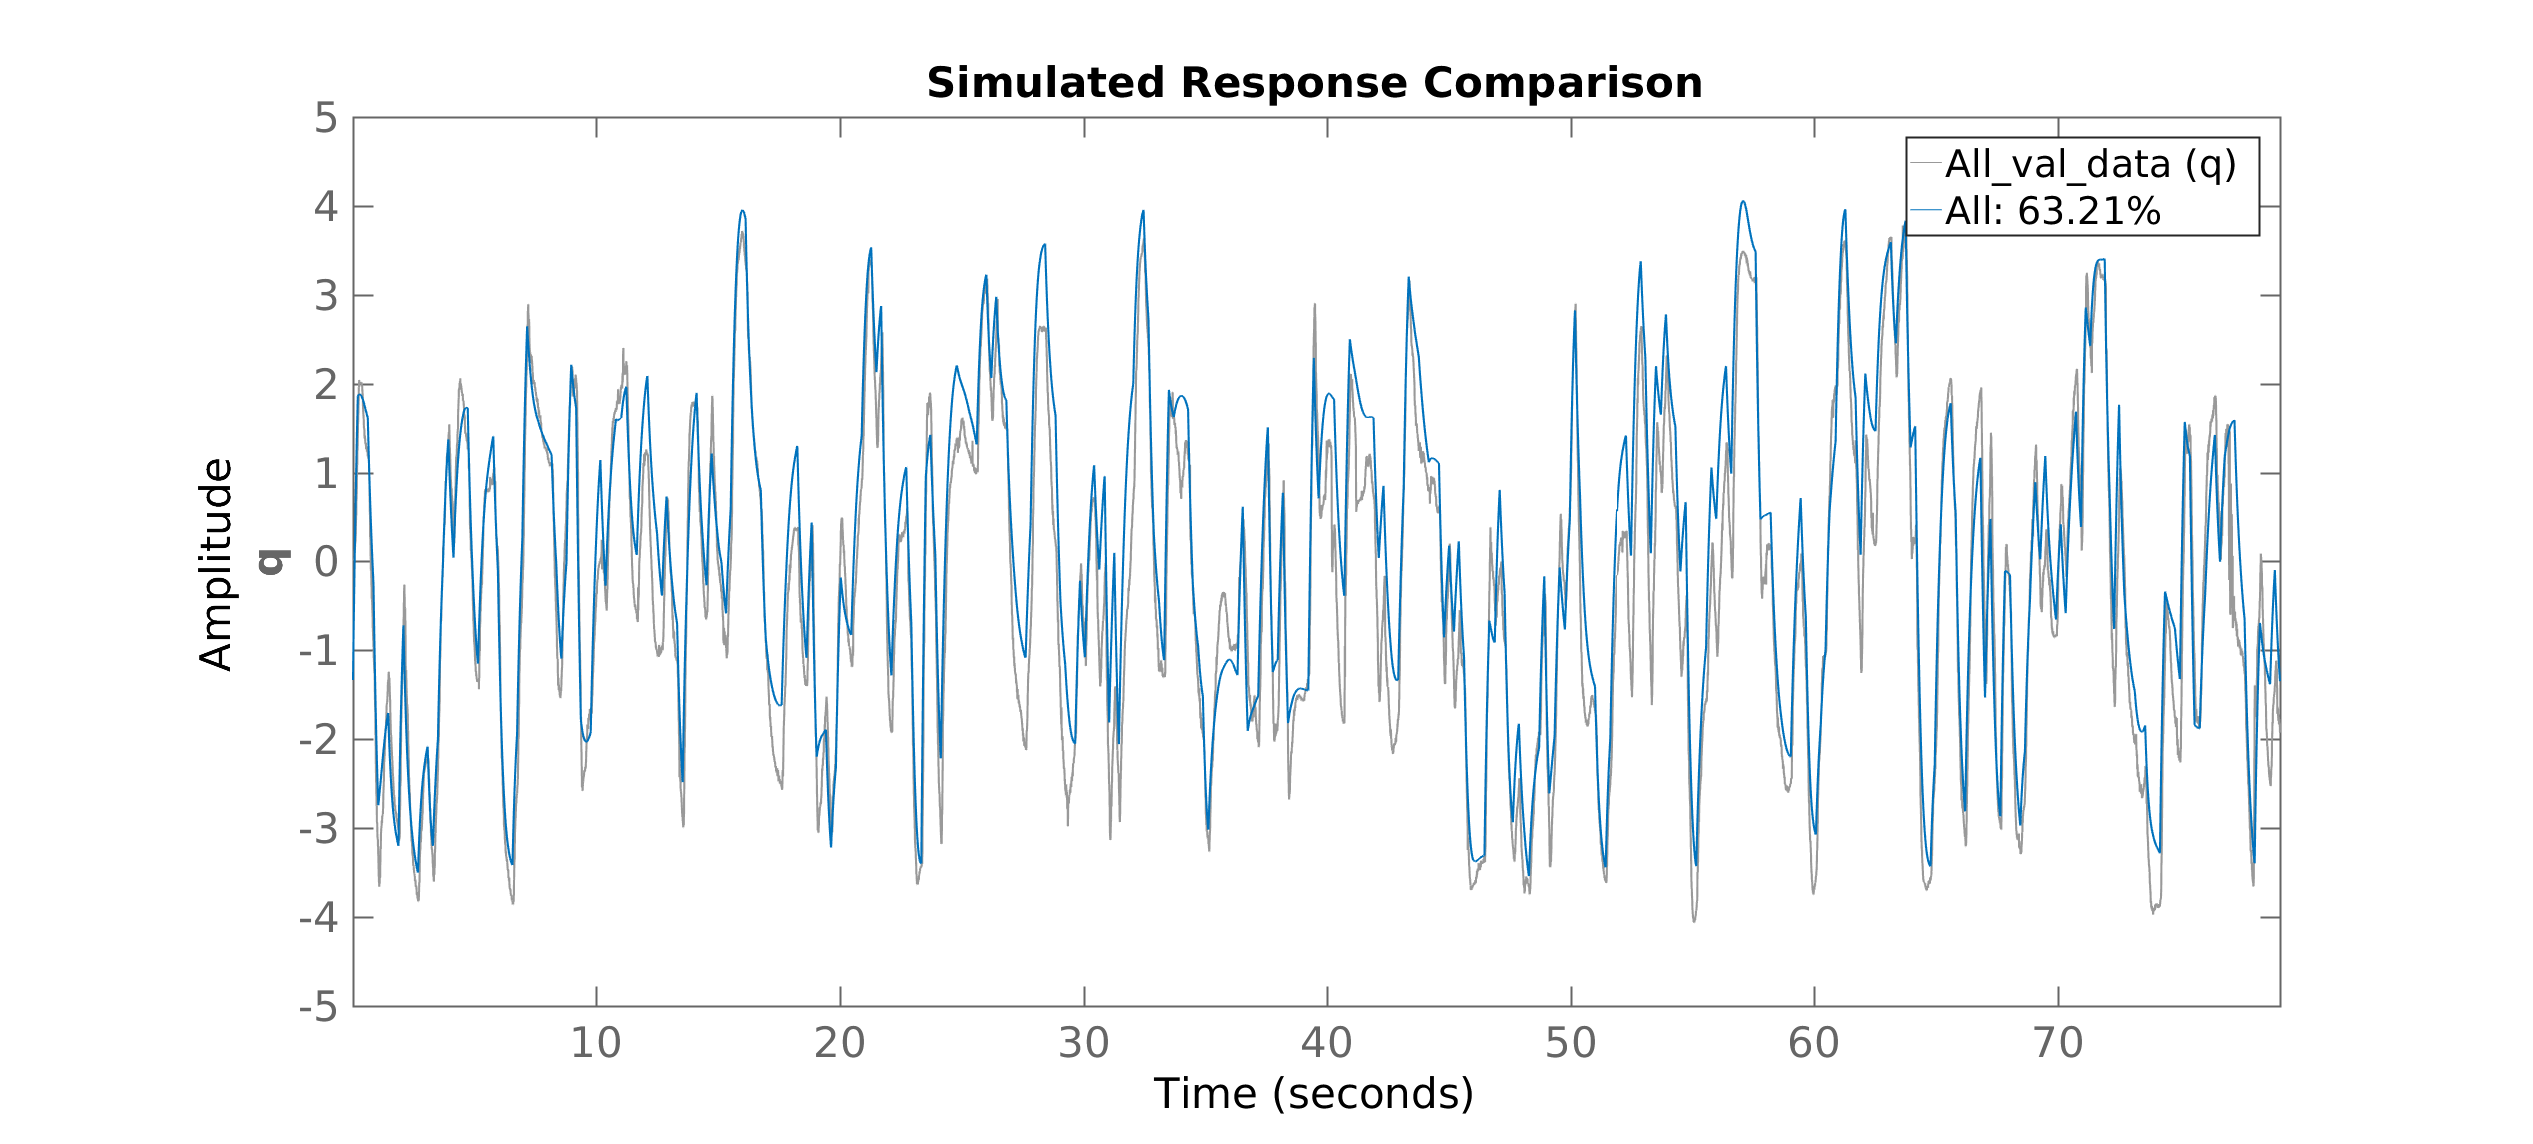
\includegraphics[width=0.4\textwidth]{velocityCompareq}}
  \qquad
  \subfloat[][\label{fig:testStepR} An step was applied to $\yawVelocity$ .]{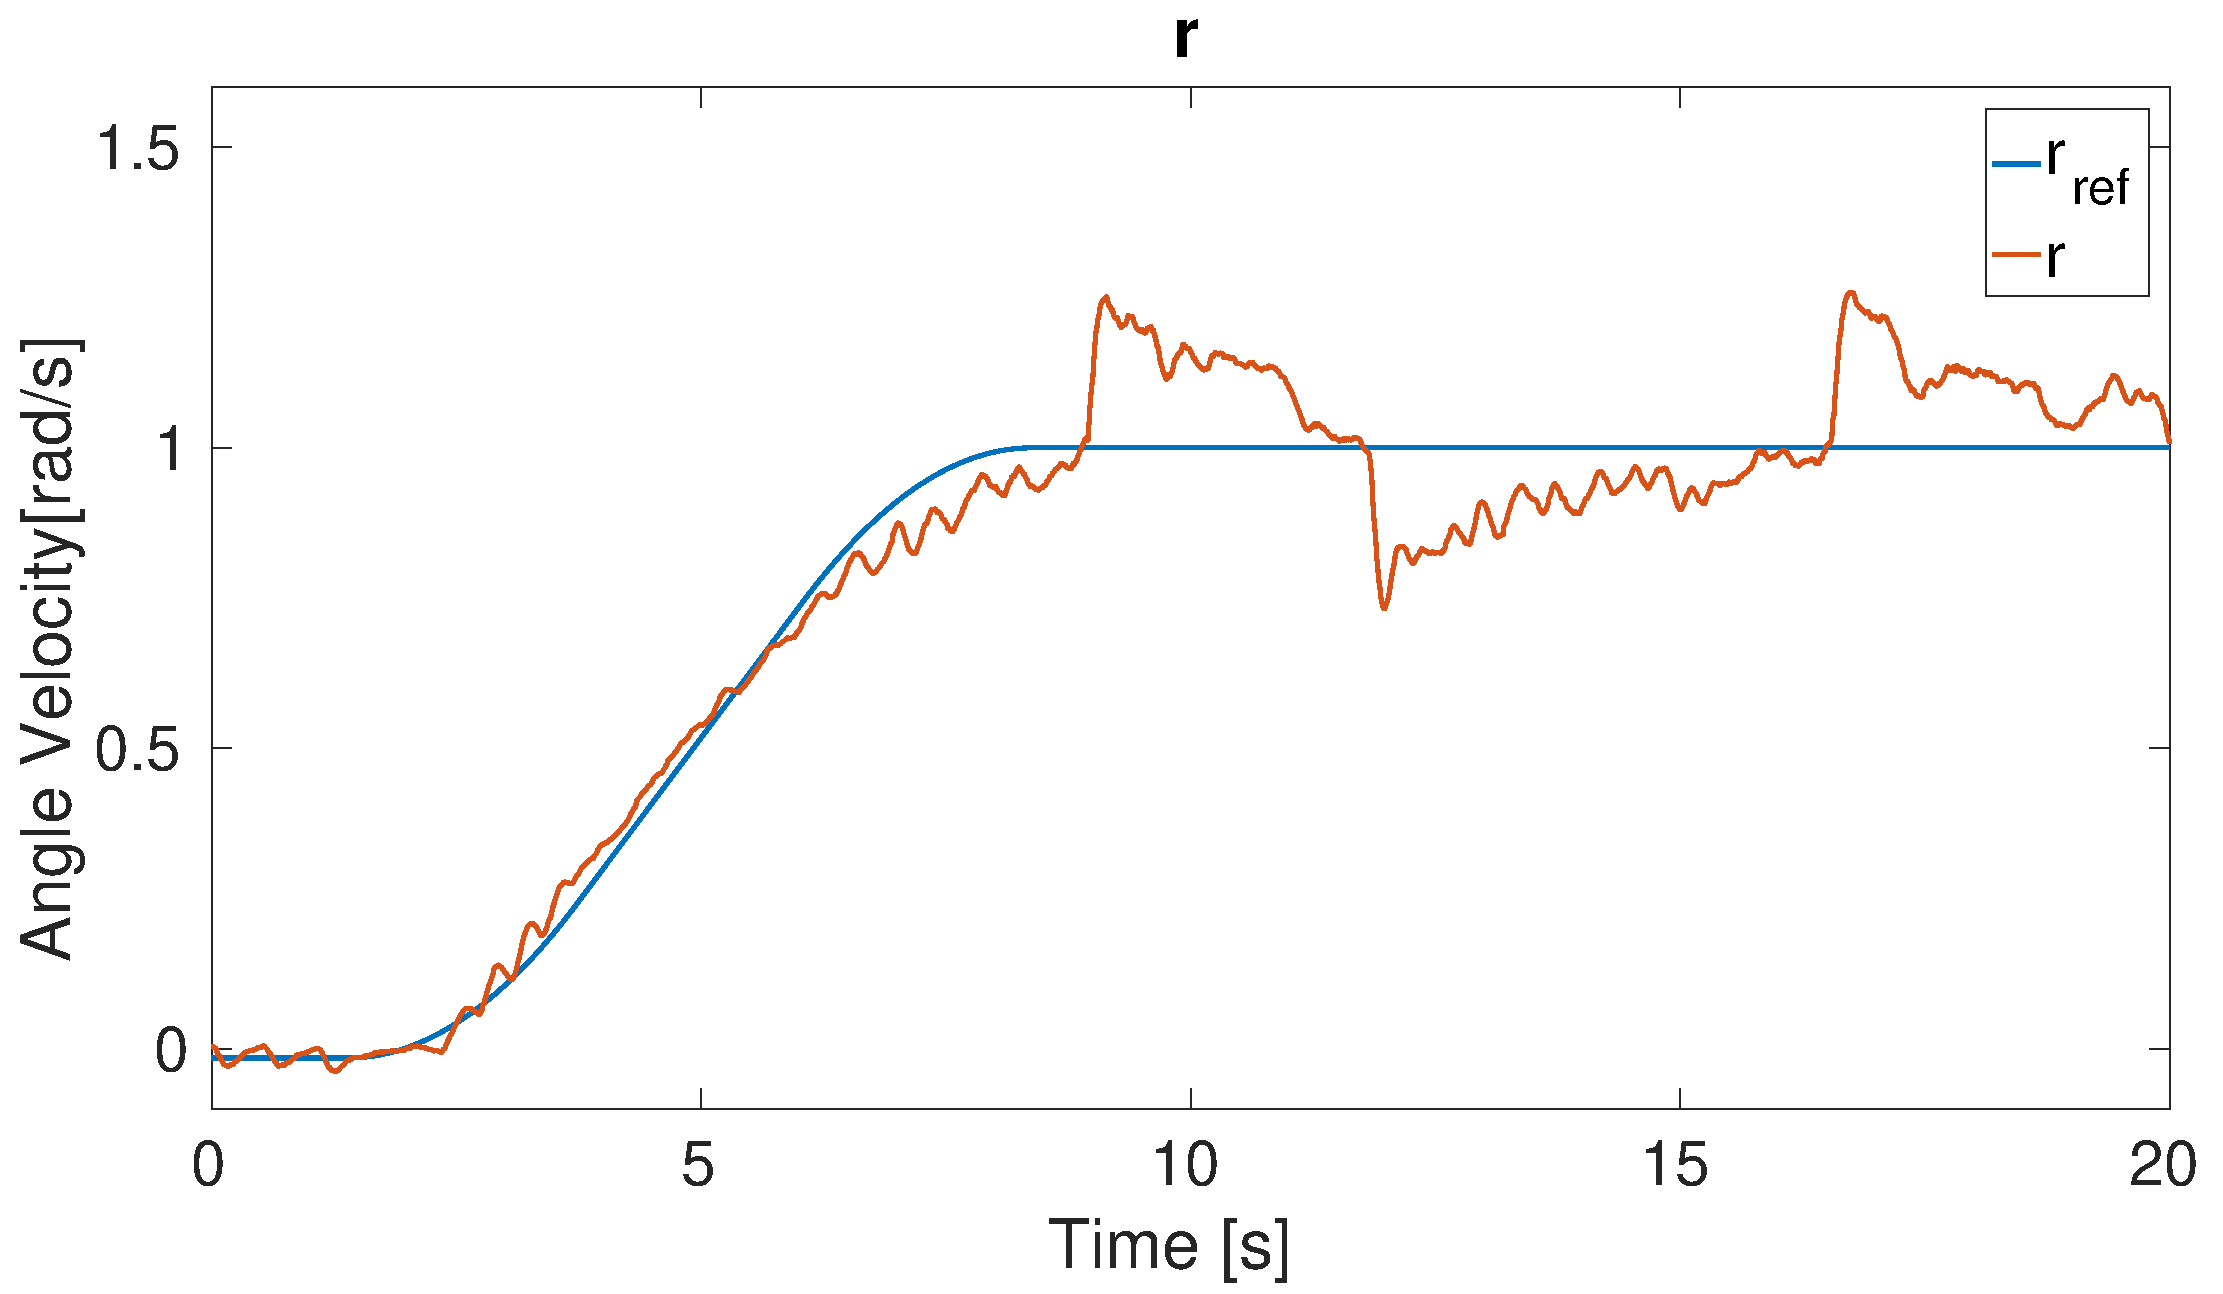
\includegraphics[width=0.4\textwidth]{testStepRs3e10a1}}
  \qquad
  \subfloat[][\label{fig:simStepR} An step was applied to the simulated \abbrROV in $\yawVelocity$.]{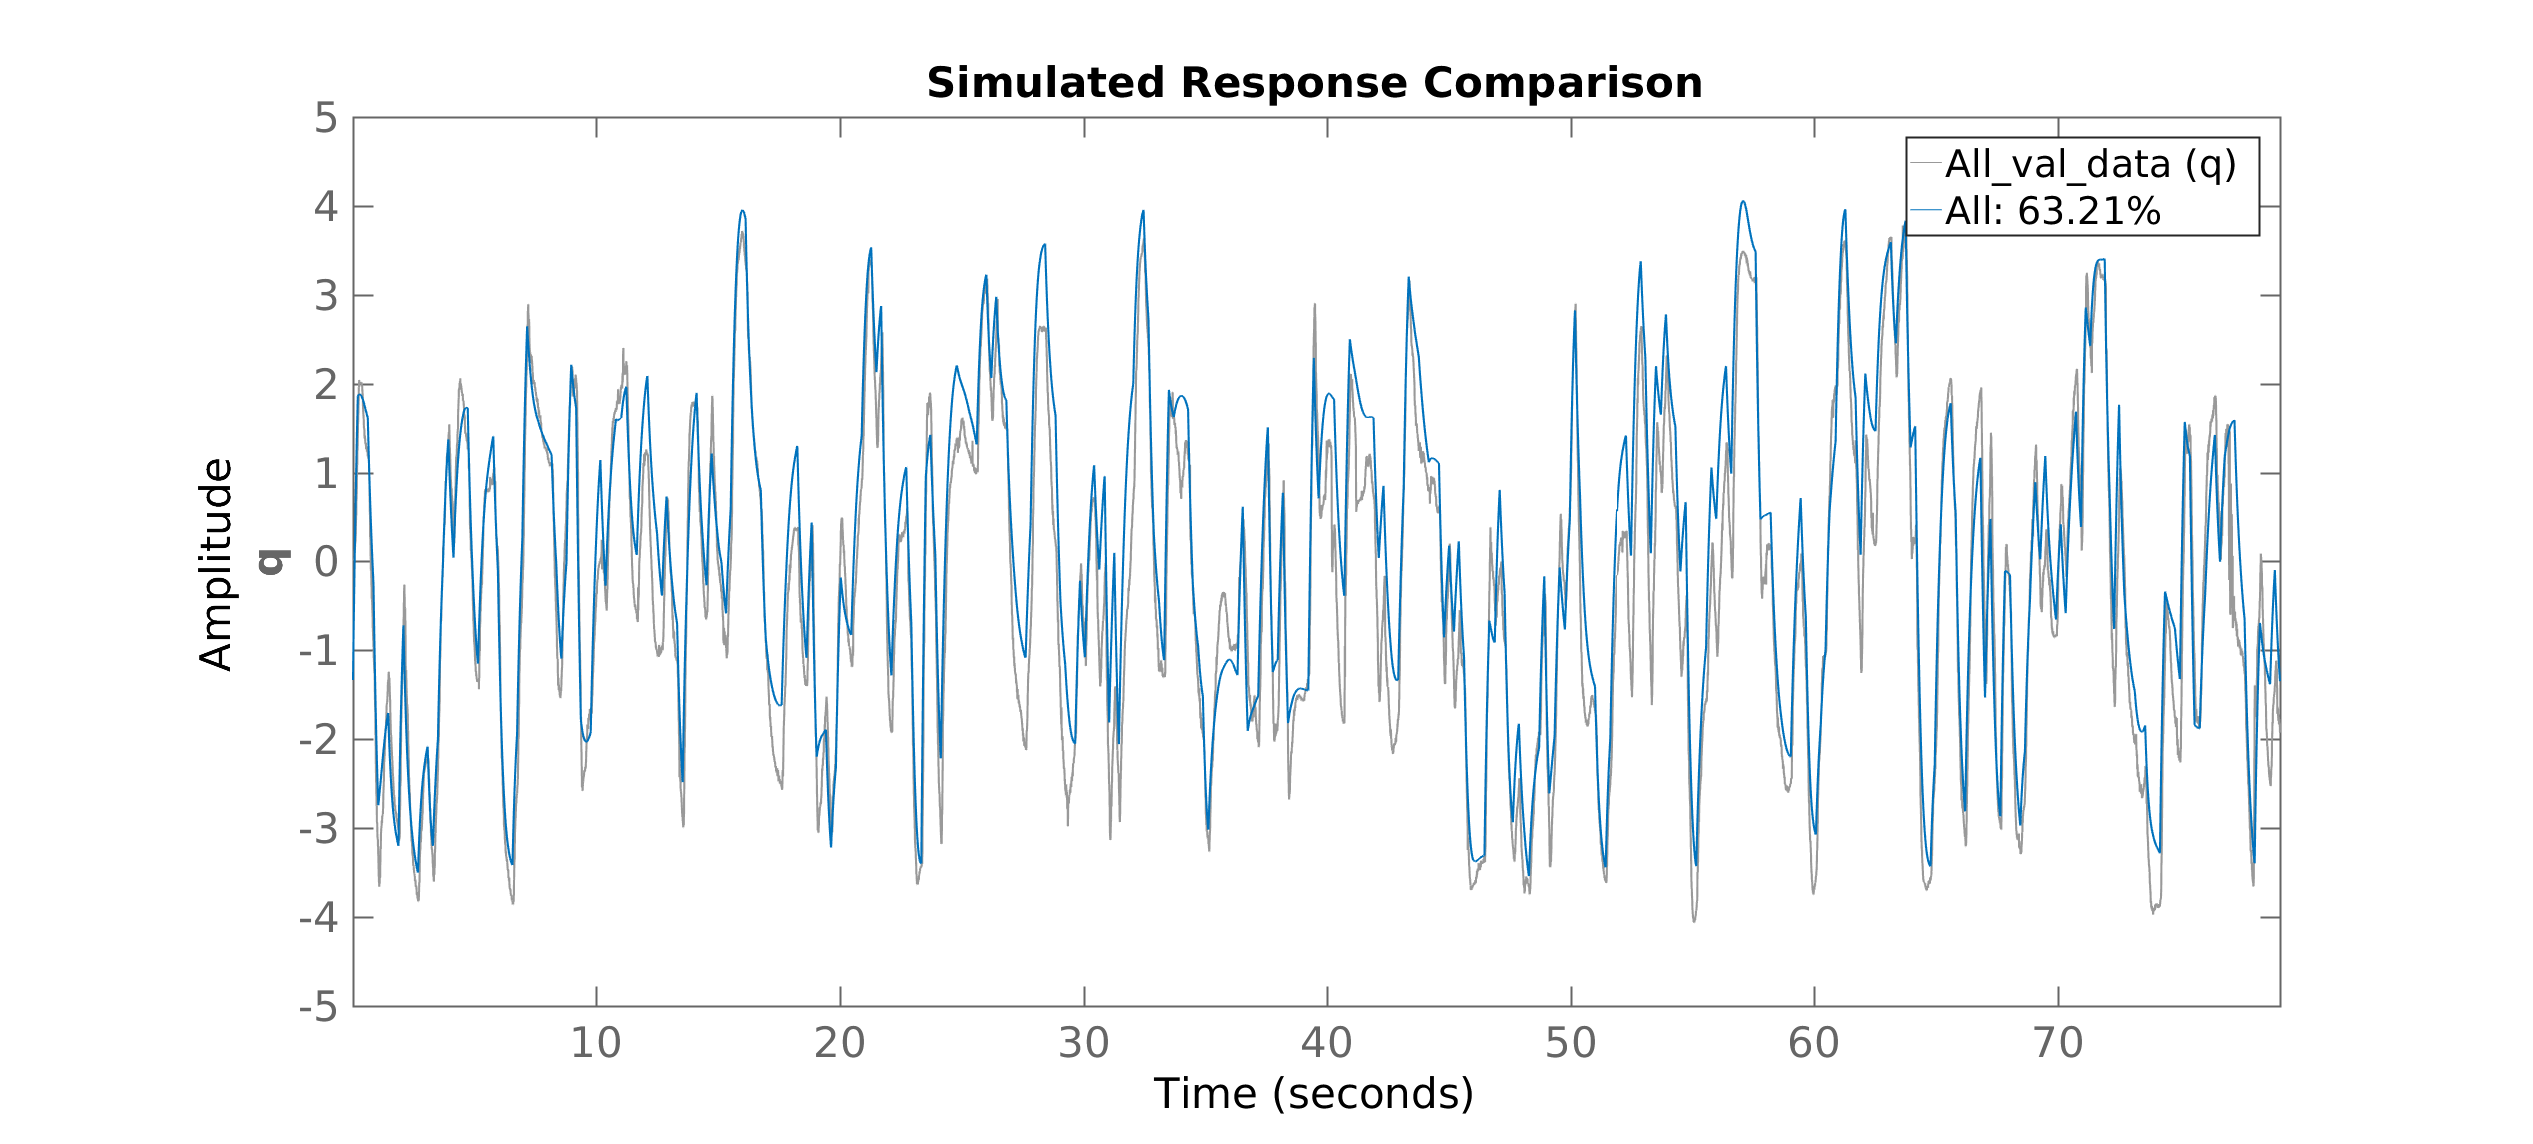
\includegraphics[width=0.4\textwidth]{velocityCompareq}}
   \caption{\label{fig:StepRate}%
    Comparison between simulation and a real test of a smooth step reference in.}
\end{figure}

\begin{figure}
\centering
  \subfloat[][\label{fig:testStepAllPRate} An step was applied to all \abbrDOF.]{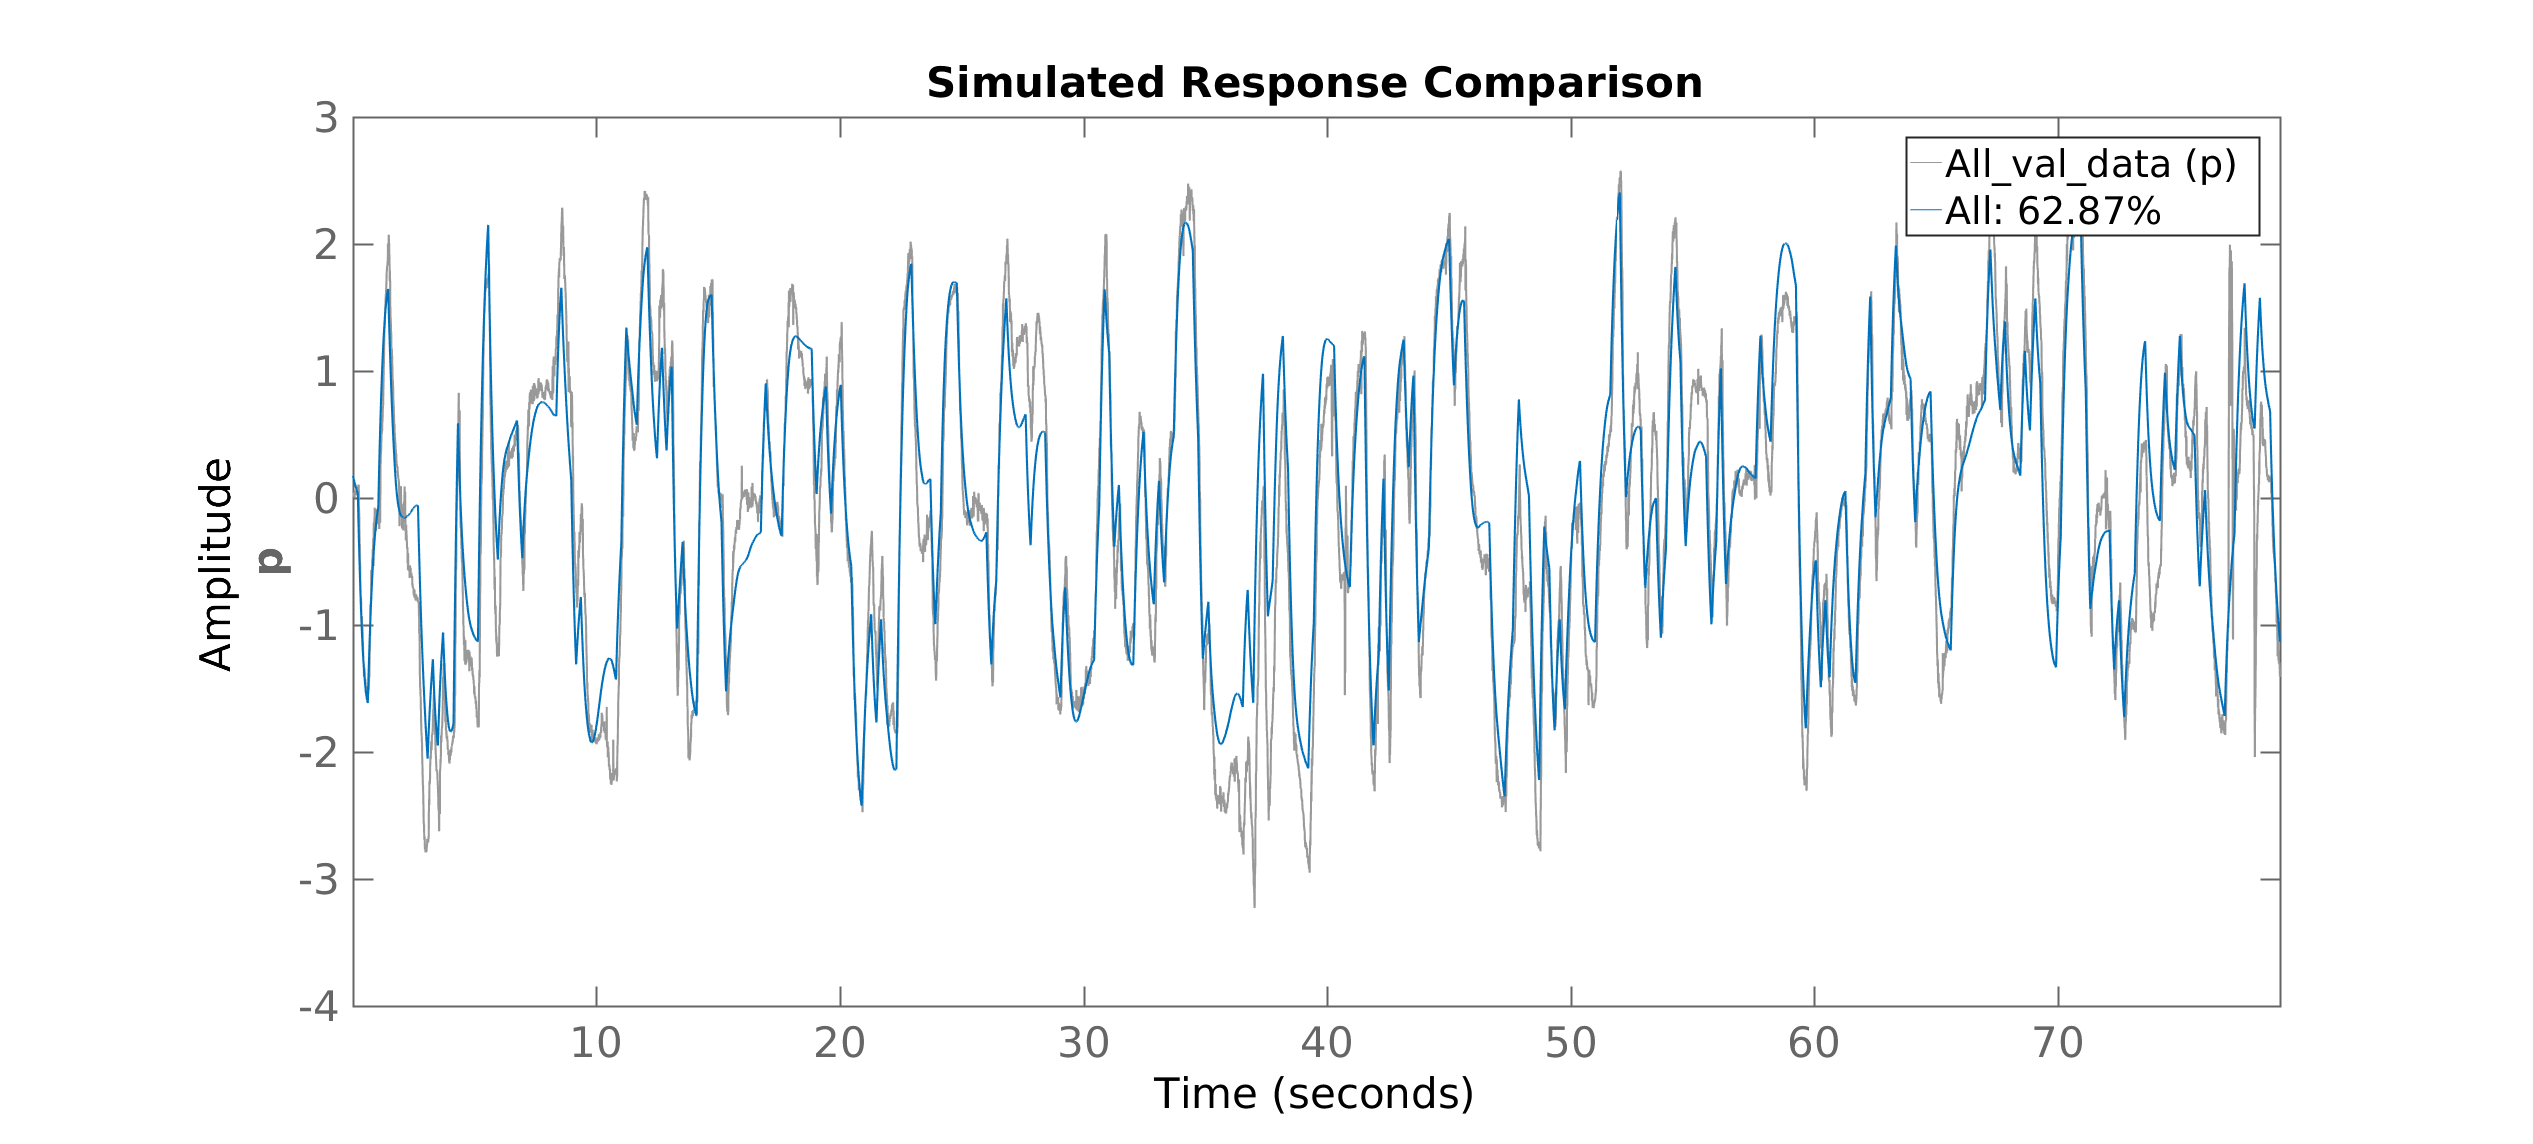
\includegraphics[width=0.4\textwidth]{velocityComparep}}
  \qquad
  \subfloat[][\label{fig:simStepAllPRate} An step was applied to the simulated \abbrROV in all \abbrDOF.]{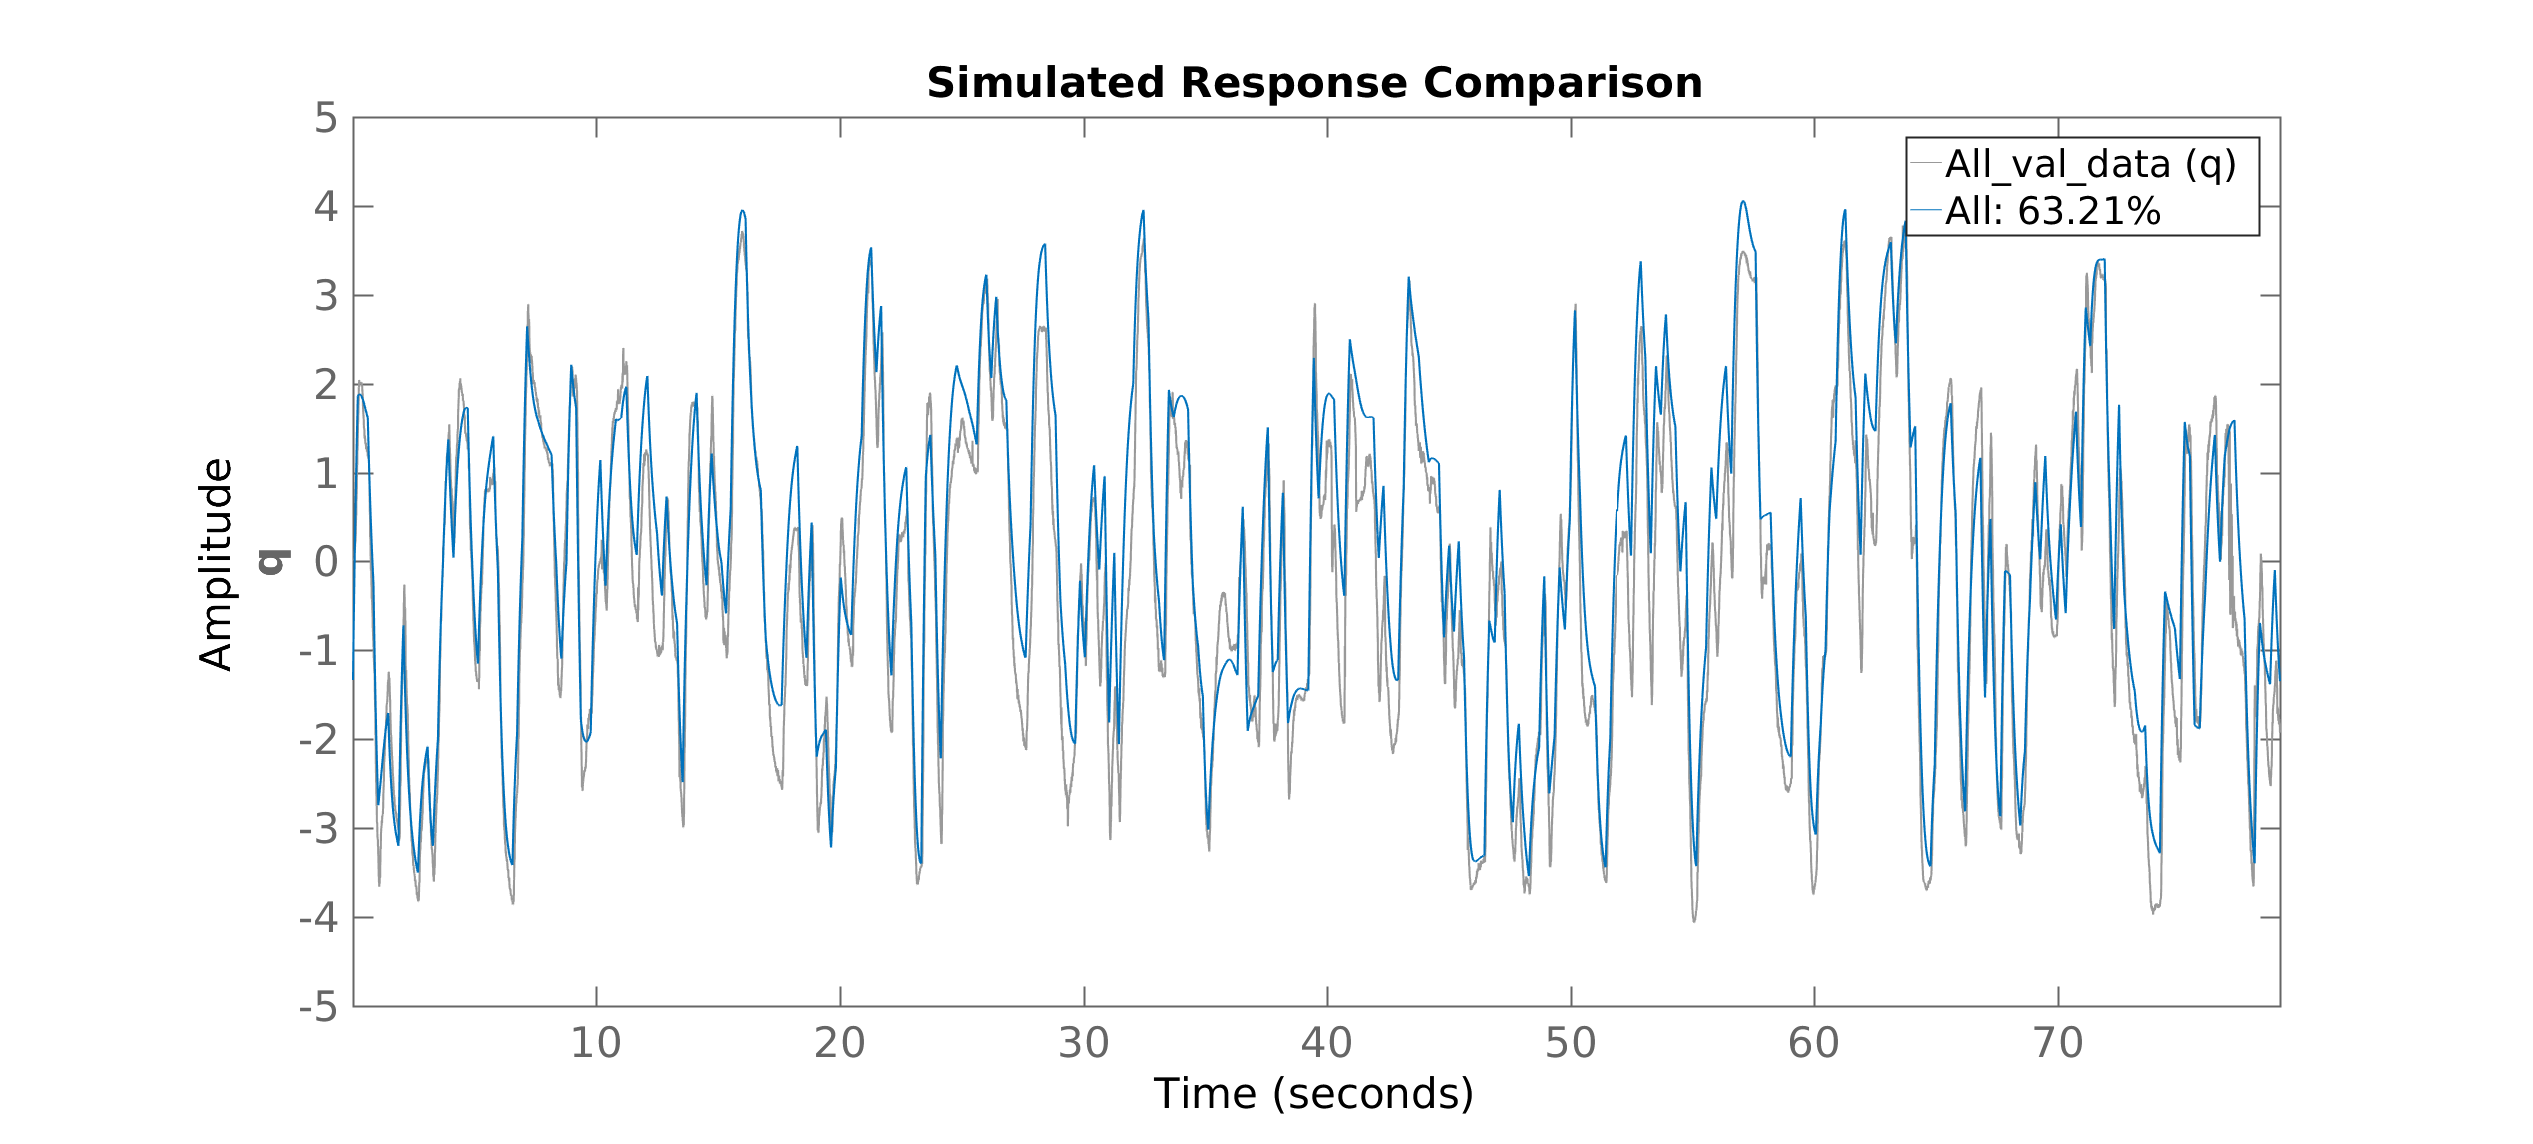
\includegraphics[width=0.4\textwidth]{velocityCompareq}}
  \qquad
  \subfloat[][\label{fig:simStepAllQRate} An step was applied to the simulated \abbrROV in all \abbrDOF.]{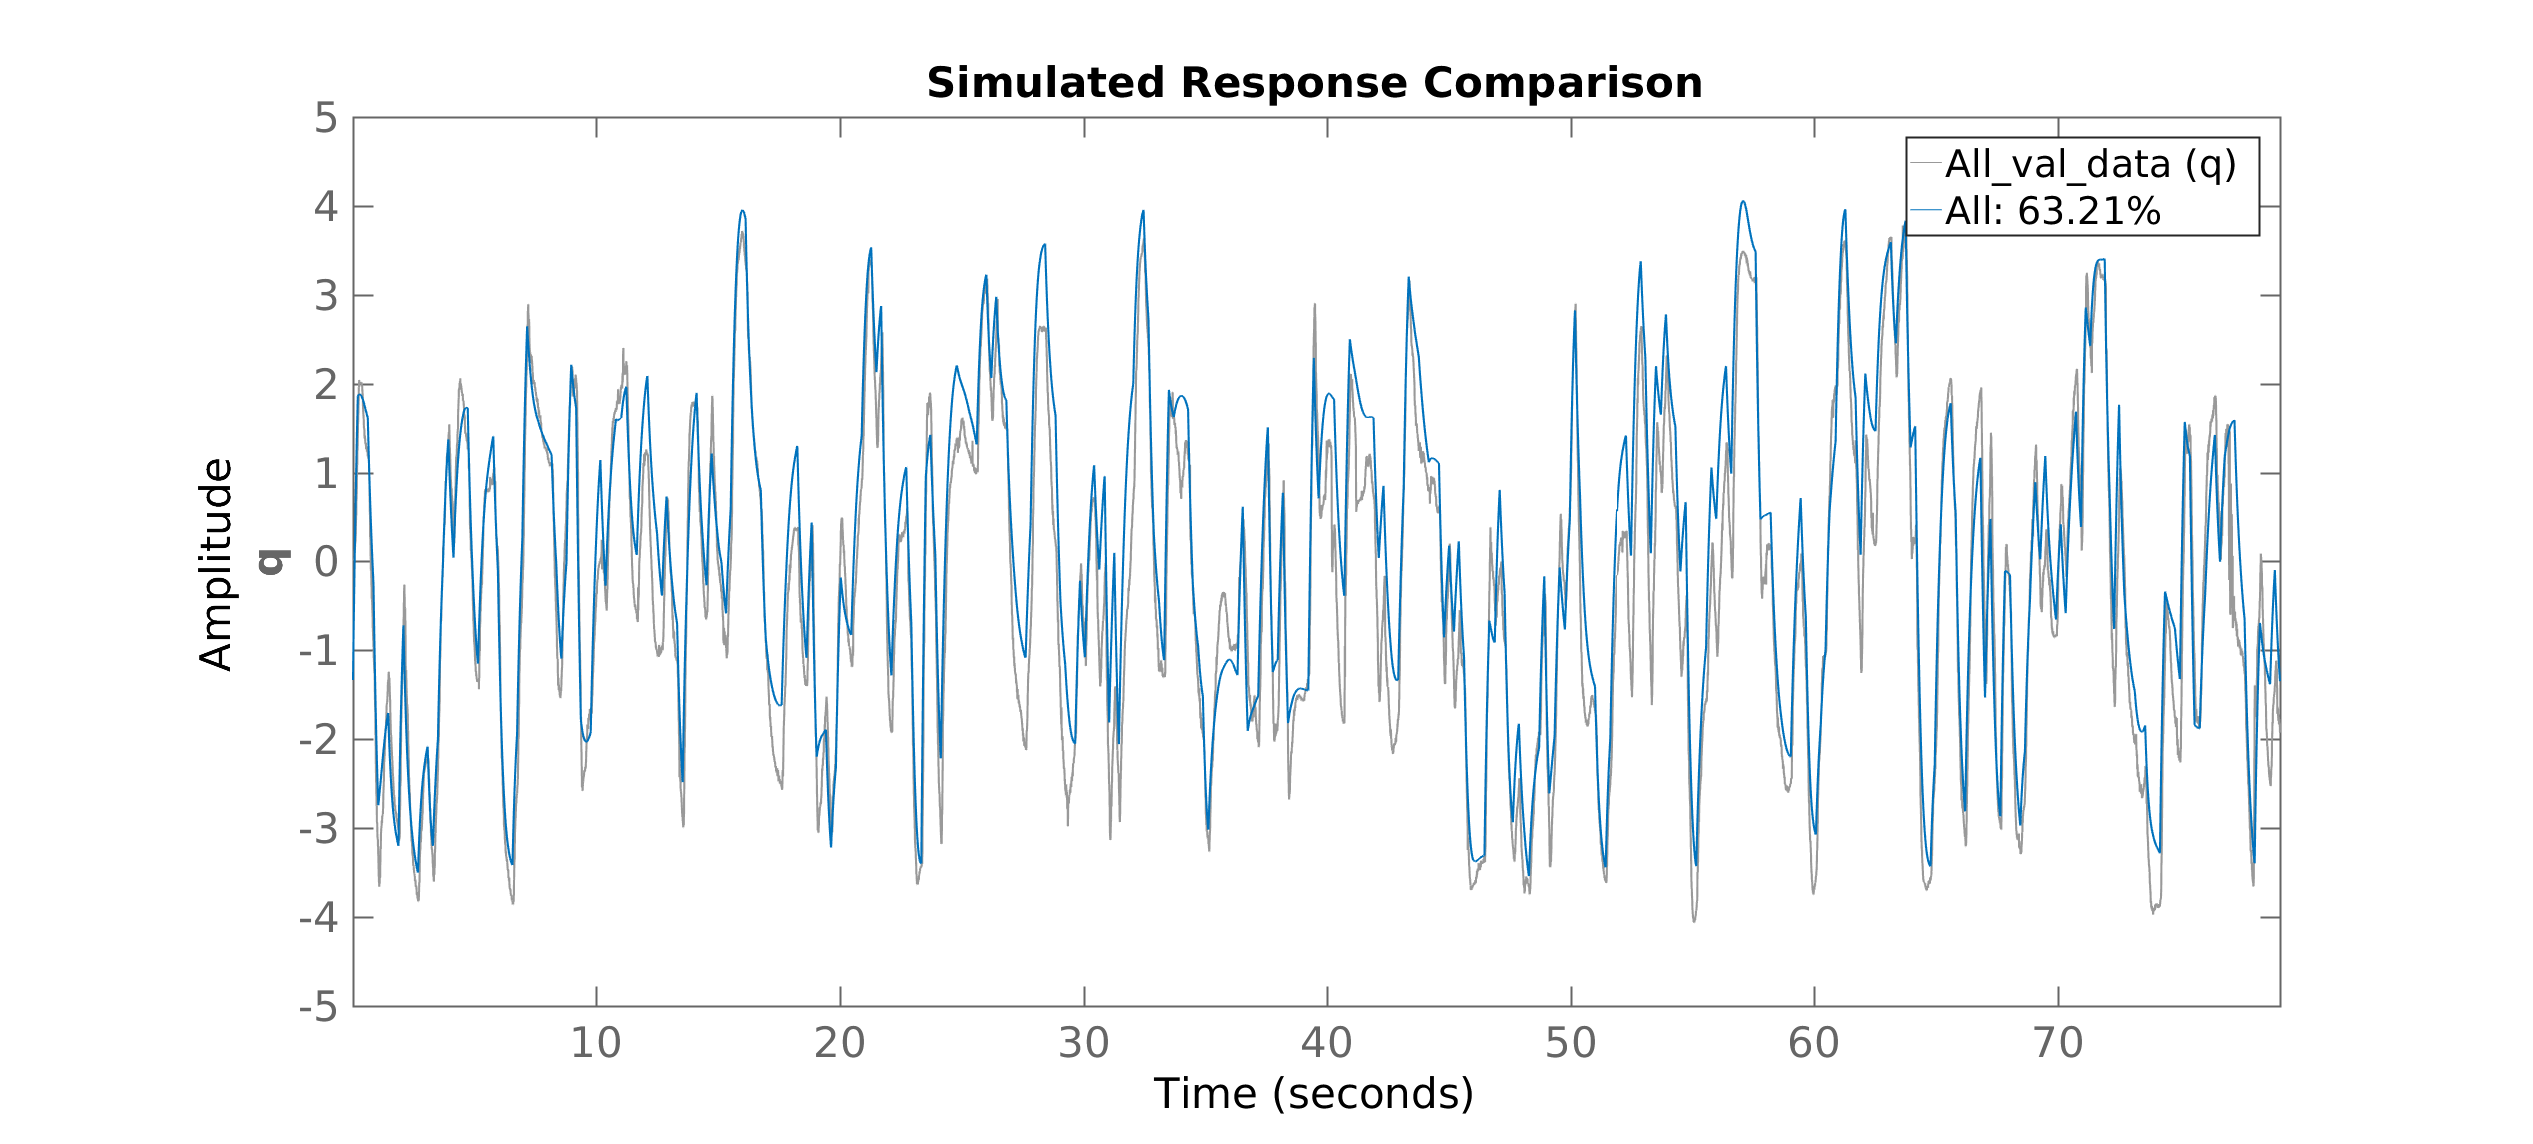
\includegraphics[width=0.4\textwidth]{velocityCompareq}}
  \qquad
  \subfloat[][\label{fig:simStepAllQRate} An step was applied to the simulated \abbrROV in all \abbrDOF.]{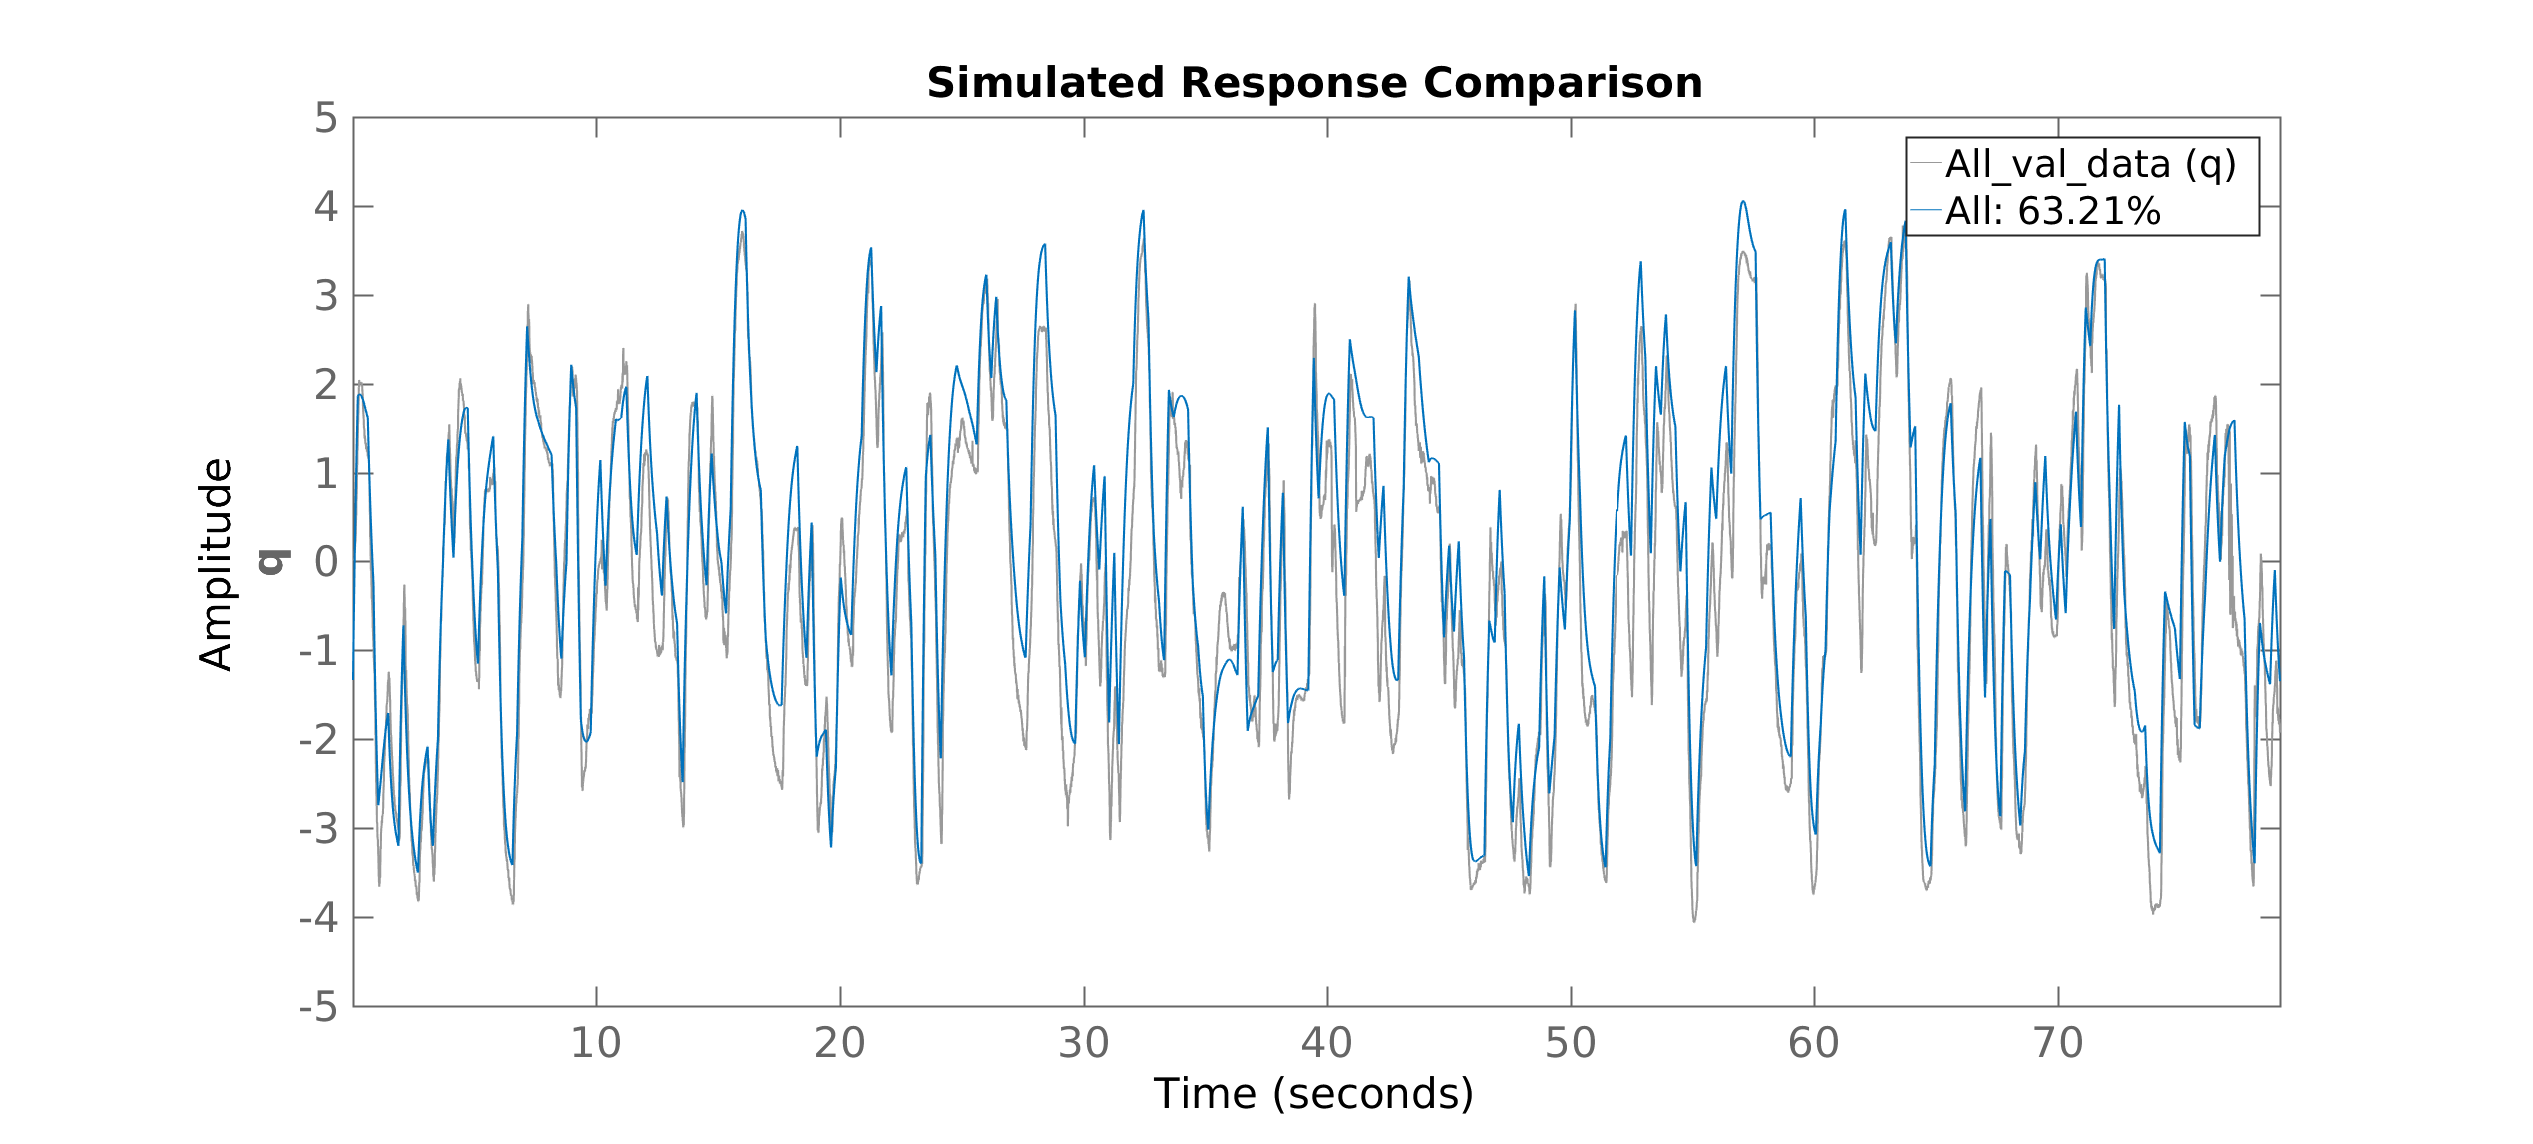
\includegraphics[width=0.4\textwidth]{velocityCompareq}}
  \qquad
  \subfloat[][\label{fig:simStepAllRRate} An step was applied to the simulated \abbrROV in all \abbrDOF.]{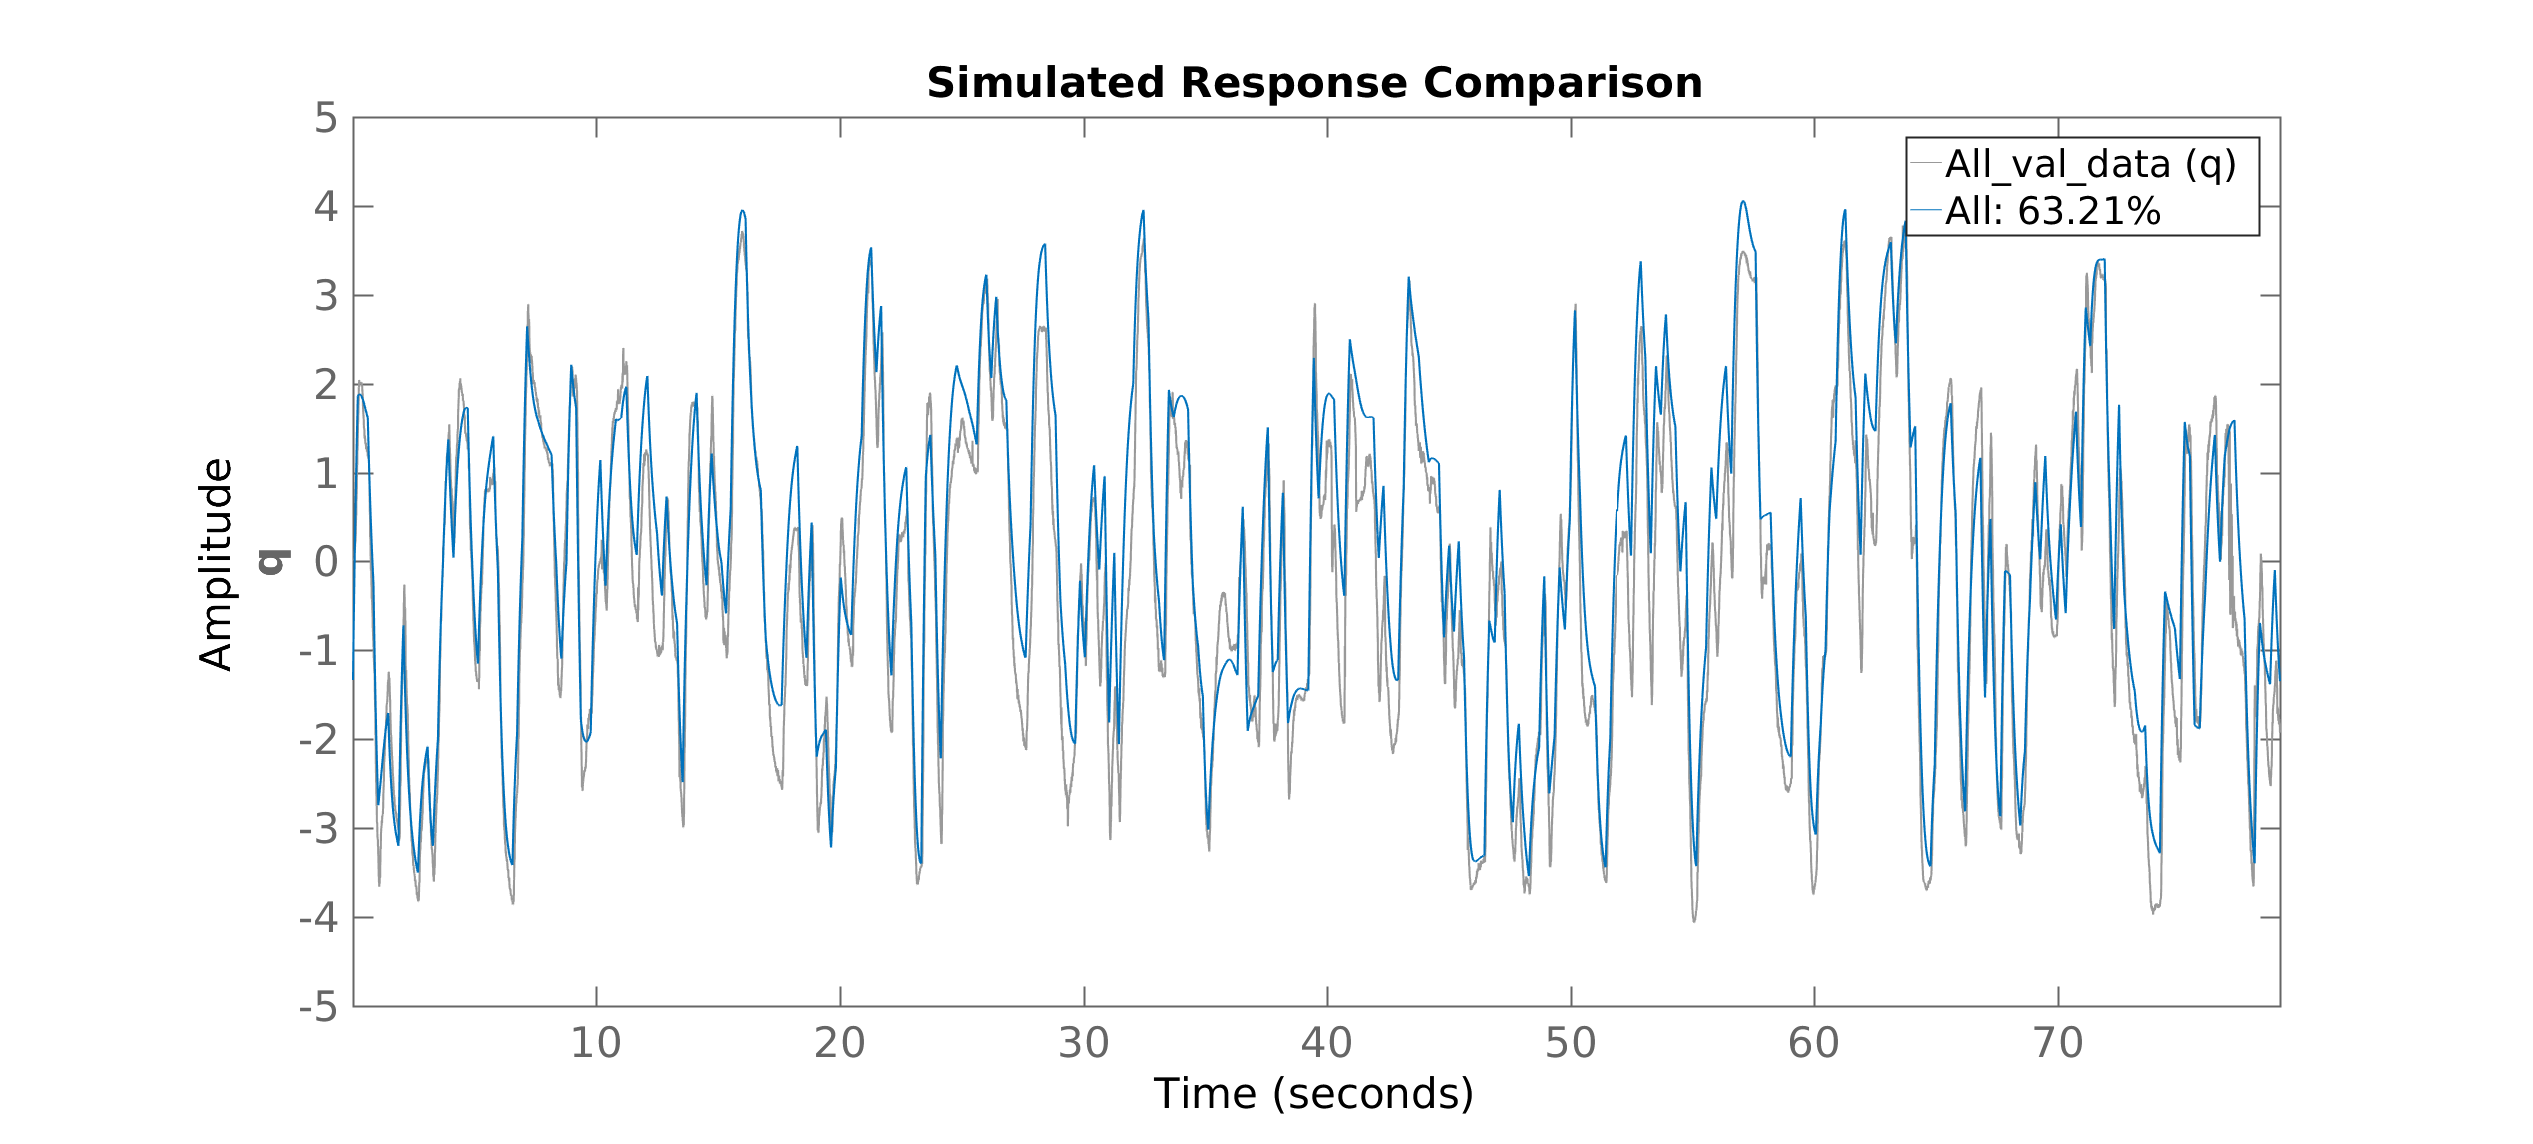
\includegraphics[width=0.4\textwidth]{velocityCompareq}}
  \qquad
  \subfloat[][\label{fig:simStepAllRRate} An step was applied to the simulated \abbrROV in all \abbrDOF.]{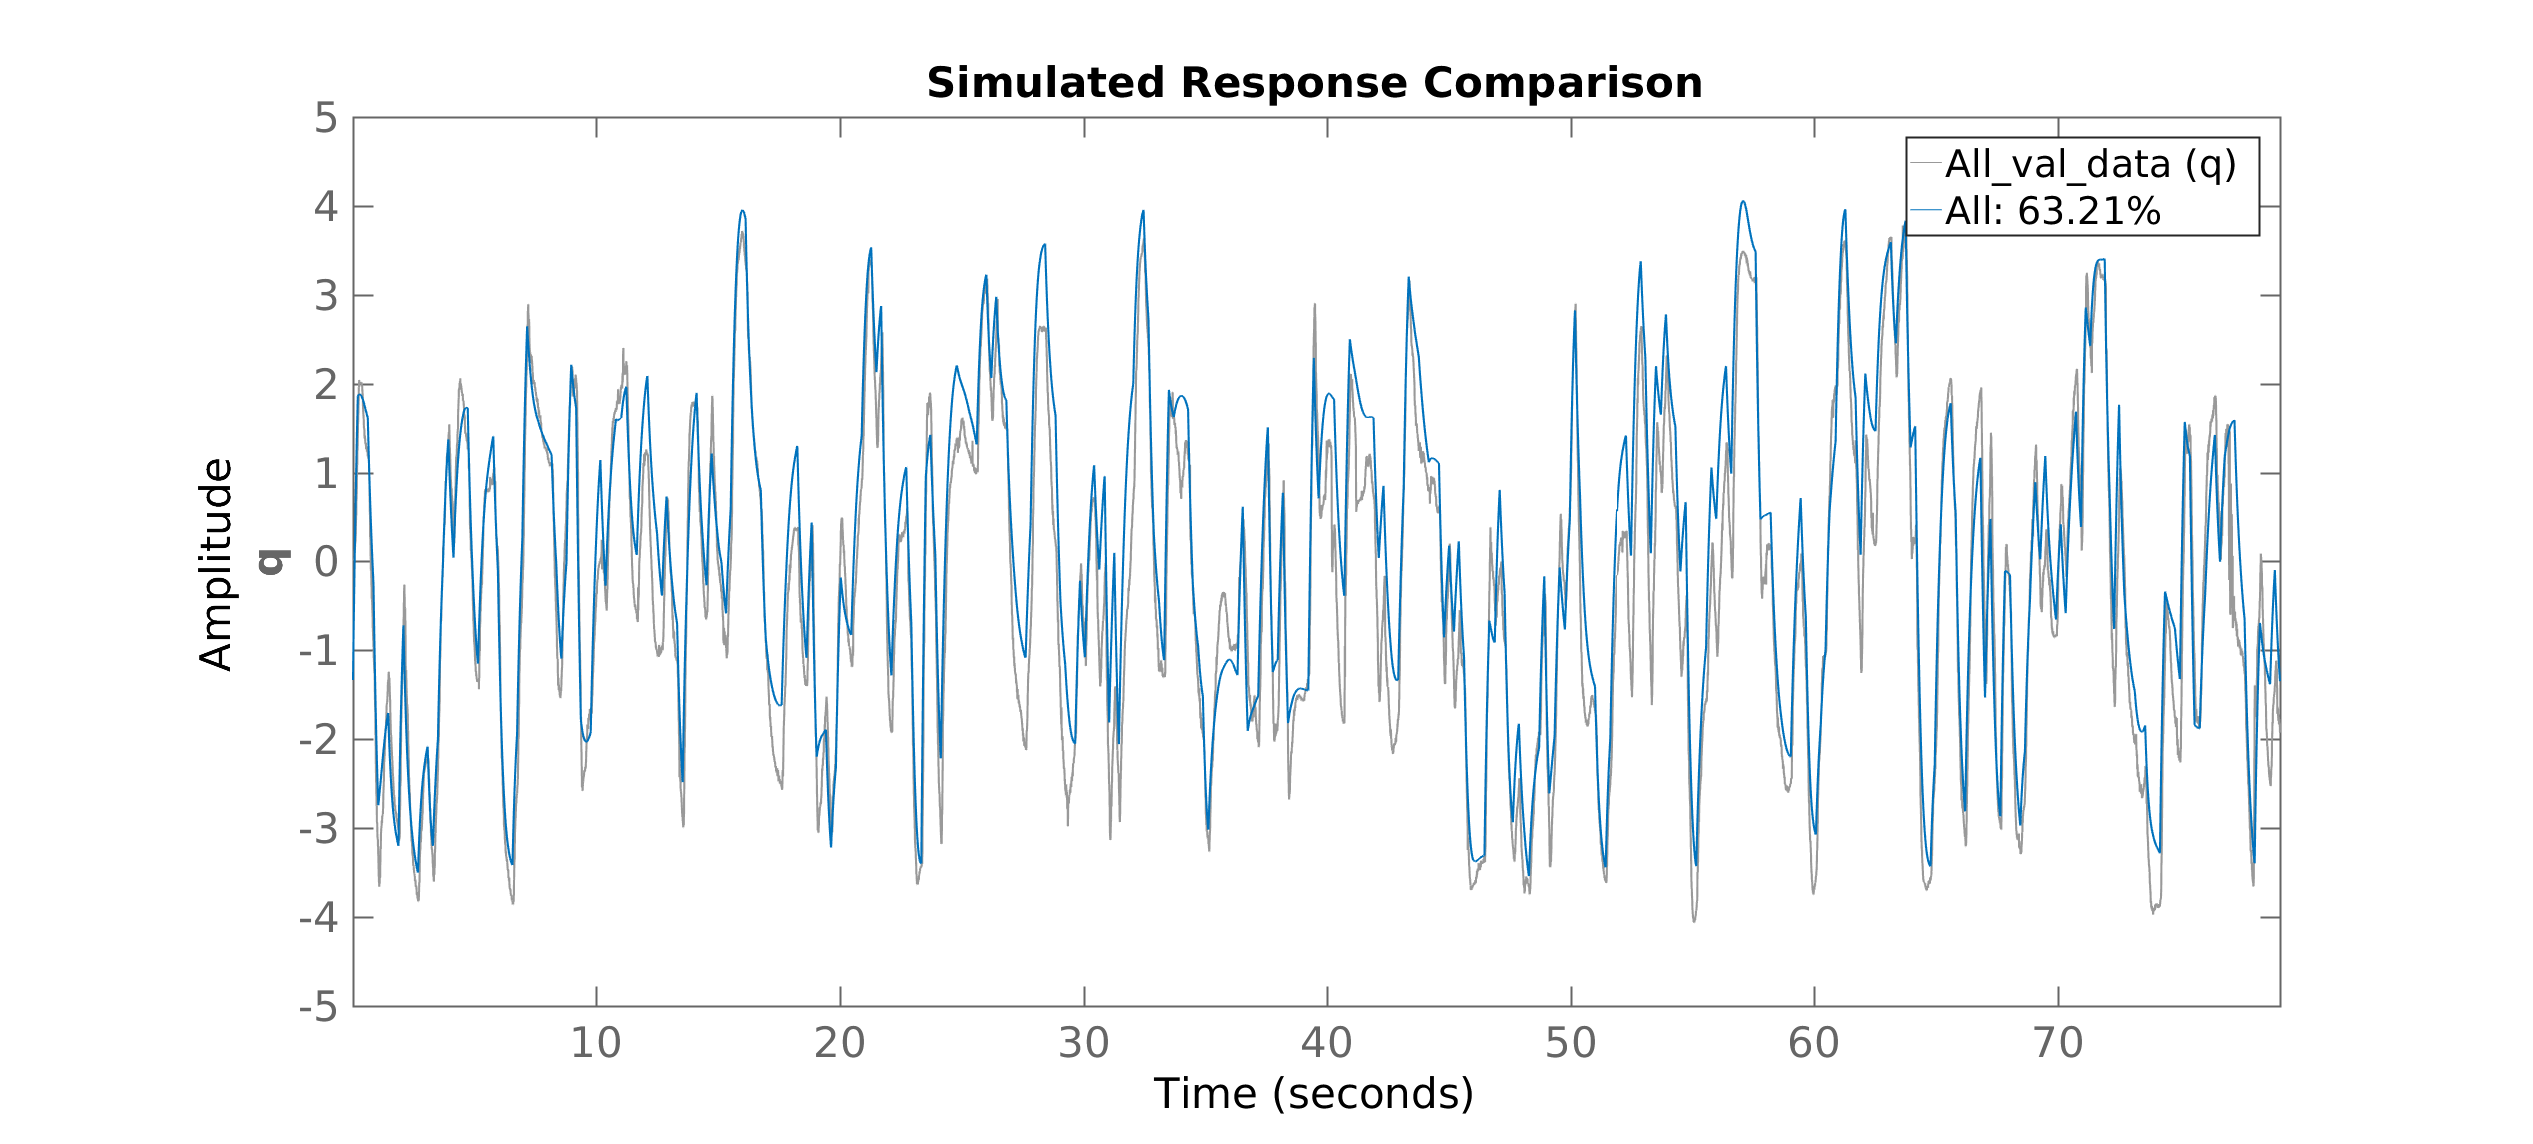
\includegraphics[width=0.4\textwidth]{velocityCompareq}}
  \caption{\label{fig:StepAllRate}% 
  }
\end{figure}

\begin{figure}[tbp]
  \centering
  \subfloat[][\label{fig:testSinP} An step was applied to $\rollVelocity$ .]{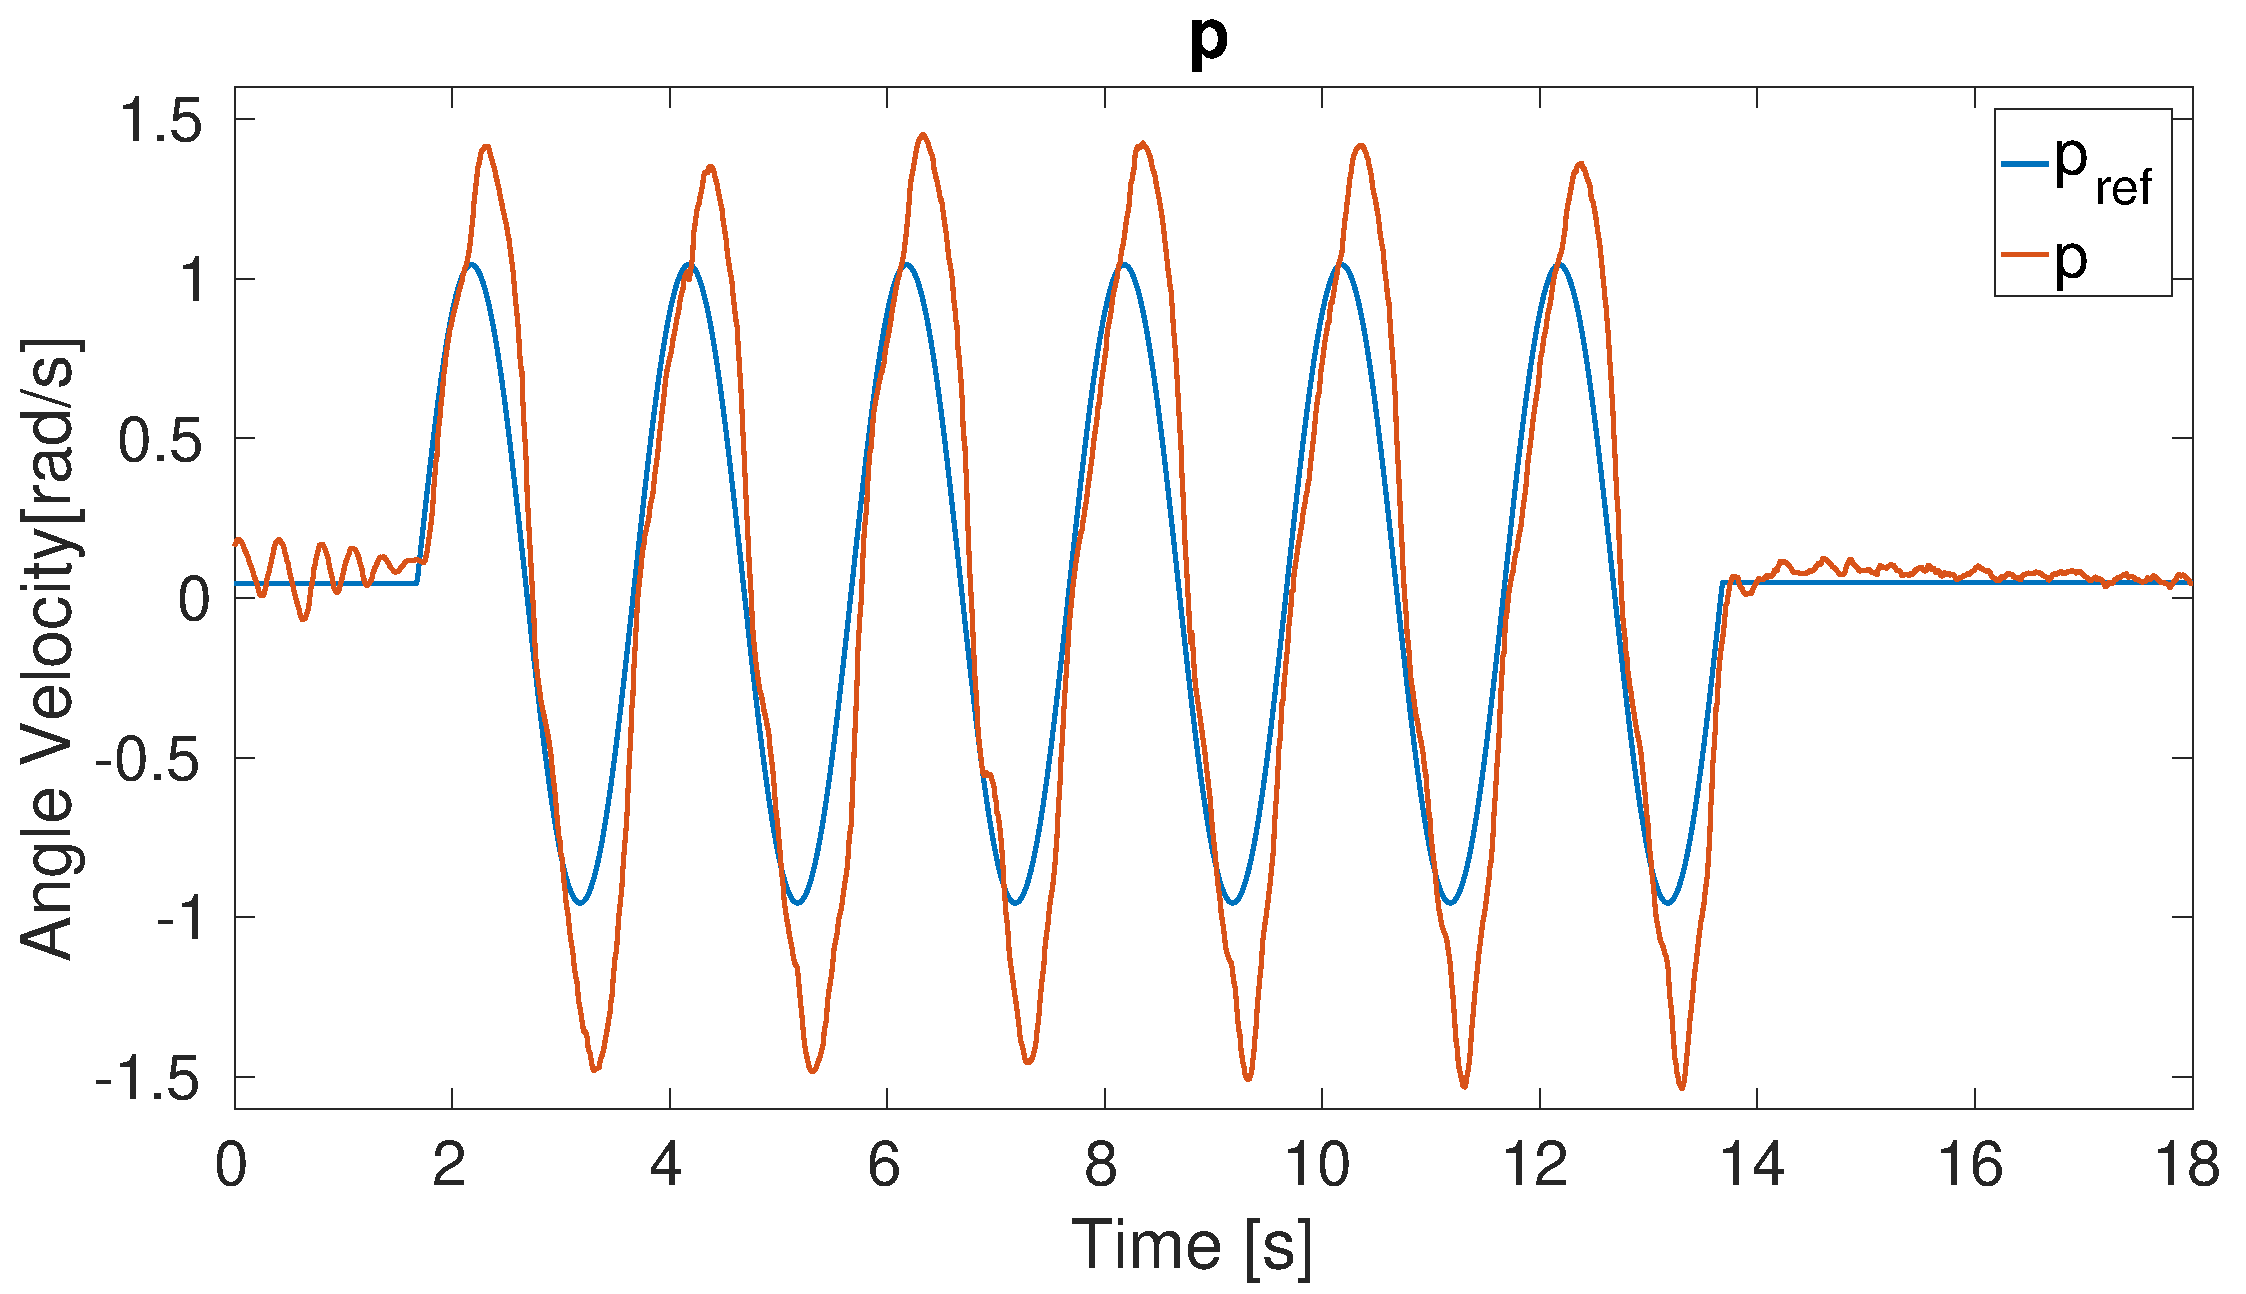
\includegraphics[width=0.4\textwidth]{testSinPA1}}
  \qquad
  \subfloat[][\label{fig:simSinP} An step was applied to the simulated \abbrROV in $\rollVelocity$.]{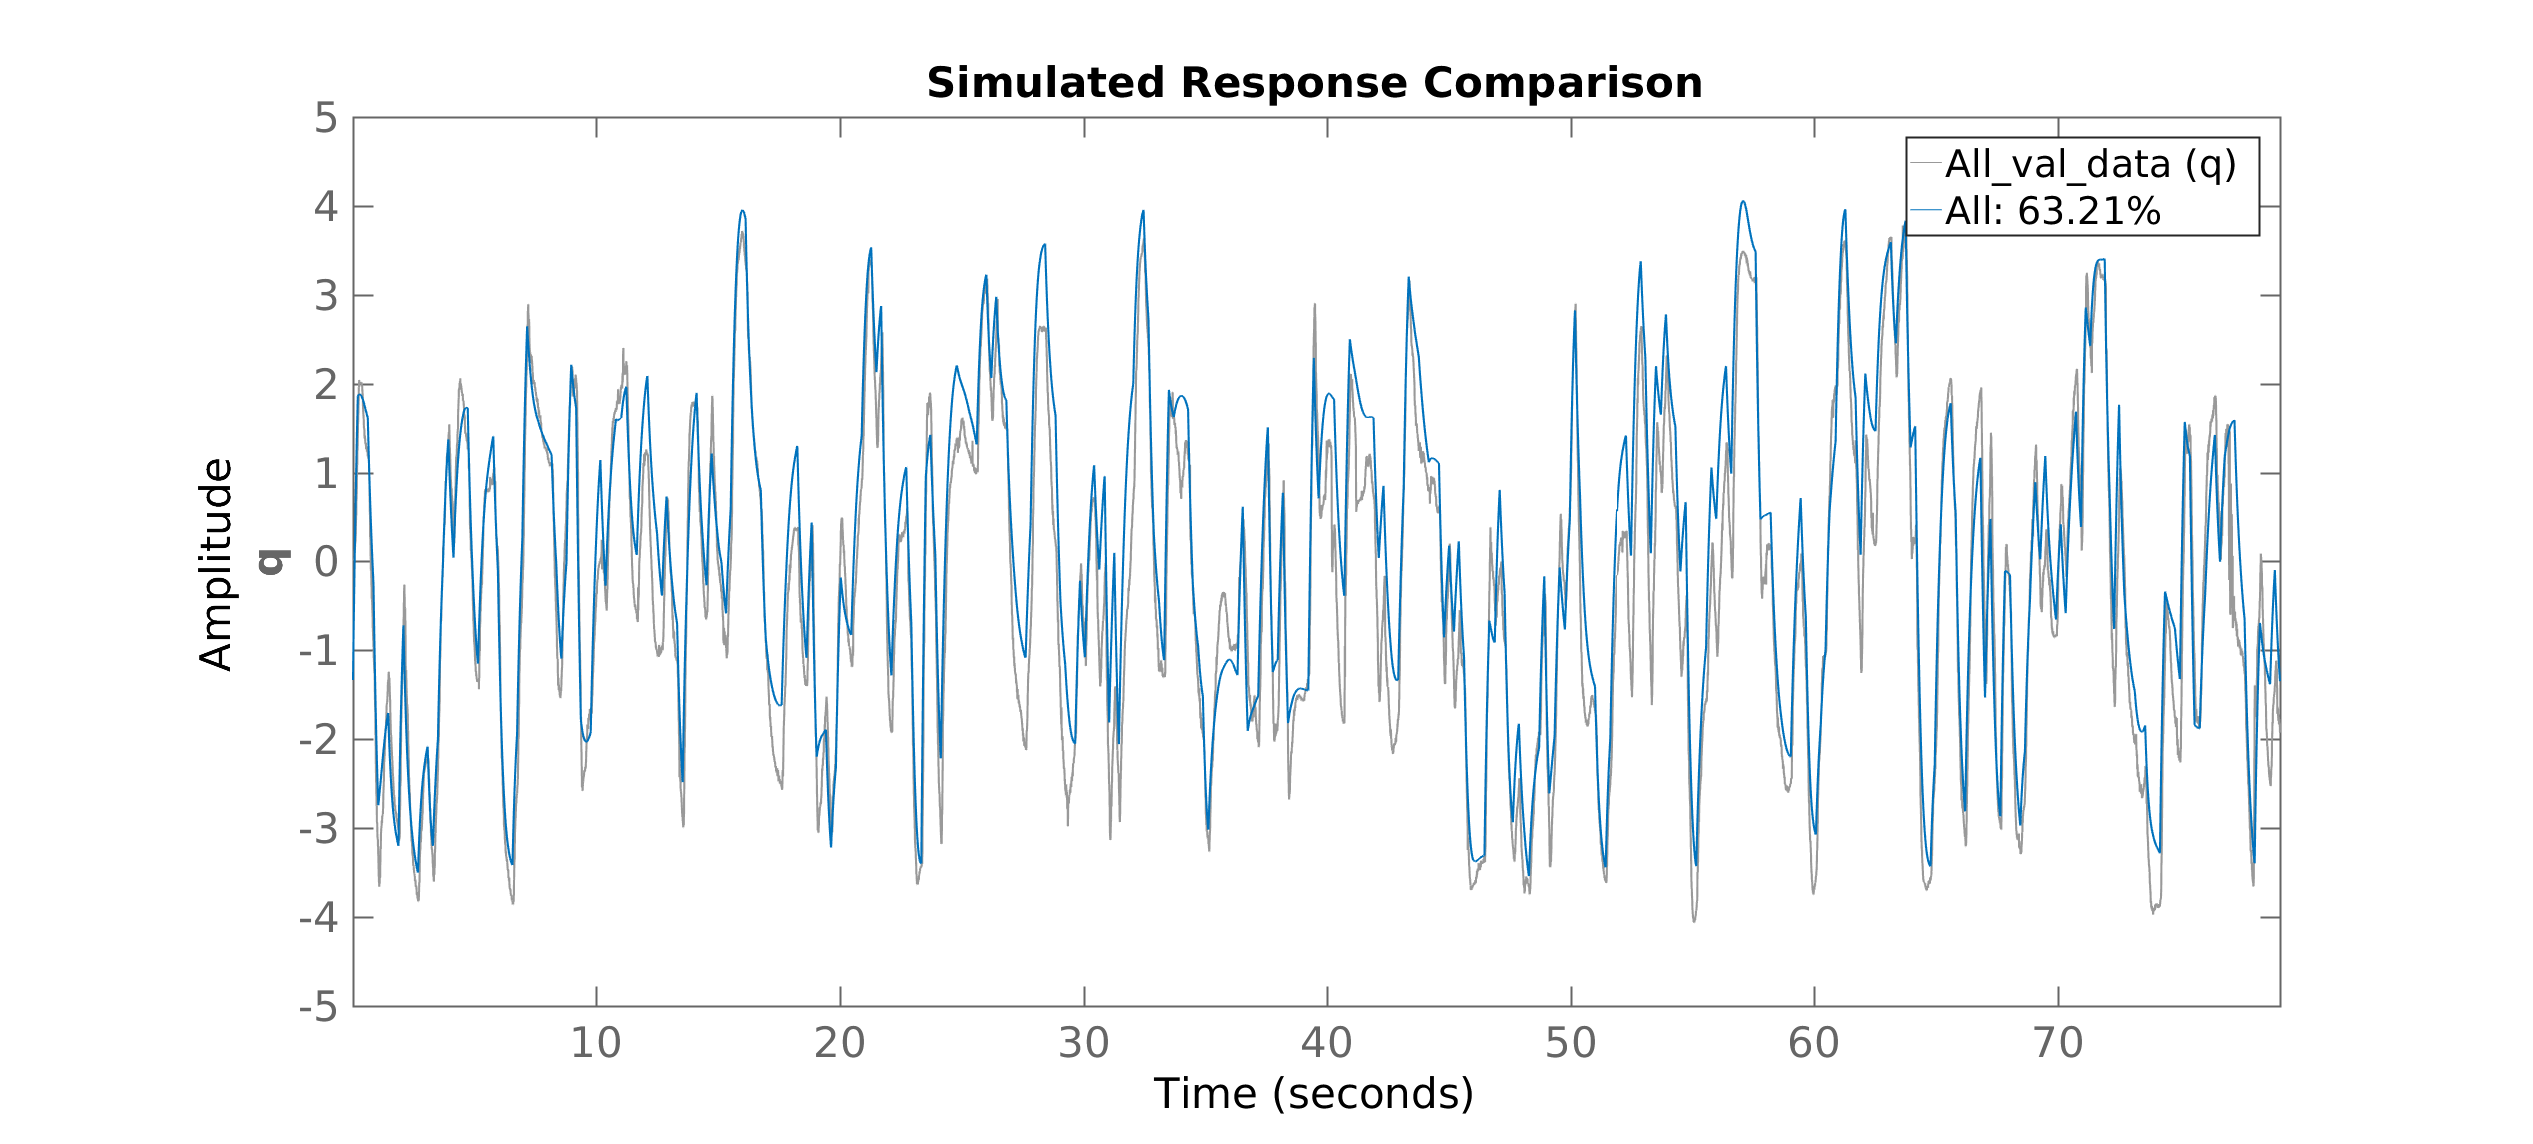
\includegraphics[width=0.4\textwidth]{velocityCompareq}}
  \qquad
  \subfloat[][\label{fig:testSinQ} An step was applied to $\pitchVelocity$ .]{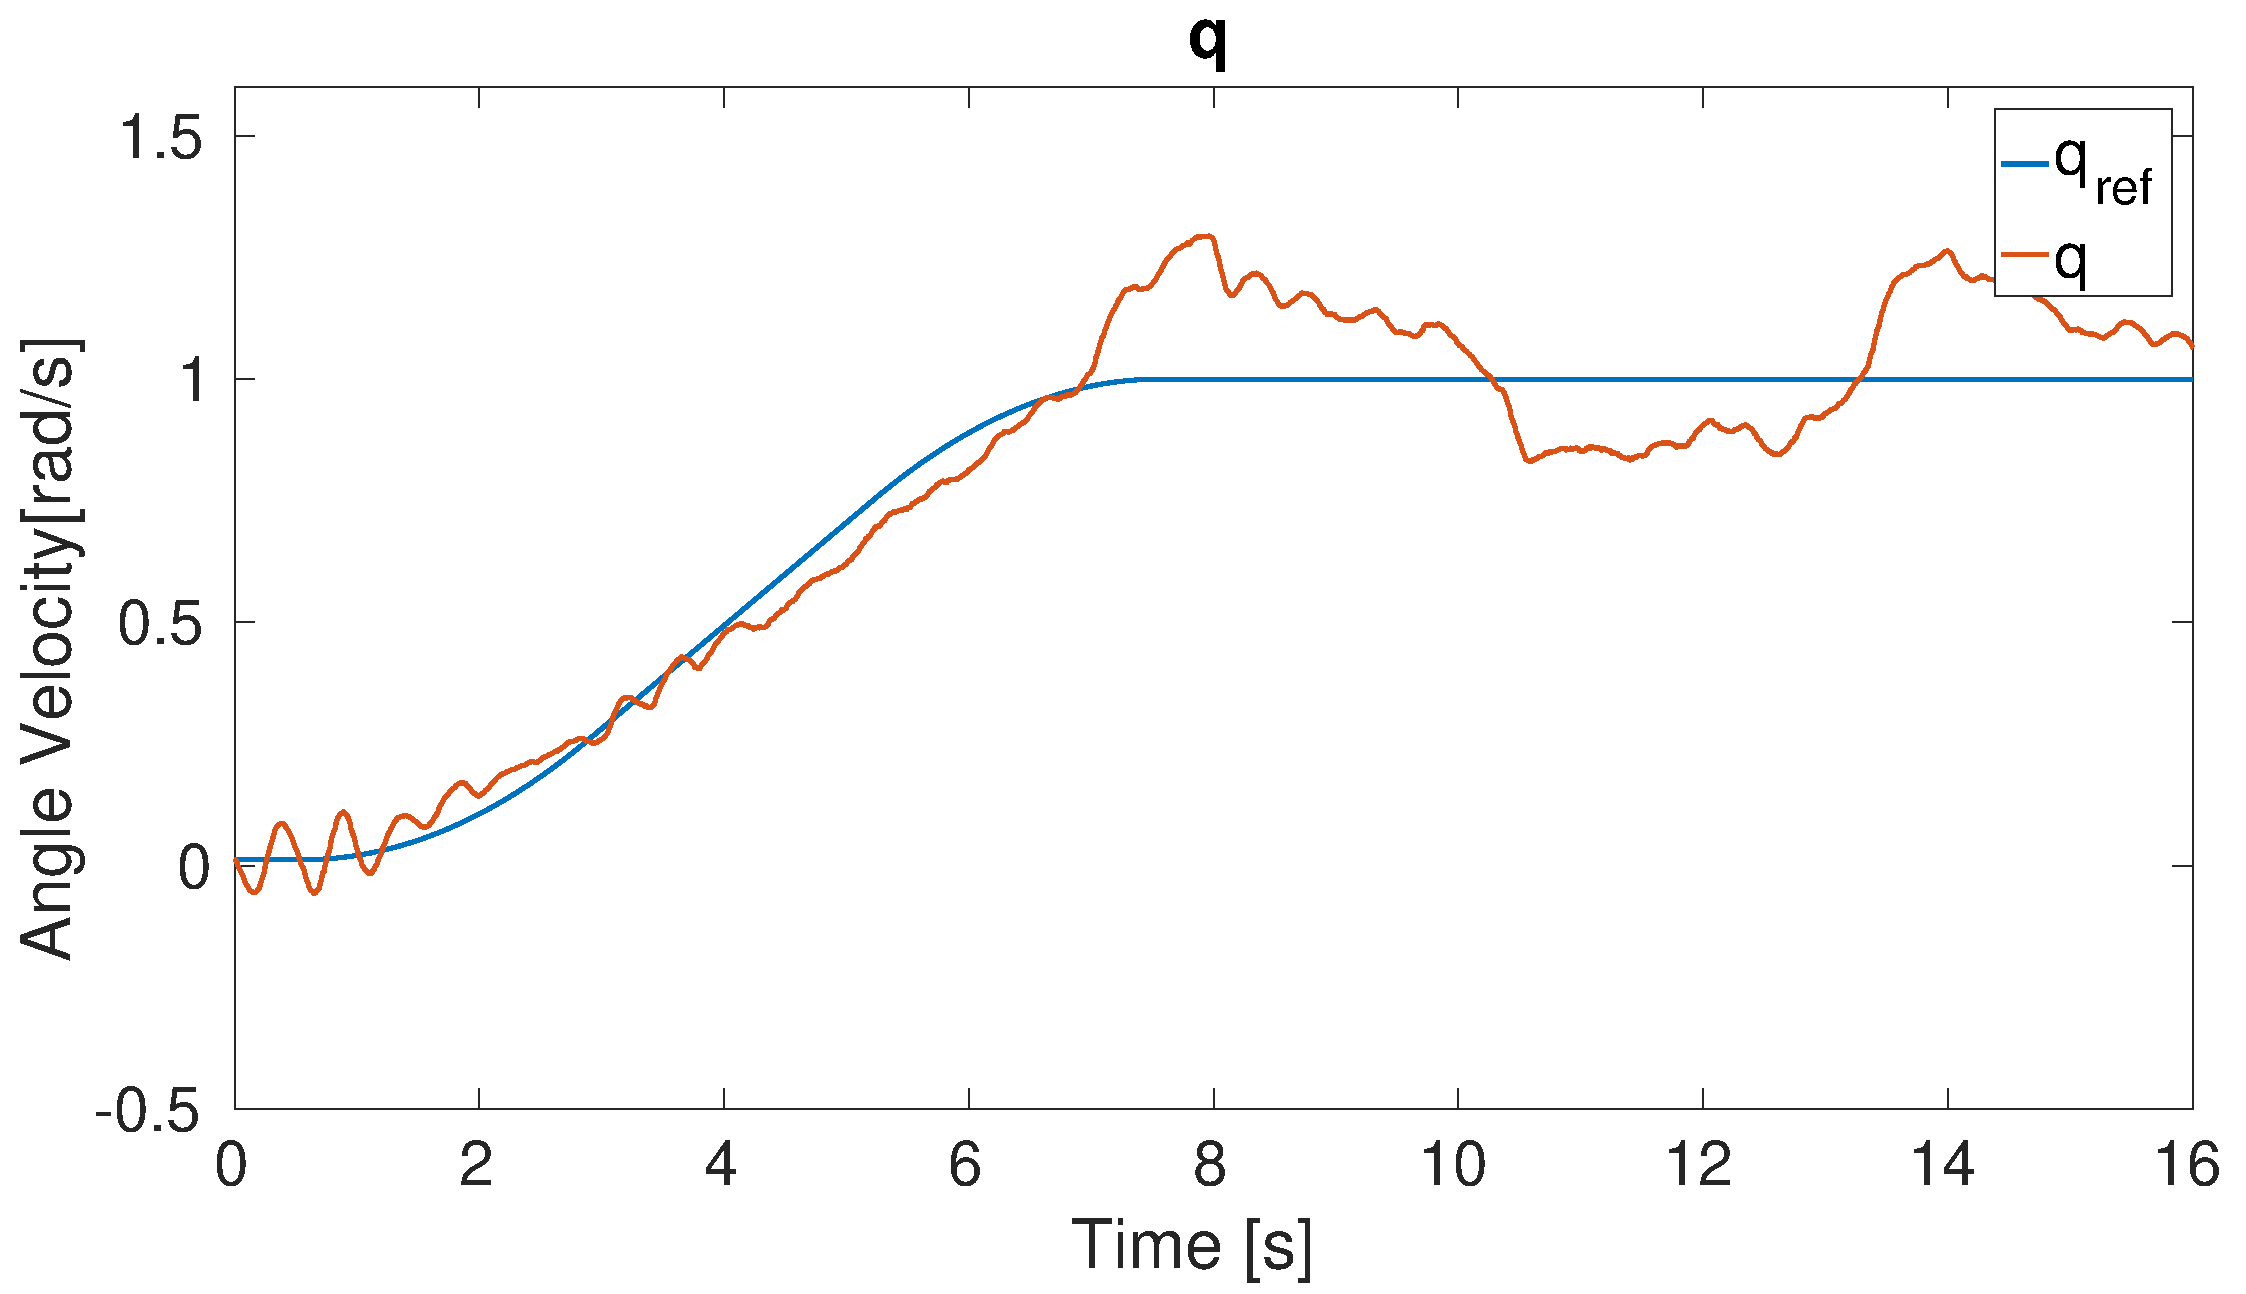
\includegraphics[width=0.4\textwidth]{testStepQs3e10a1}}
  \qquad
  \subfloat[][\label{fig:simSinQ} An step was applied to the simulated \abbrROV in $\pitchVelocity$.]{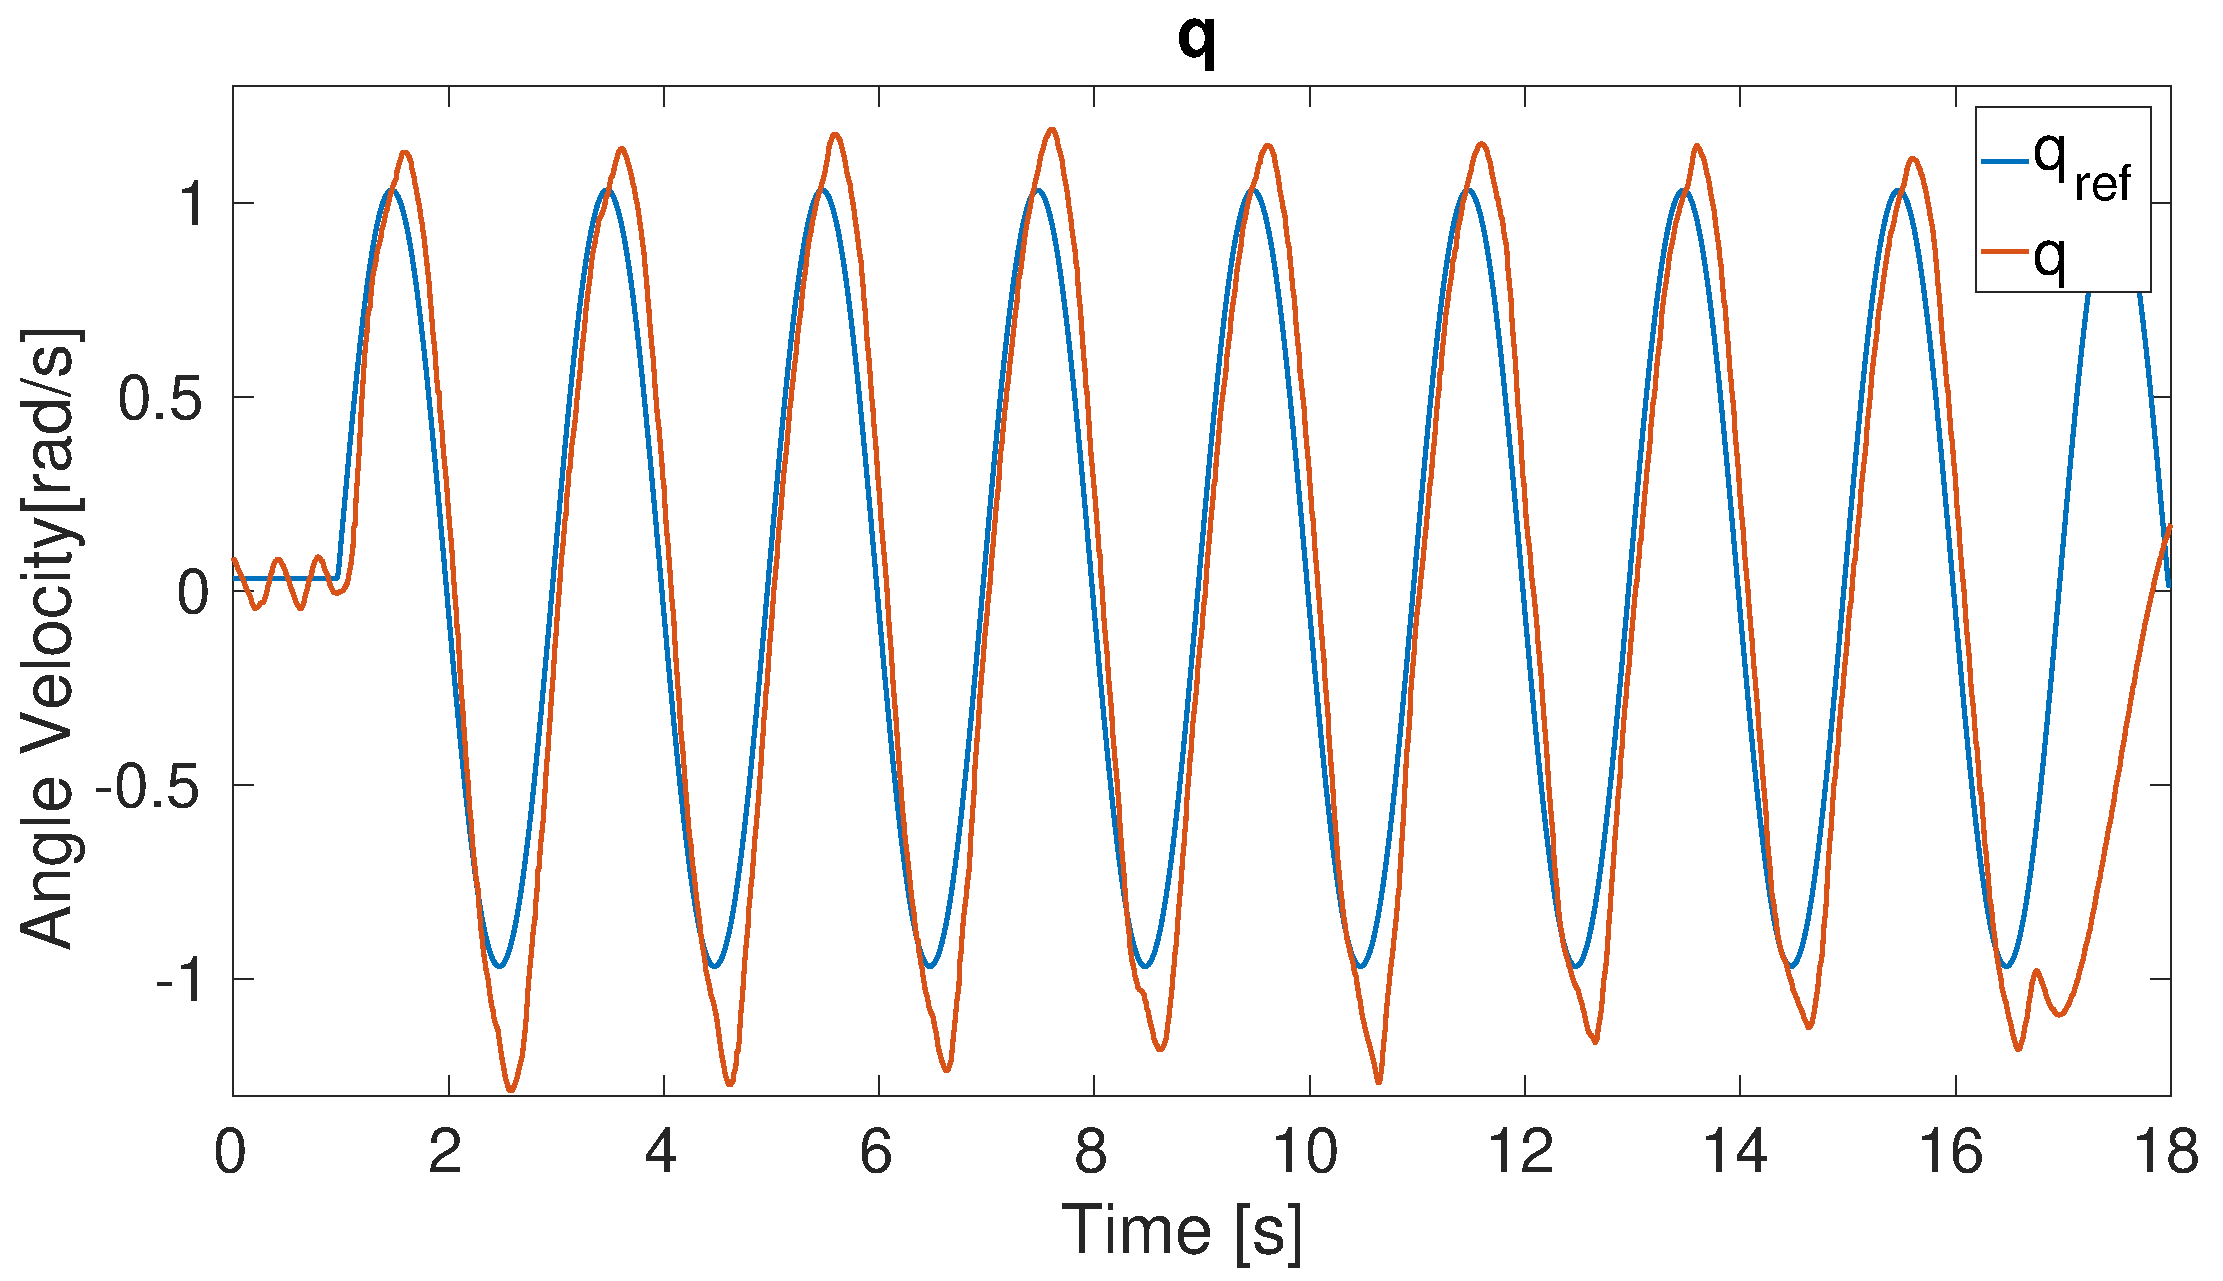
\includegraphics[width=0.4\textwidth]{testSinQA1}}
  \qquad
  \subfloat[][\label{fig:testSinR} An step was applied to $\yawVelocity$ .]{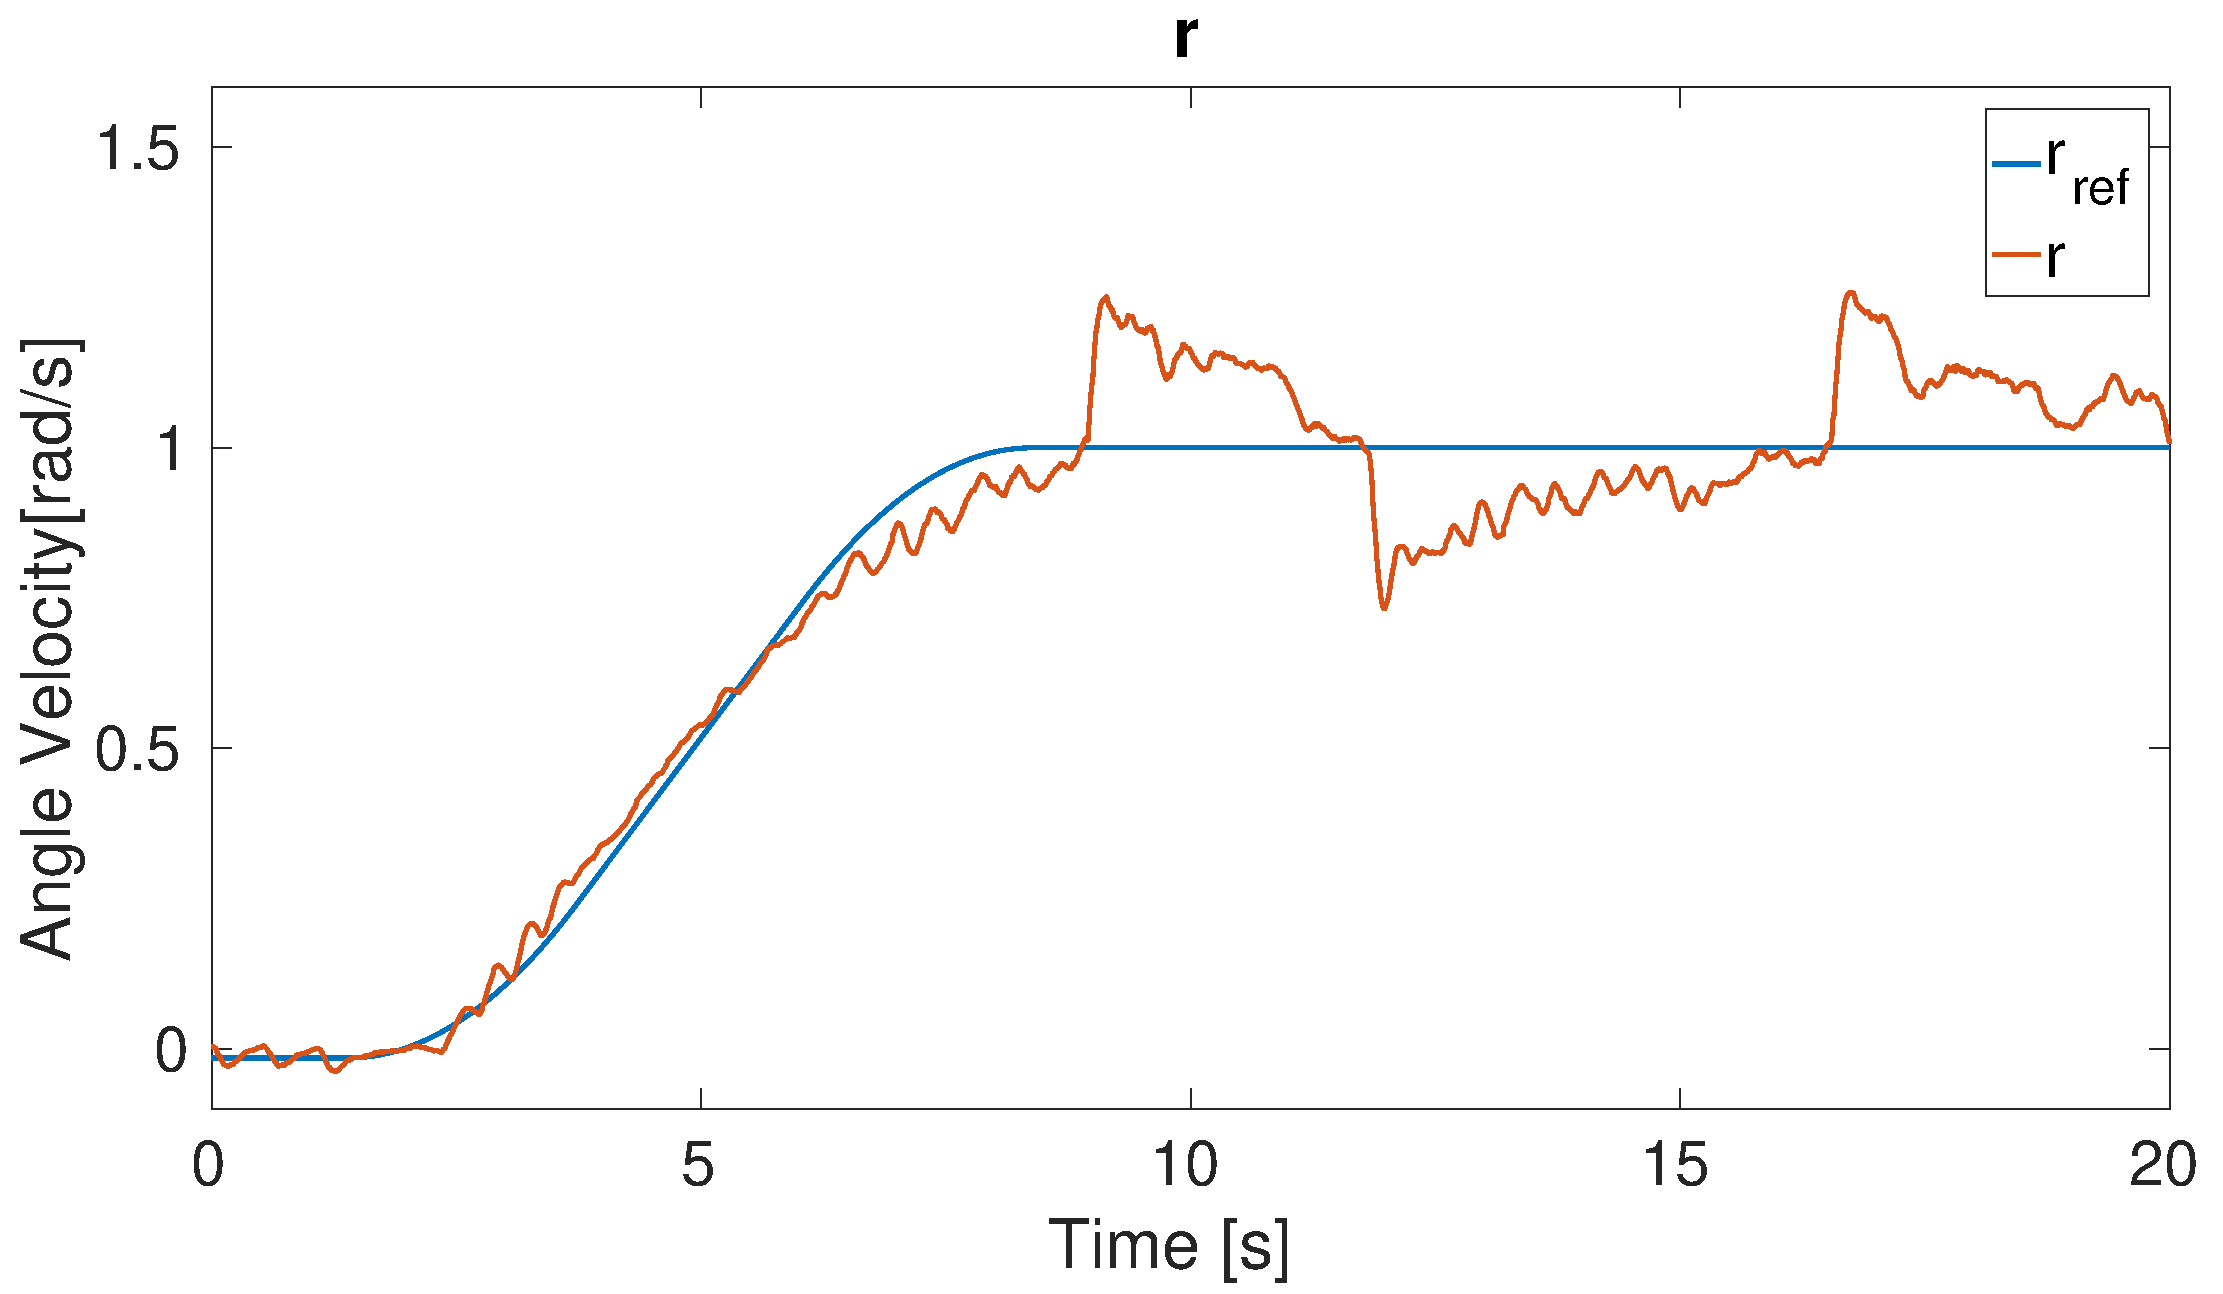
\includegraphics[width=0.4\textwidth]{testStepRs3e10a1}}
  \qquad
  \subfloat[][\label{fig:simSinR} An step was applied to the simulated \abbrROV in $\yawVelocity$.]{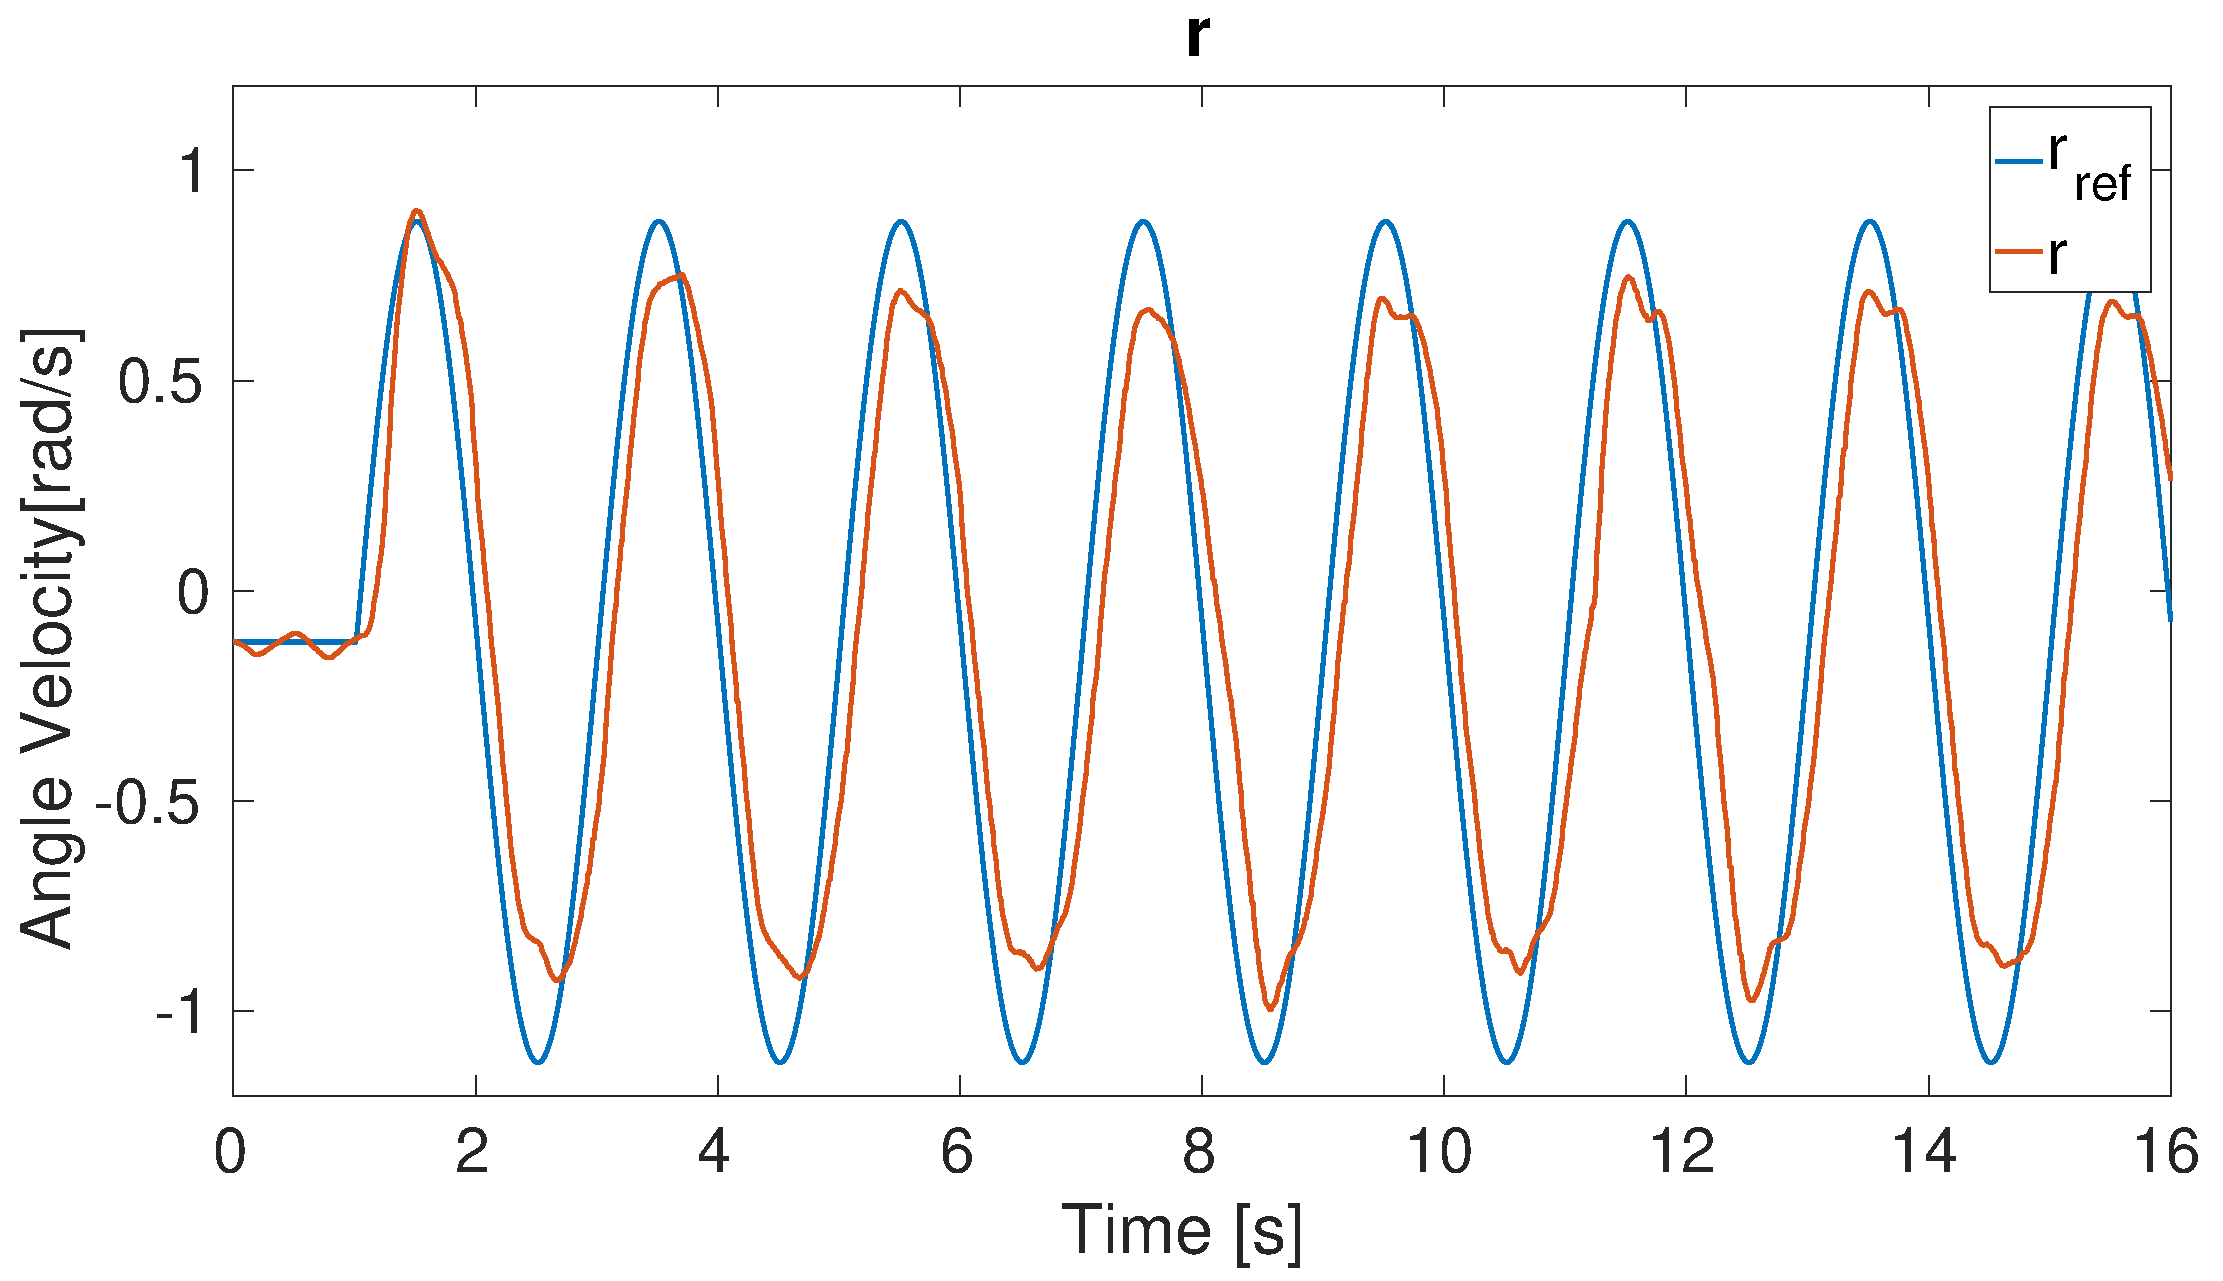
\includegraphics[width=0.4\textwidth]{testSinRA1}}
    \caption{\label{fig:Sin1Rate}% 
    Comparison between simulation and a real test of a smooth step reference in.}
\end{figure}

\begin{figure}
\centering
  \subfloat[][\label{fig:testSinAllPRate} An step was applied to all \abbrDOF.]{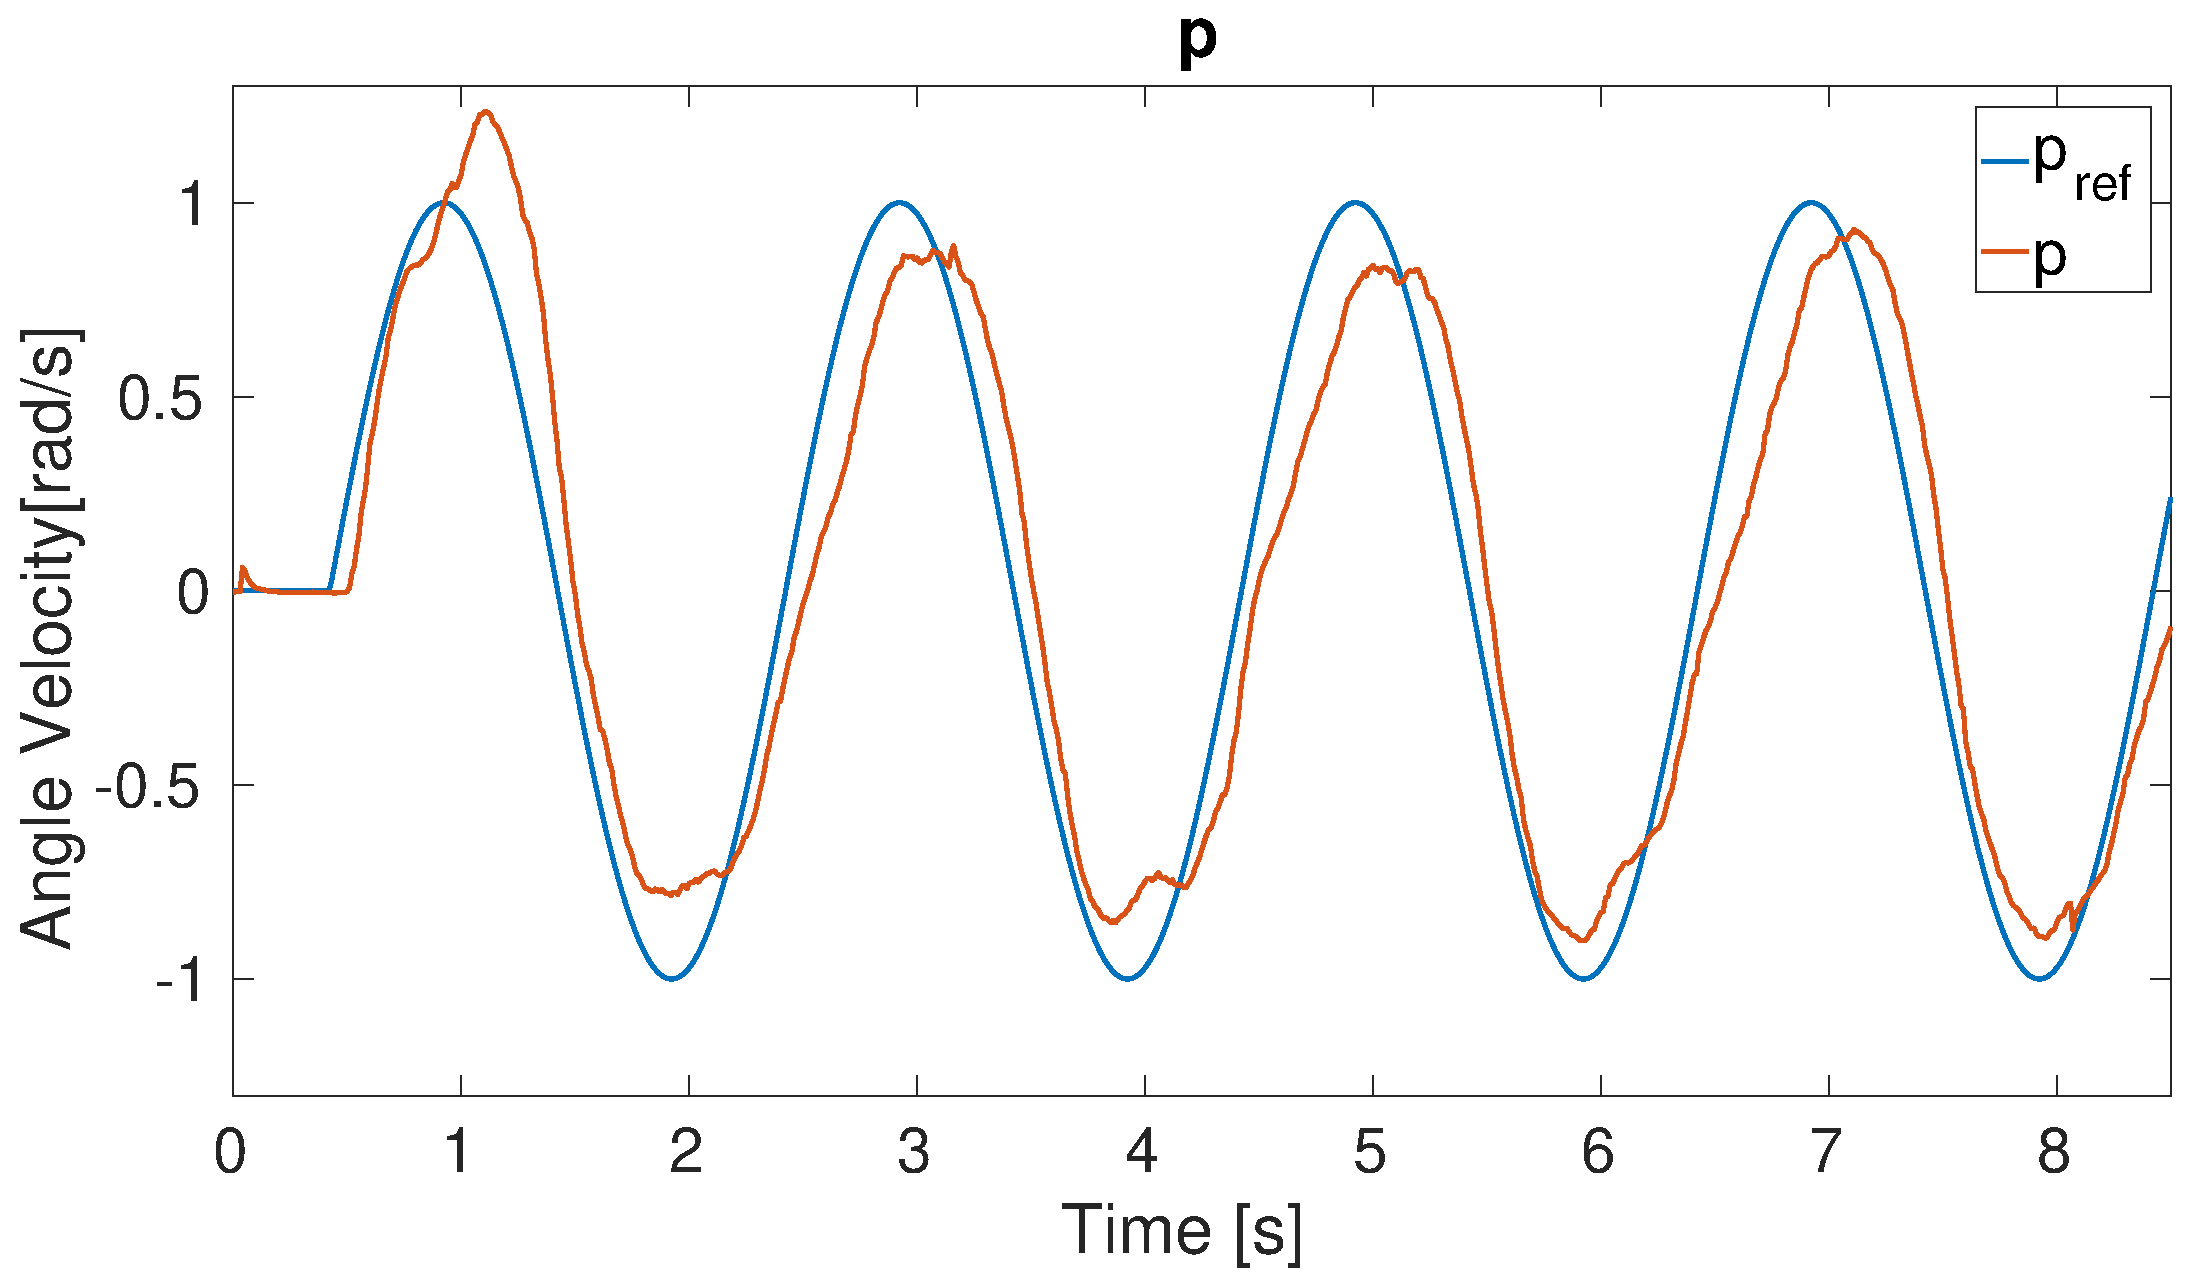
\includegraphics[width=0.4\textwidth]{testSinAllPA1}}
  \qquad
  \subfloat[][\label{fig:simSinAllPRate} An step was applied to the simulated \abbrROV in all \abbrDOF.]{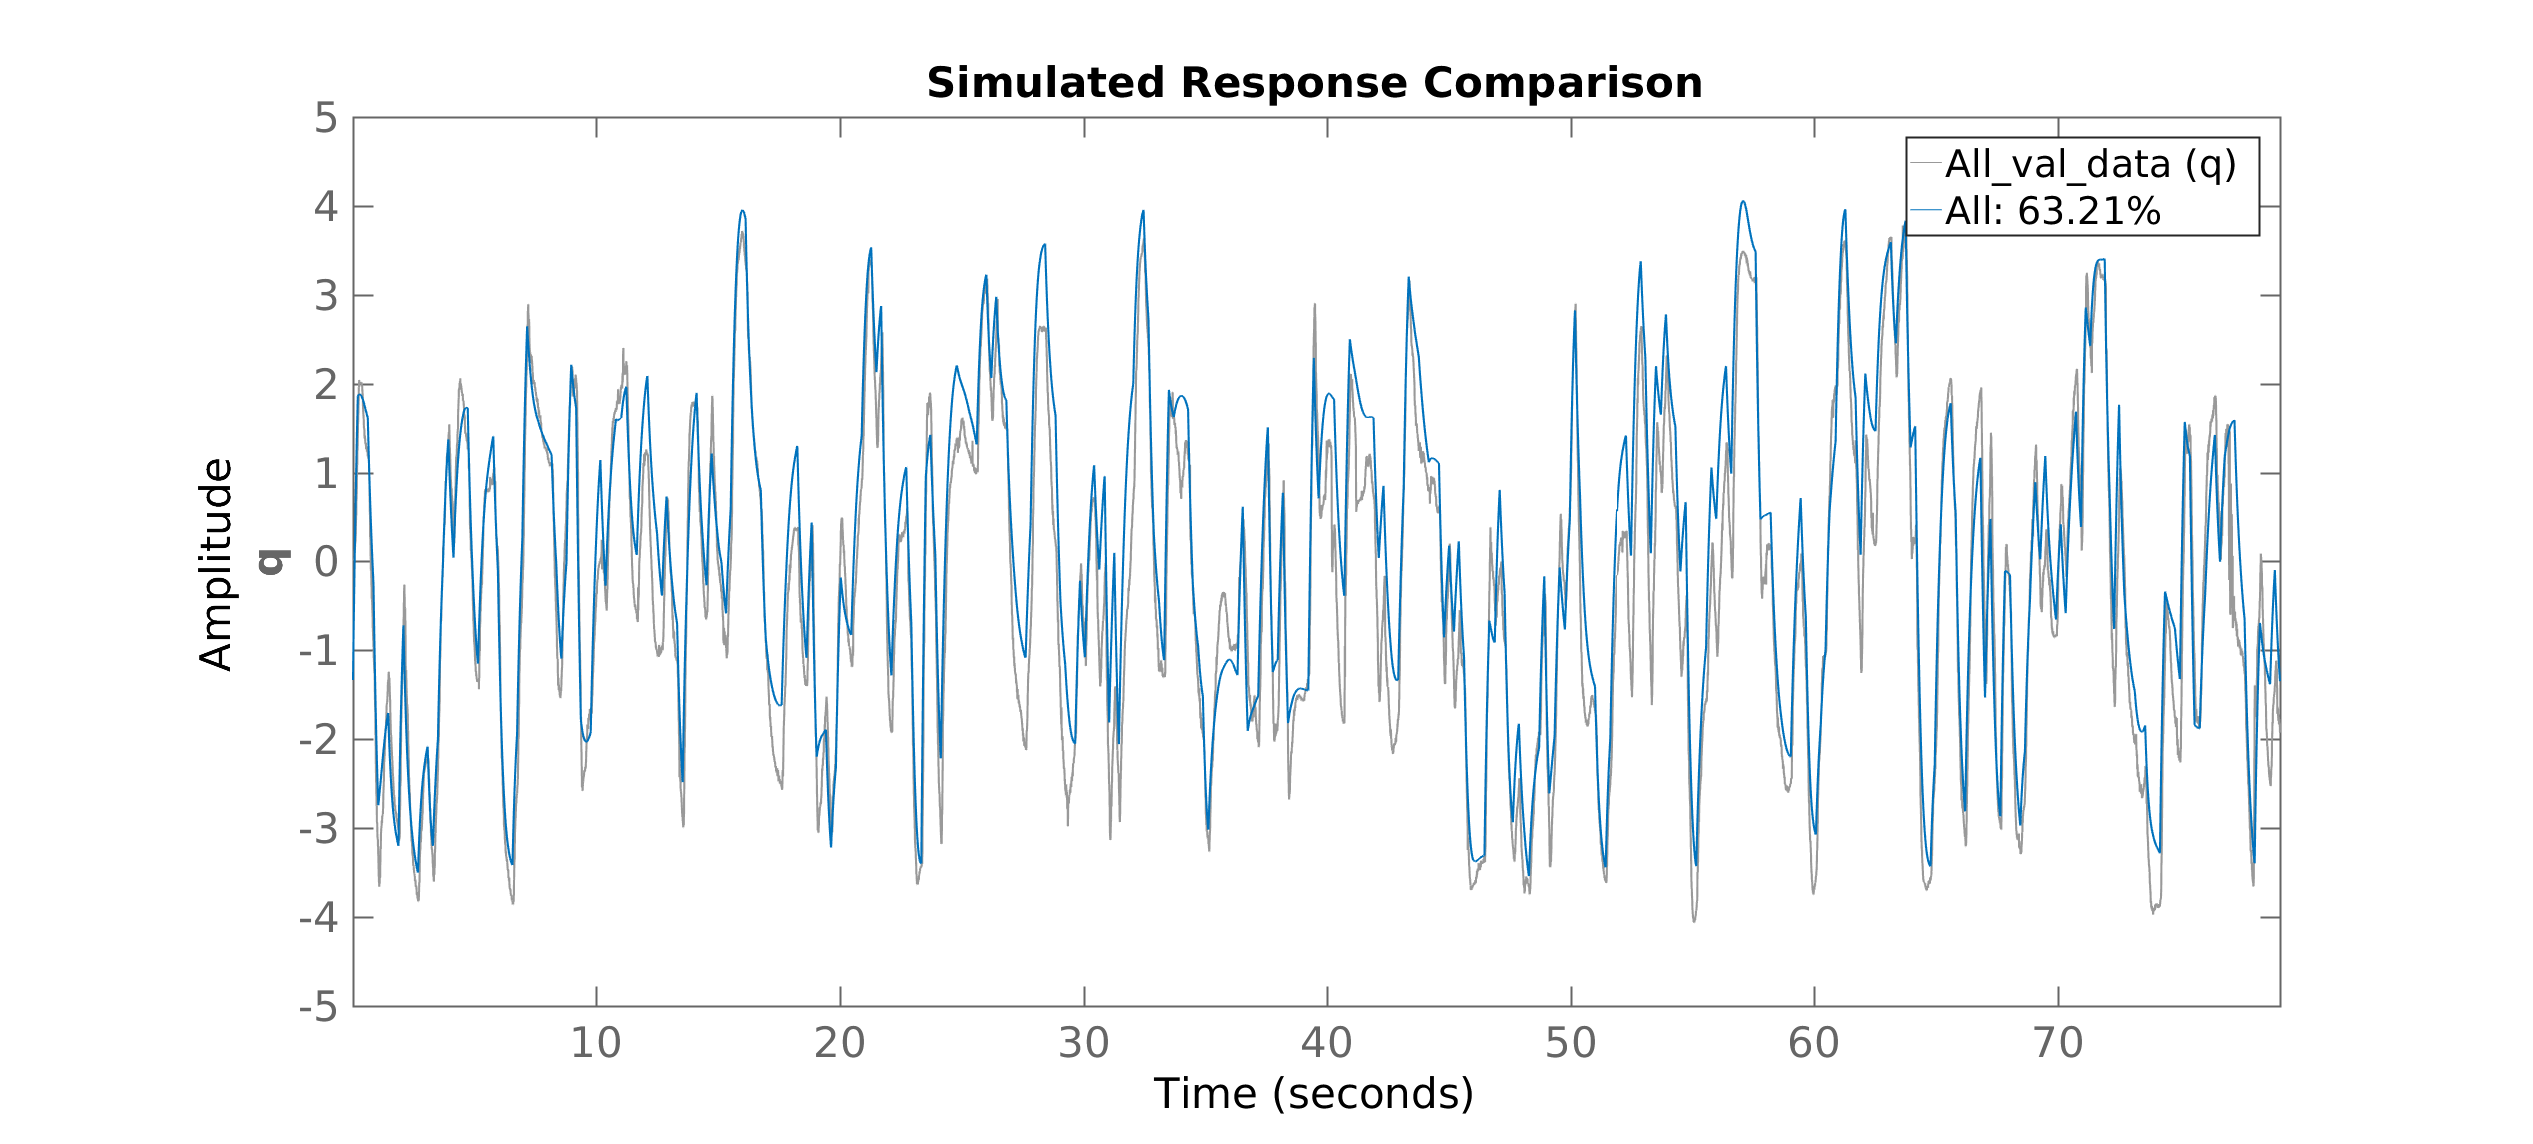
\includegraphics[width=0.4\textwidth]{velocityCompareq}}
  \qquad
  \subfloat[][\label{fig:testSinAllQRate} An step was applied to the simulated \abbrROV in all \abbrDOF.]{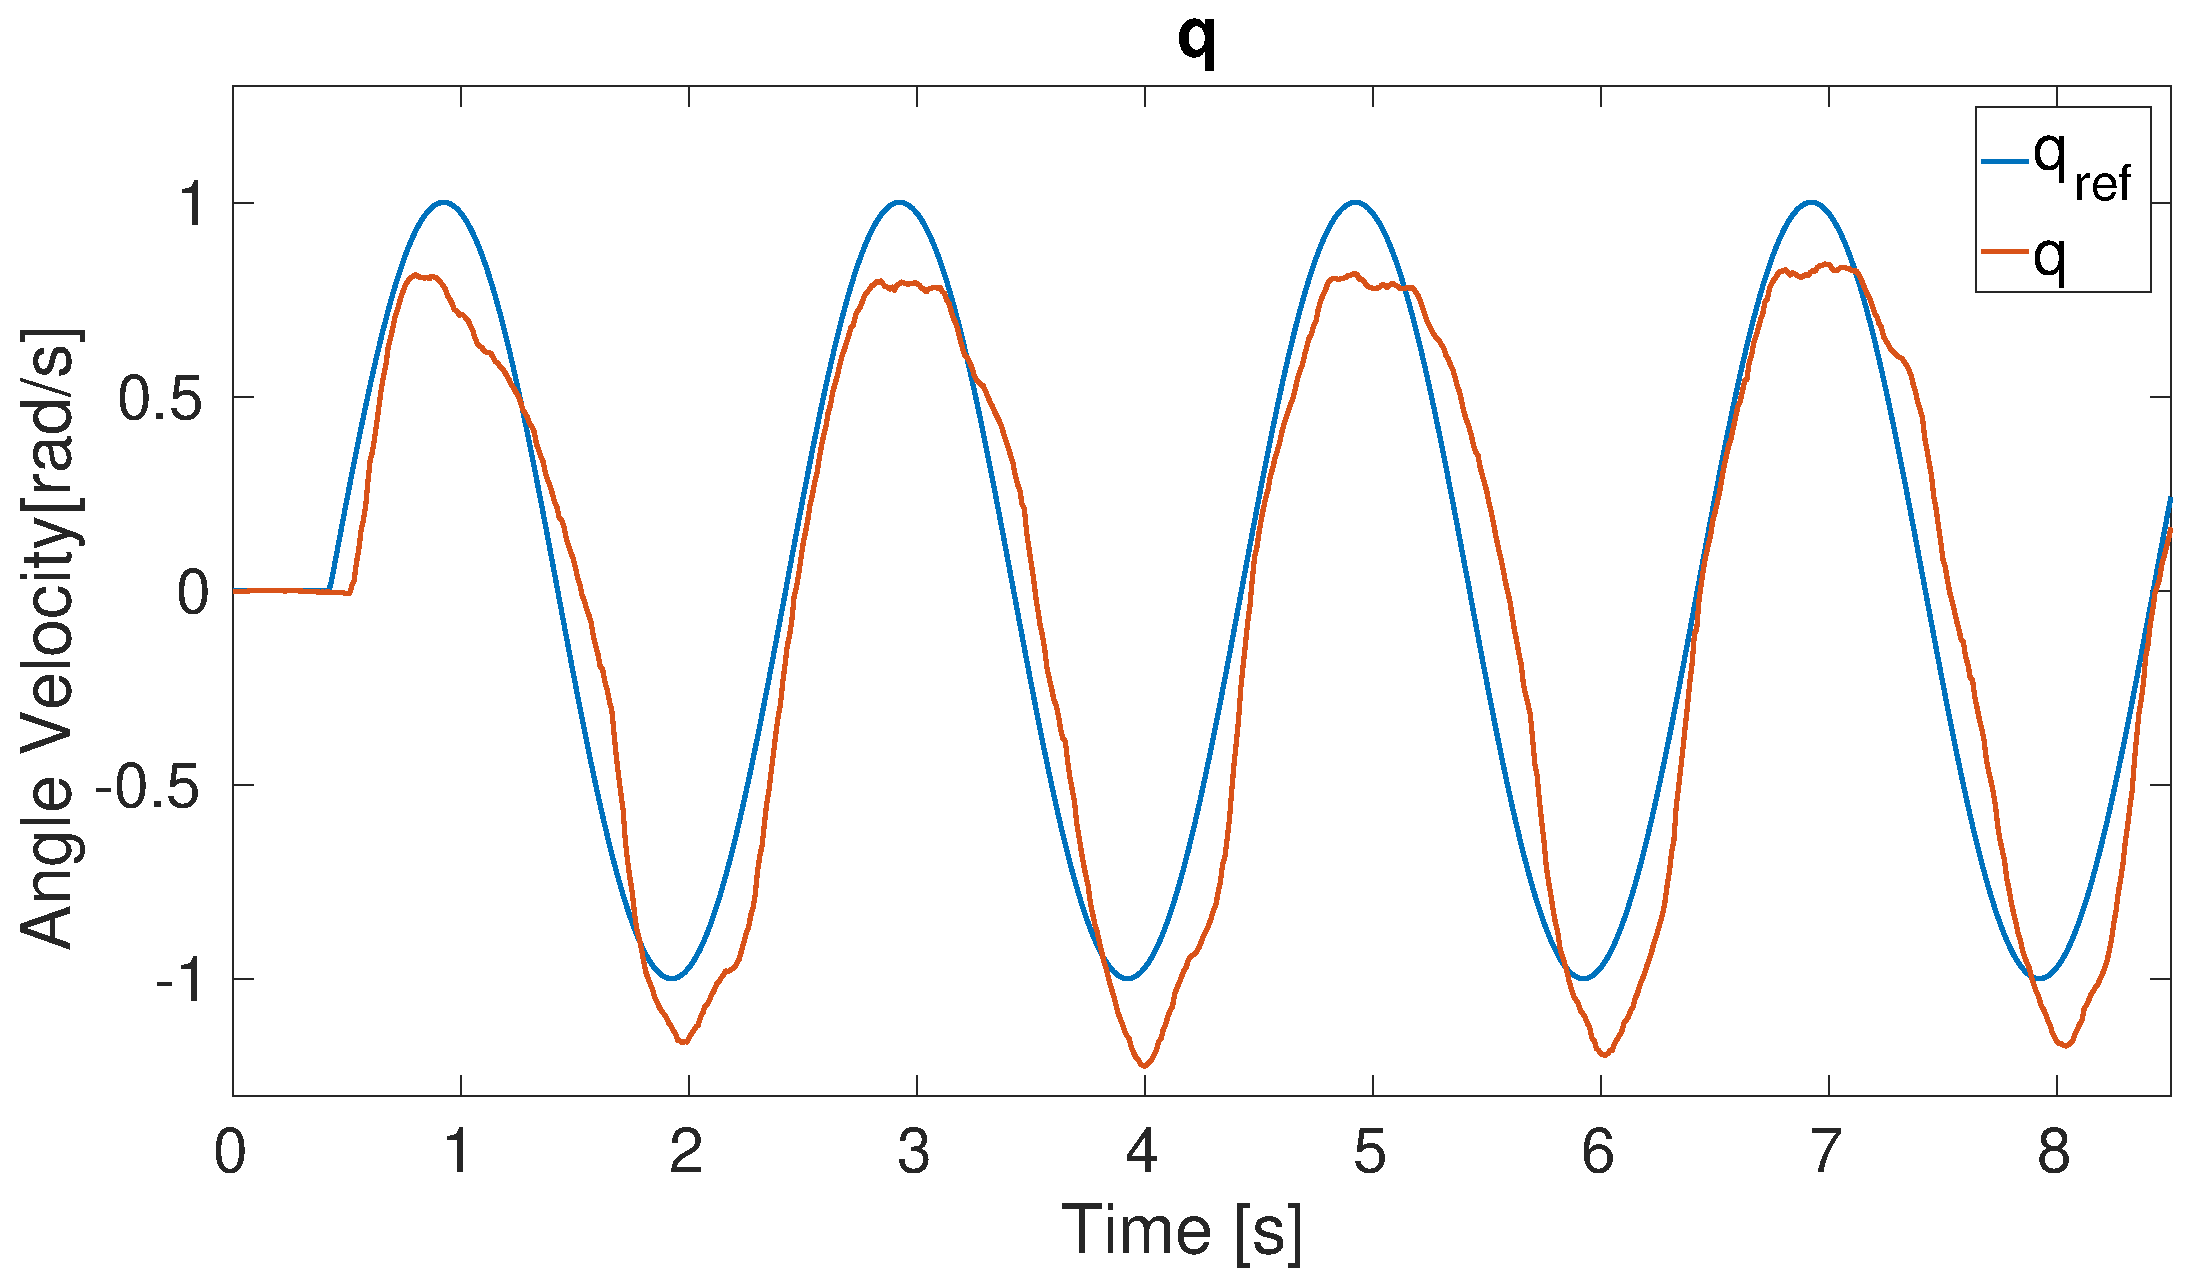
\includegraphics[width=0.4\textwidth]{testSinAllQA1}}
  \qquad
  \subfloat[][\label{fig:simSinAllQRate} An step was applied to the simulated \abbrROV in all \abbrDOF.]{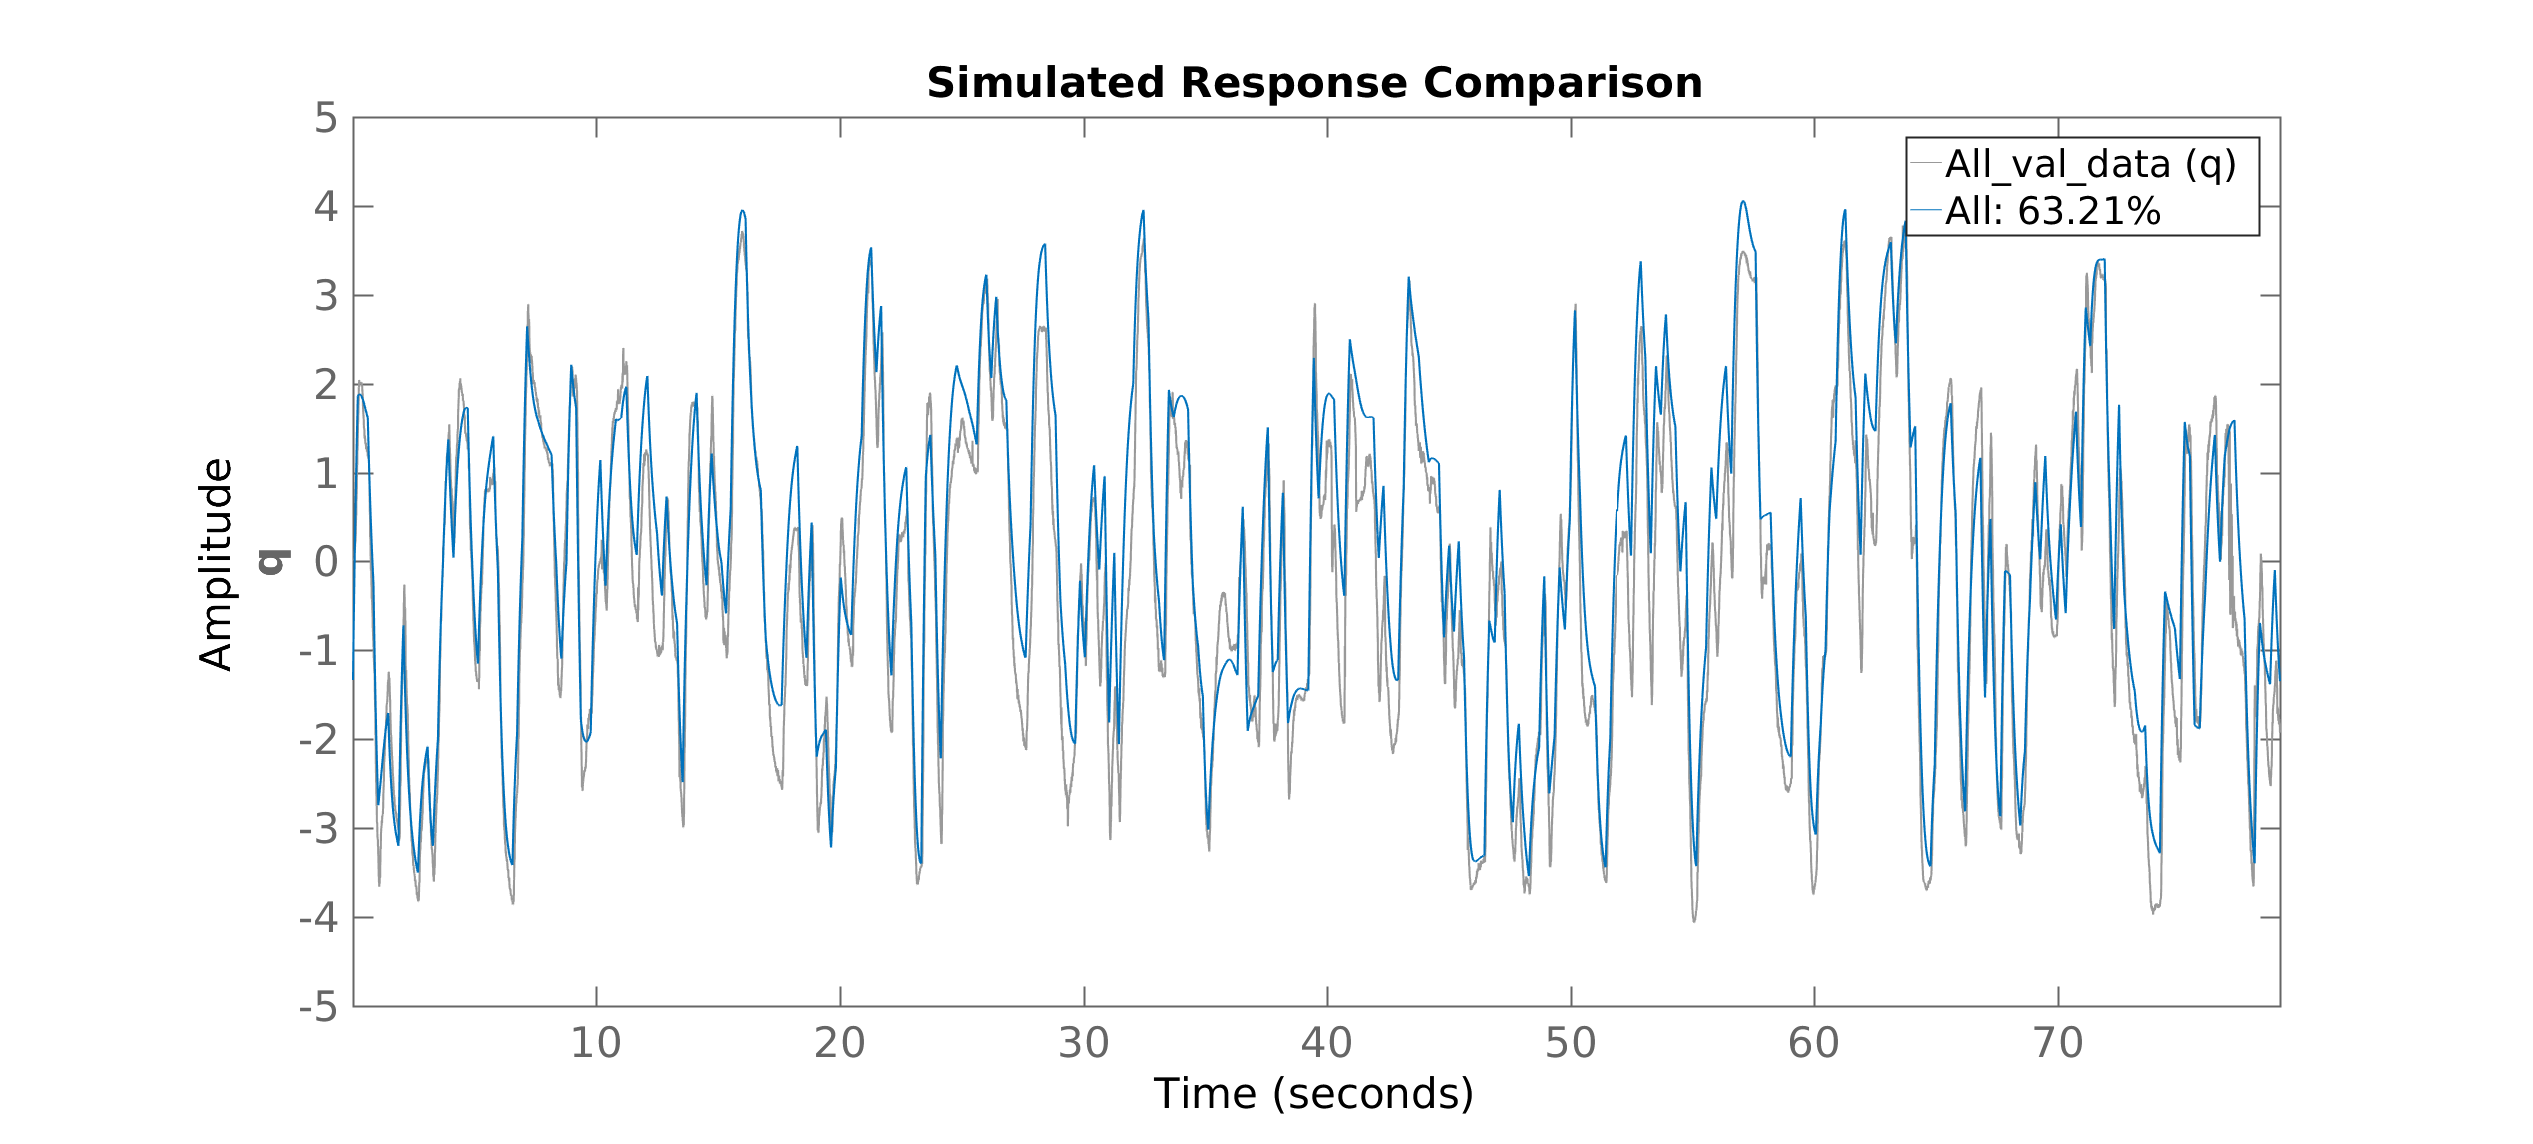
\includegraphics[width=0.4\textwidth]{velocityCompareq}}
  \qquad
  \subfloat[][\label{fig:testSinAllRRate} An step was applied to the simulated \abbrROV in all \abbrDOF.]{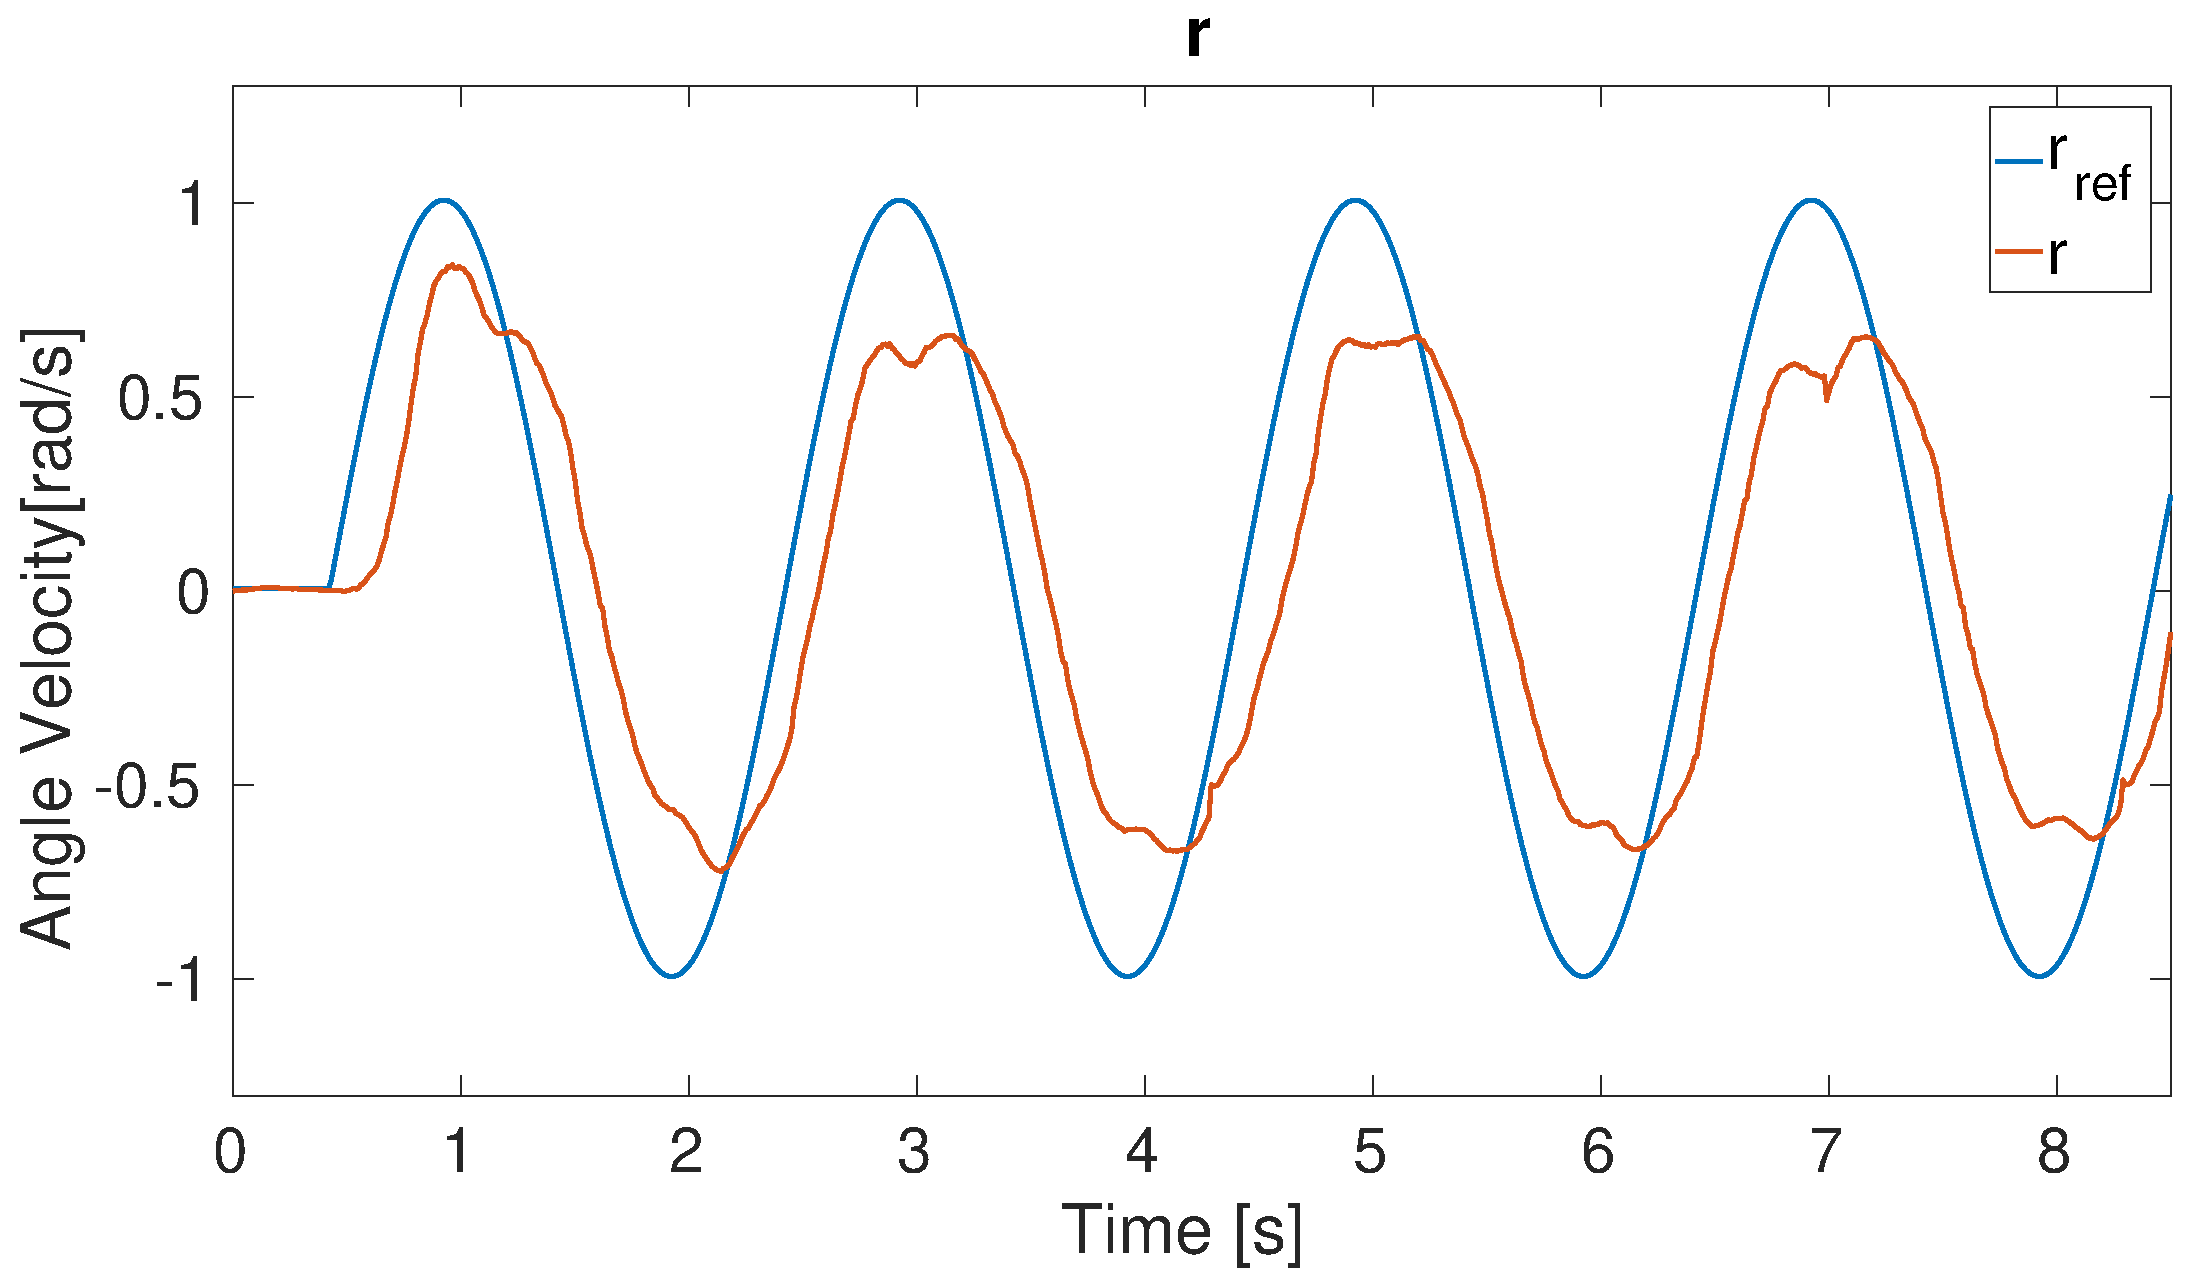
\includegraphics[width=0.4\textwidth]{testSinAllRA1}}
  \qquad
  \subfloat[][\label{fig:simSinAllRRate} An step was applied to the simulated \abbrROV in all \abbrDOF.]{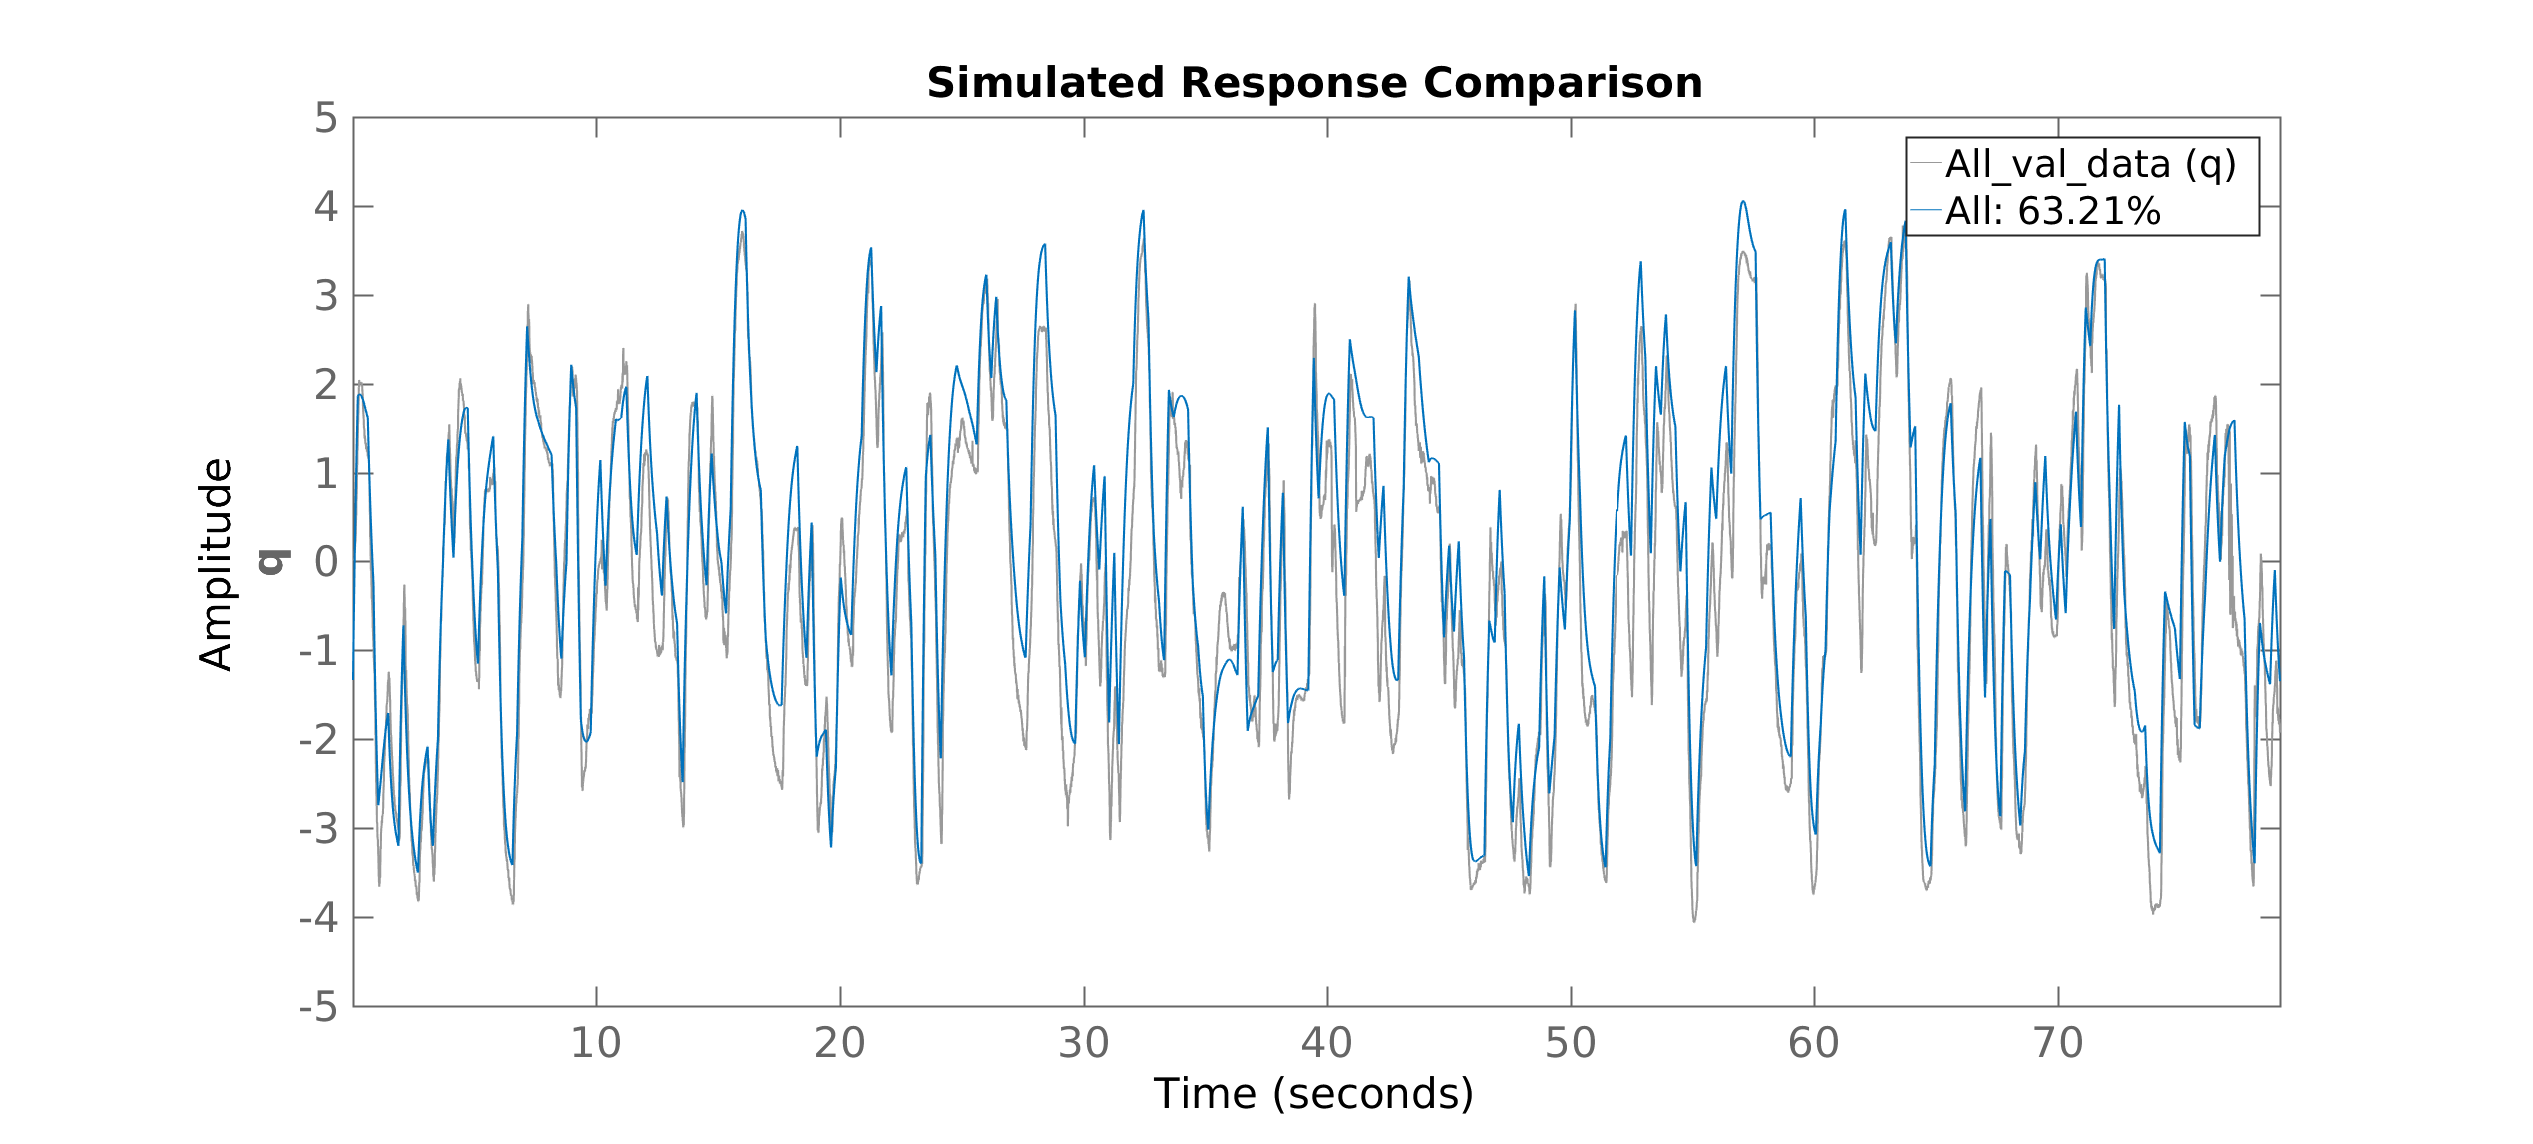
\includegraphics[width=0.4\textwidth]{velocityCompareq}}
  \caption{\label{fig:Sin1AllRate}%
  }
\end{figure}


\begin{figure}[tbp]
  \centering
  \subfloat[][\label{fig:testSin05P} An step was applied to $\rollVelocity$ .]{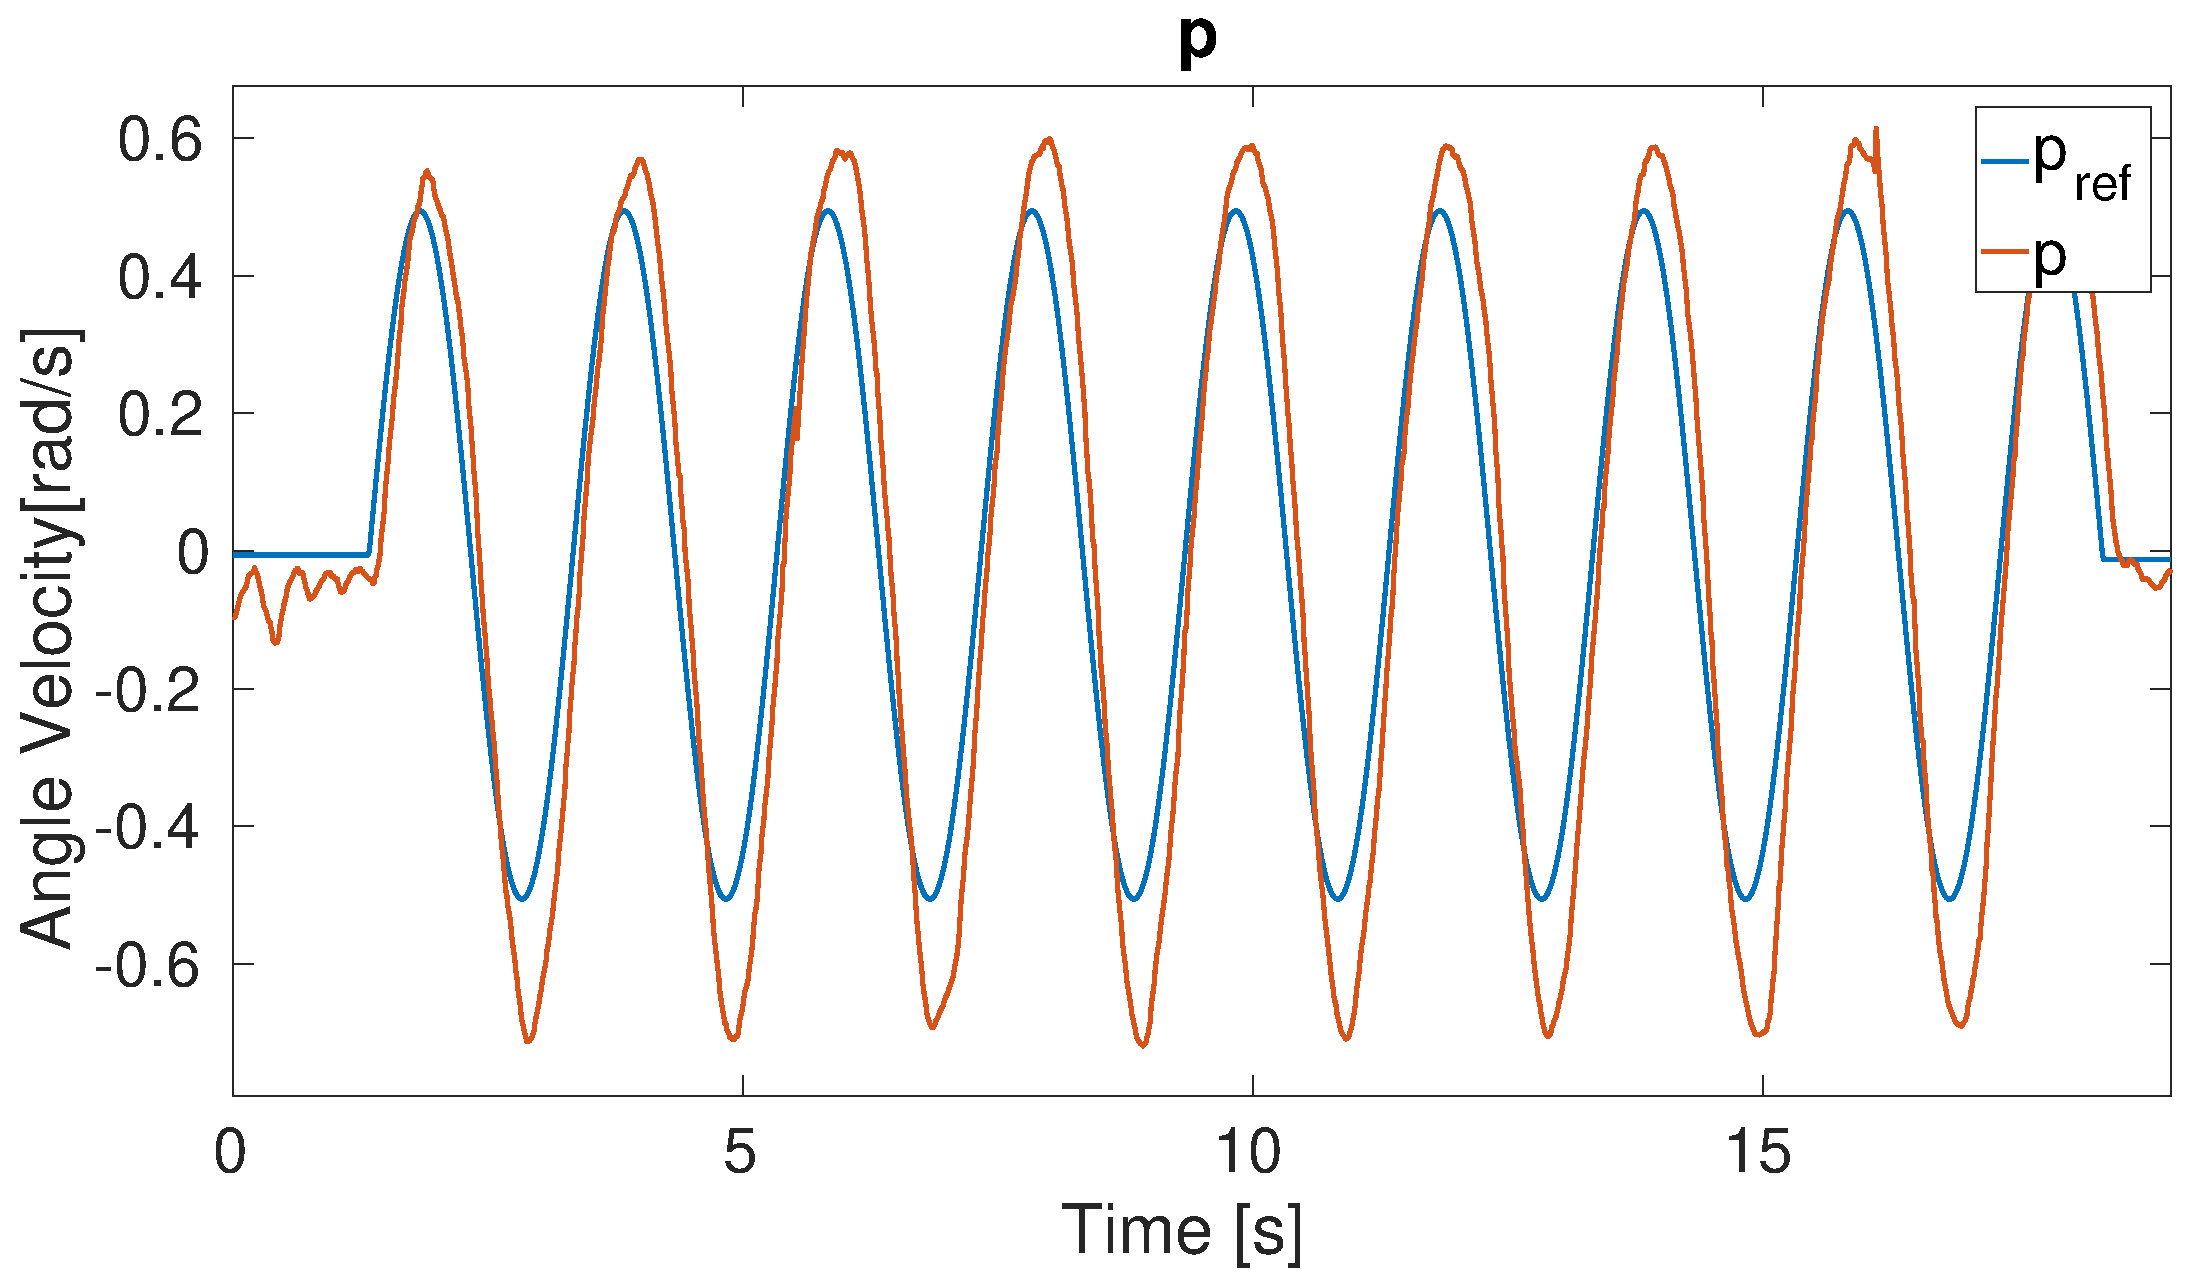
\includegraphics[width=0.4\textwidth]{testSinPA05}}
  \qquad
  \subfloat[][\label{fig:simSin05P} An step was applied to the simulated \abbrROV in $\rollVelocity$.]{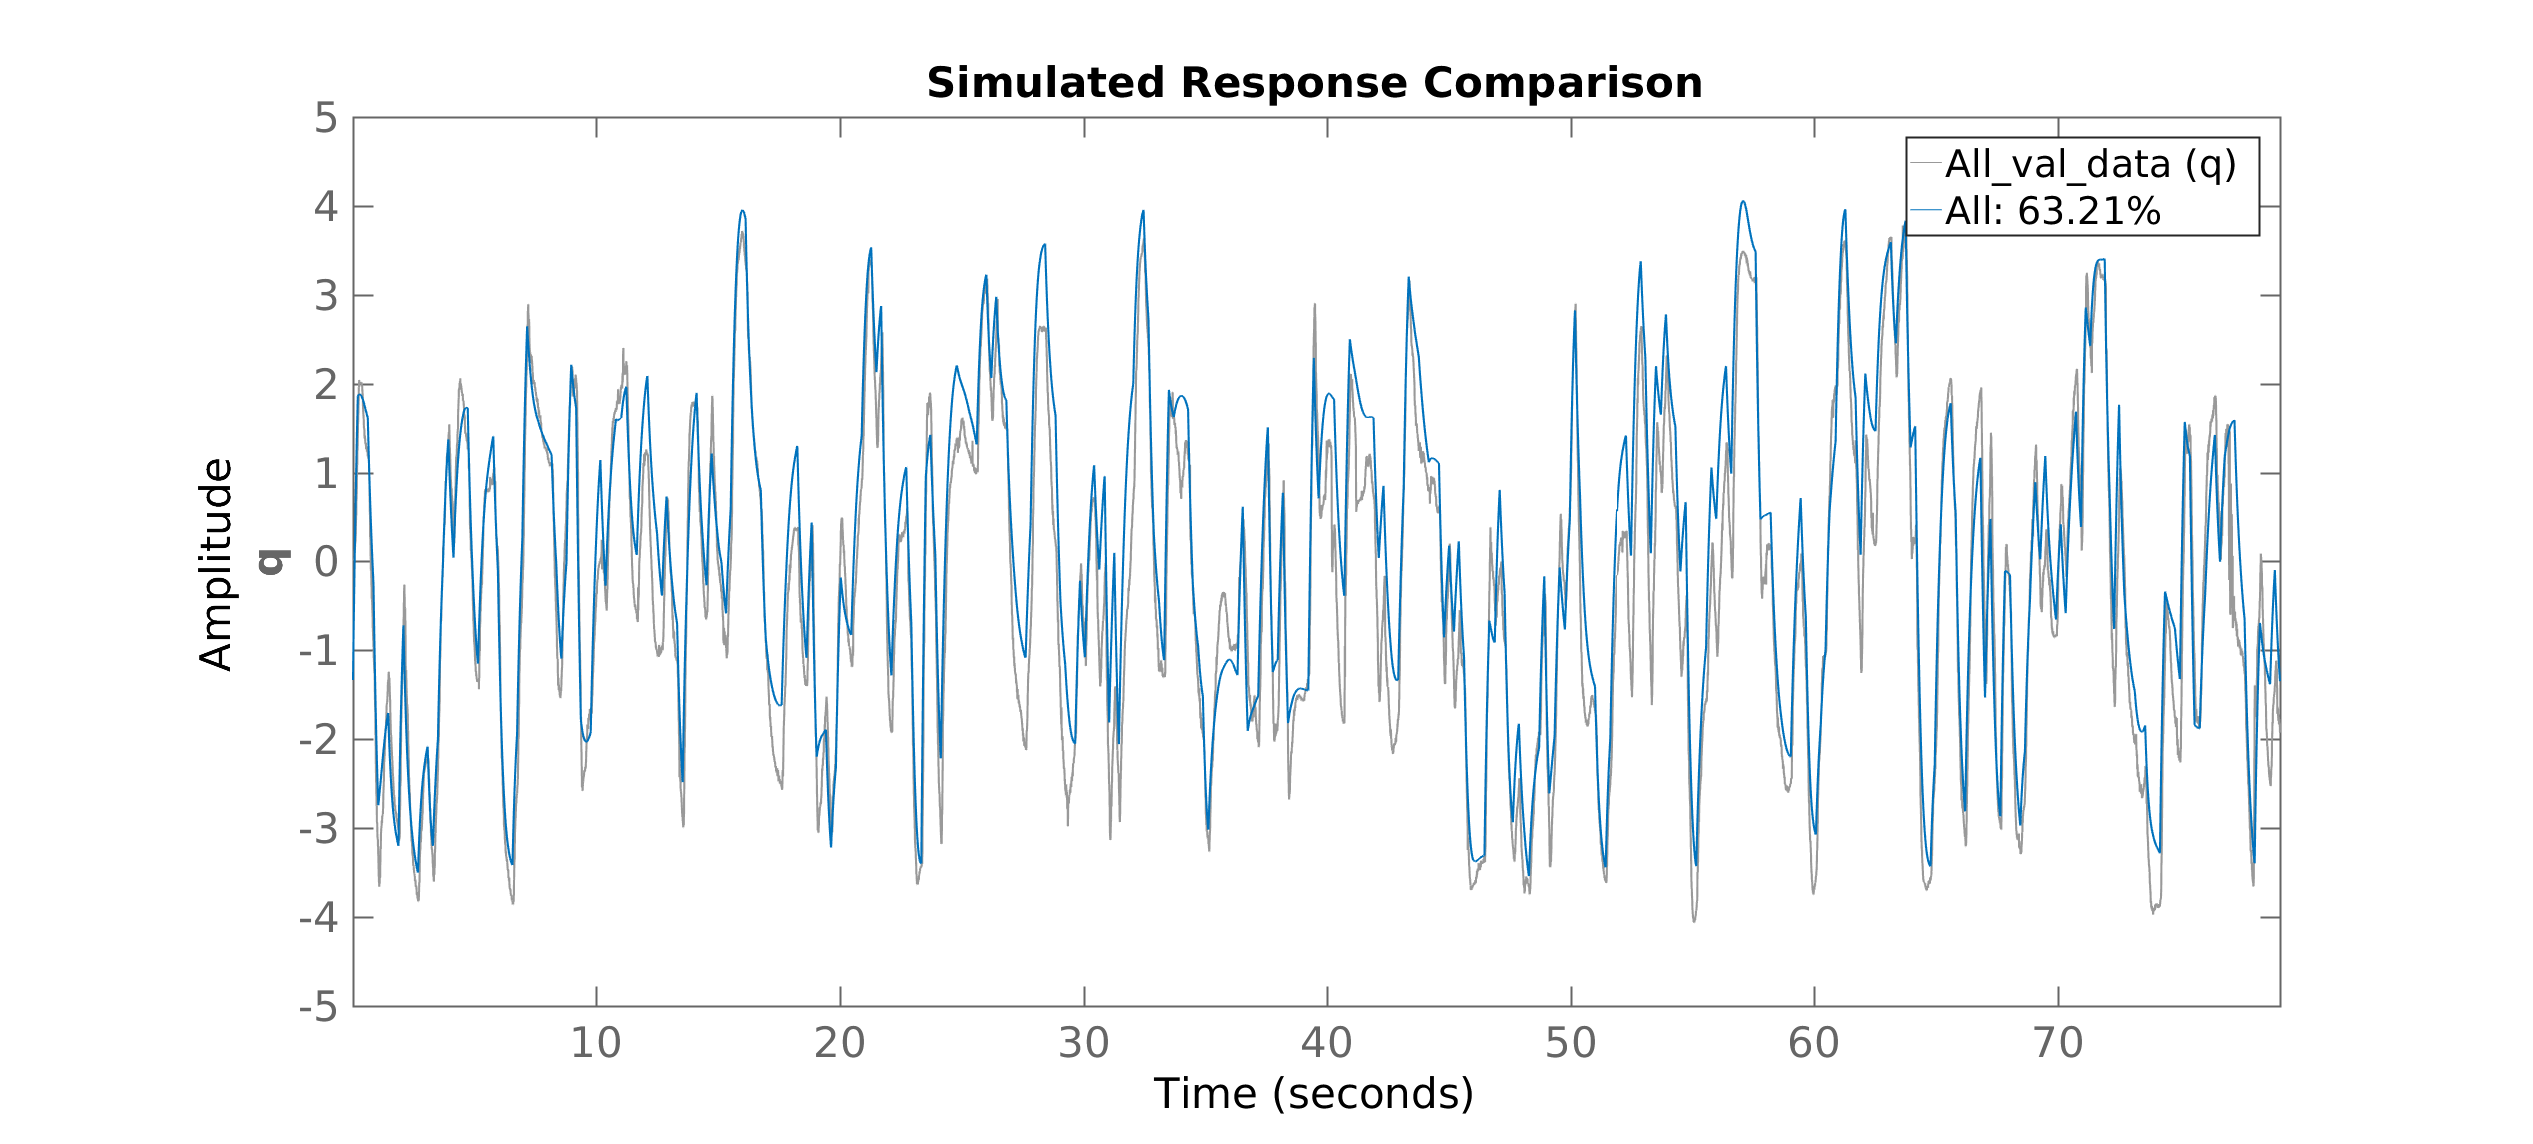
\includegraphics[width=0.4\textwidth]{velocityCompareq}}
  \qquad
  \subfloat[][\label{fig:testSin05Q} An step was applied to $\pitchVelocity$ .]{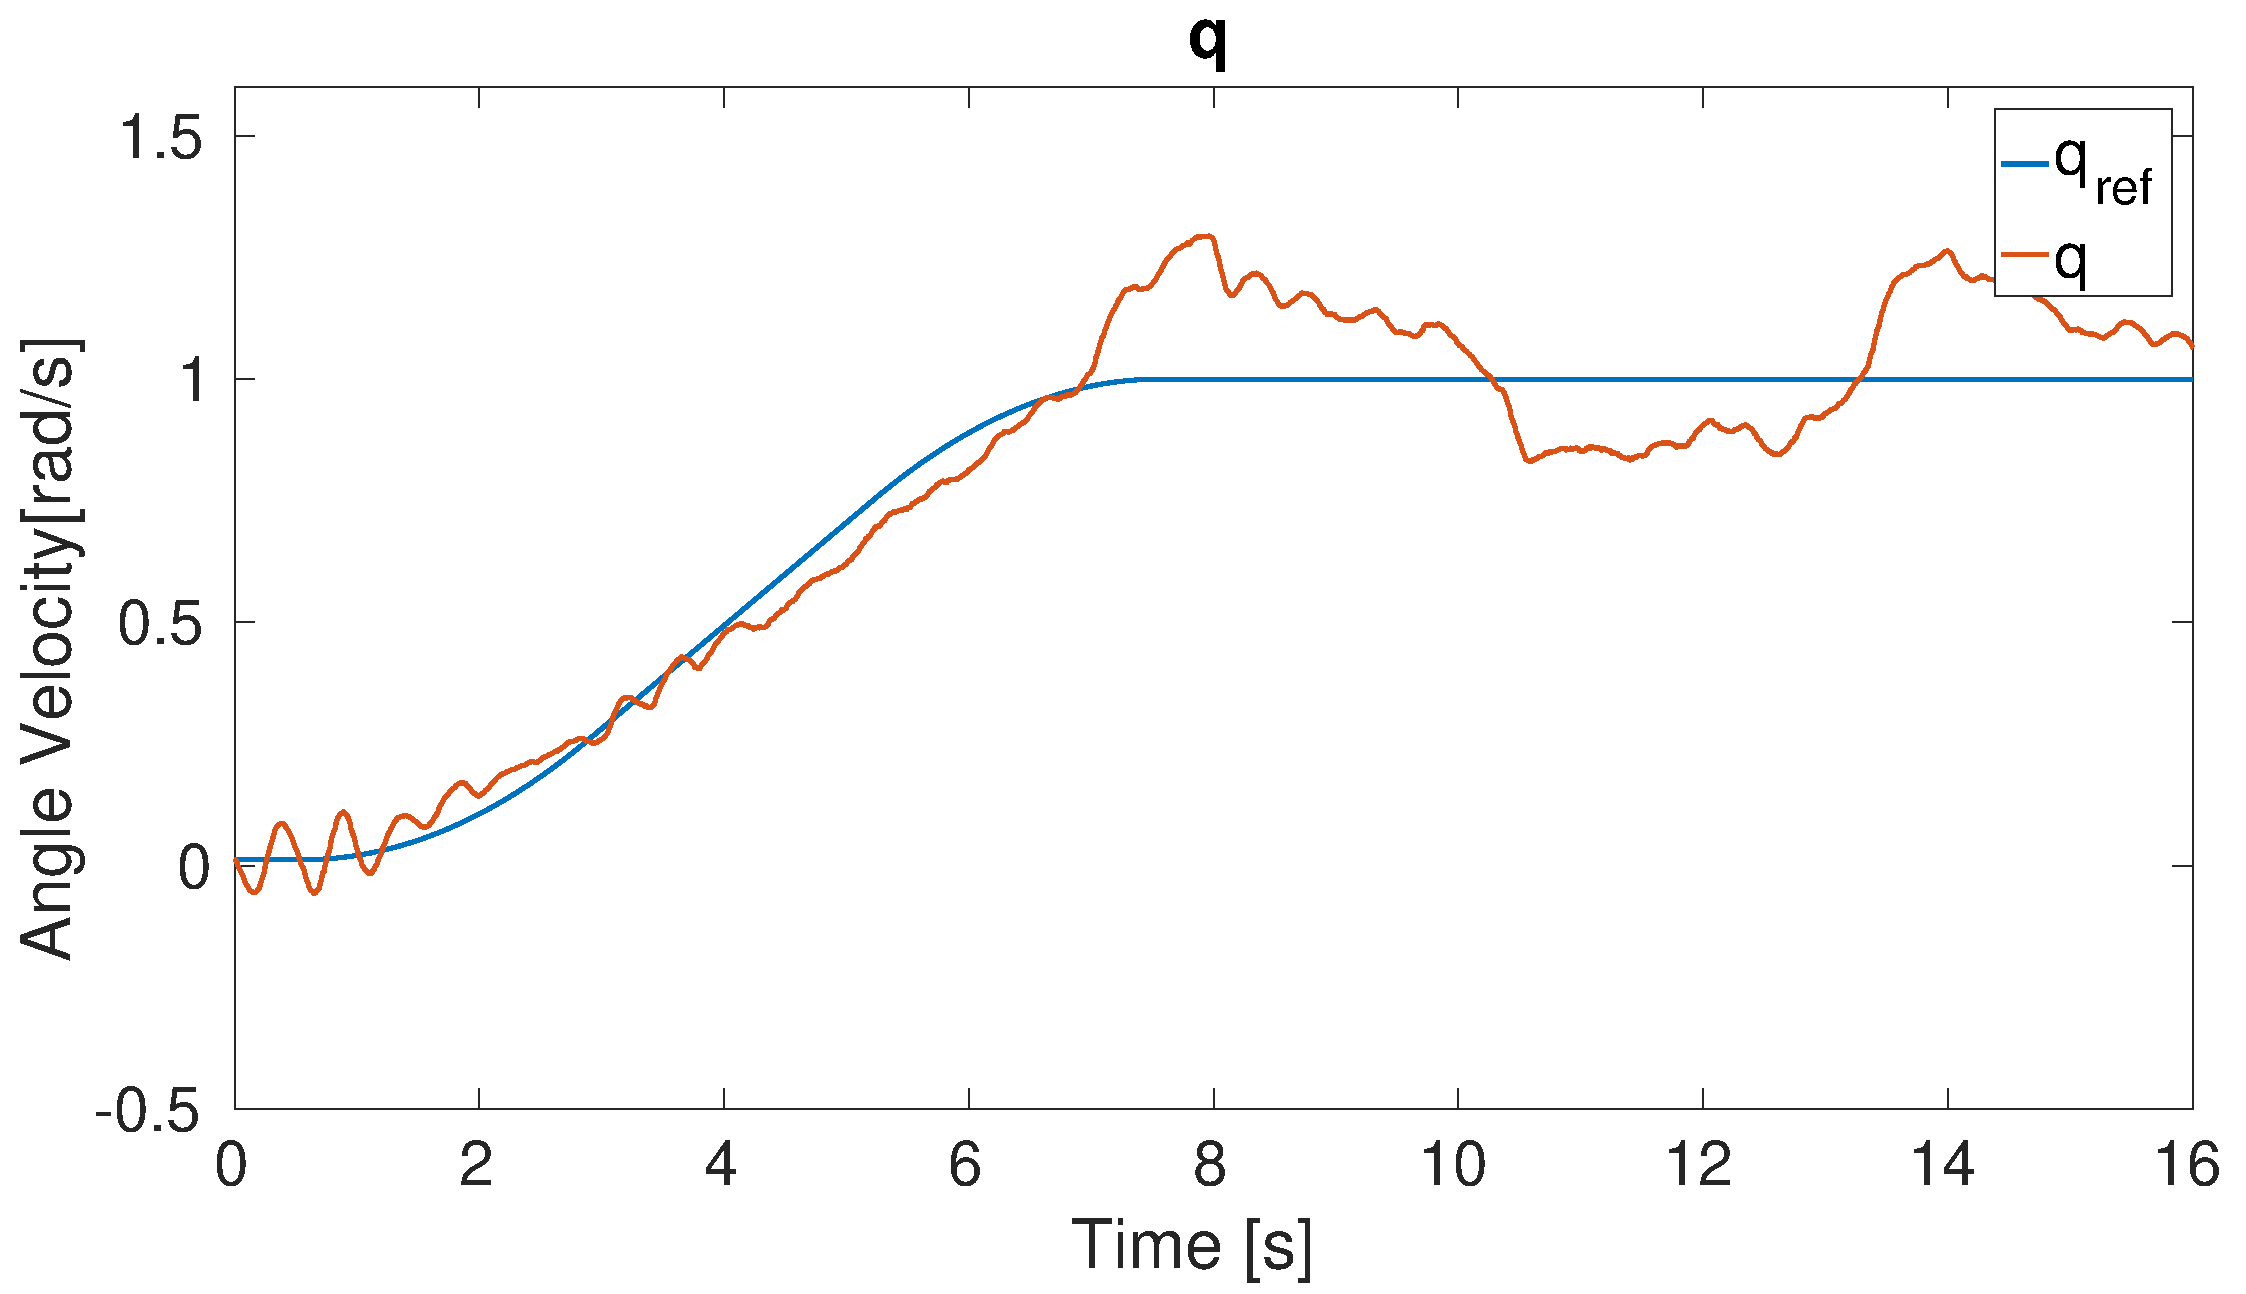
\includegraphics[width=0.4\textwidth]{testStepQs3e10a1}}
  \qquad
  \subfloat[][\label{fig:simSin05Q} An step was applied to the simulated \abbrROV in $\pitchVelocity$.]{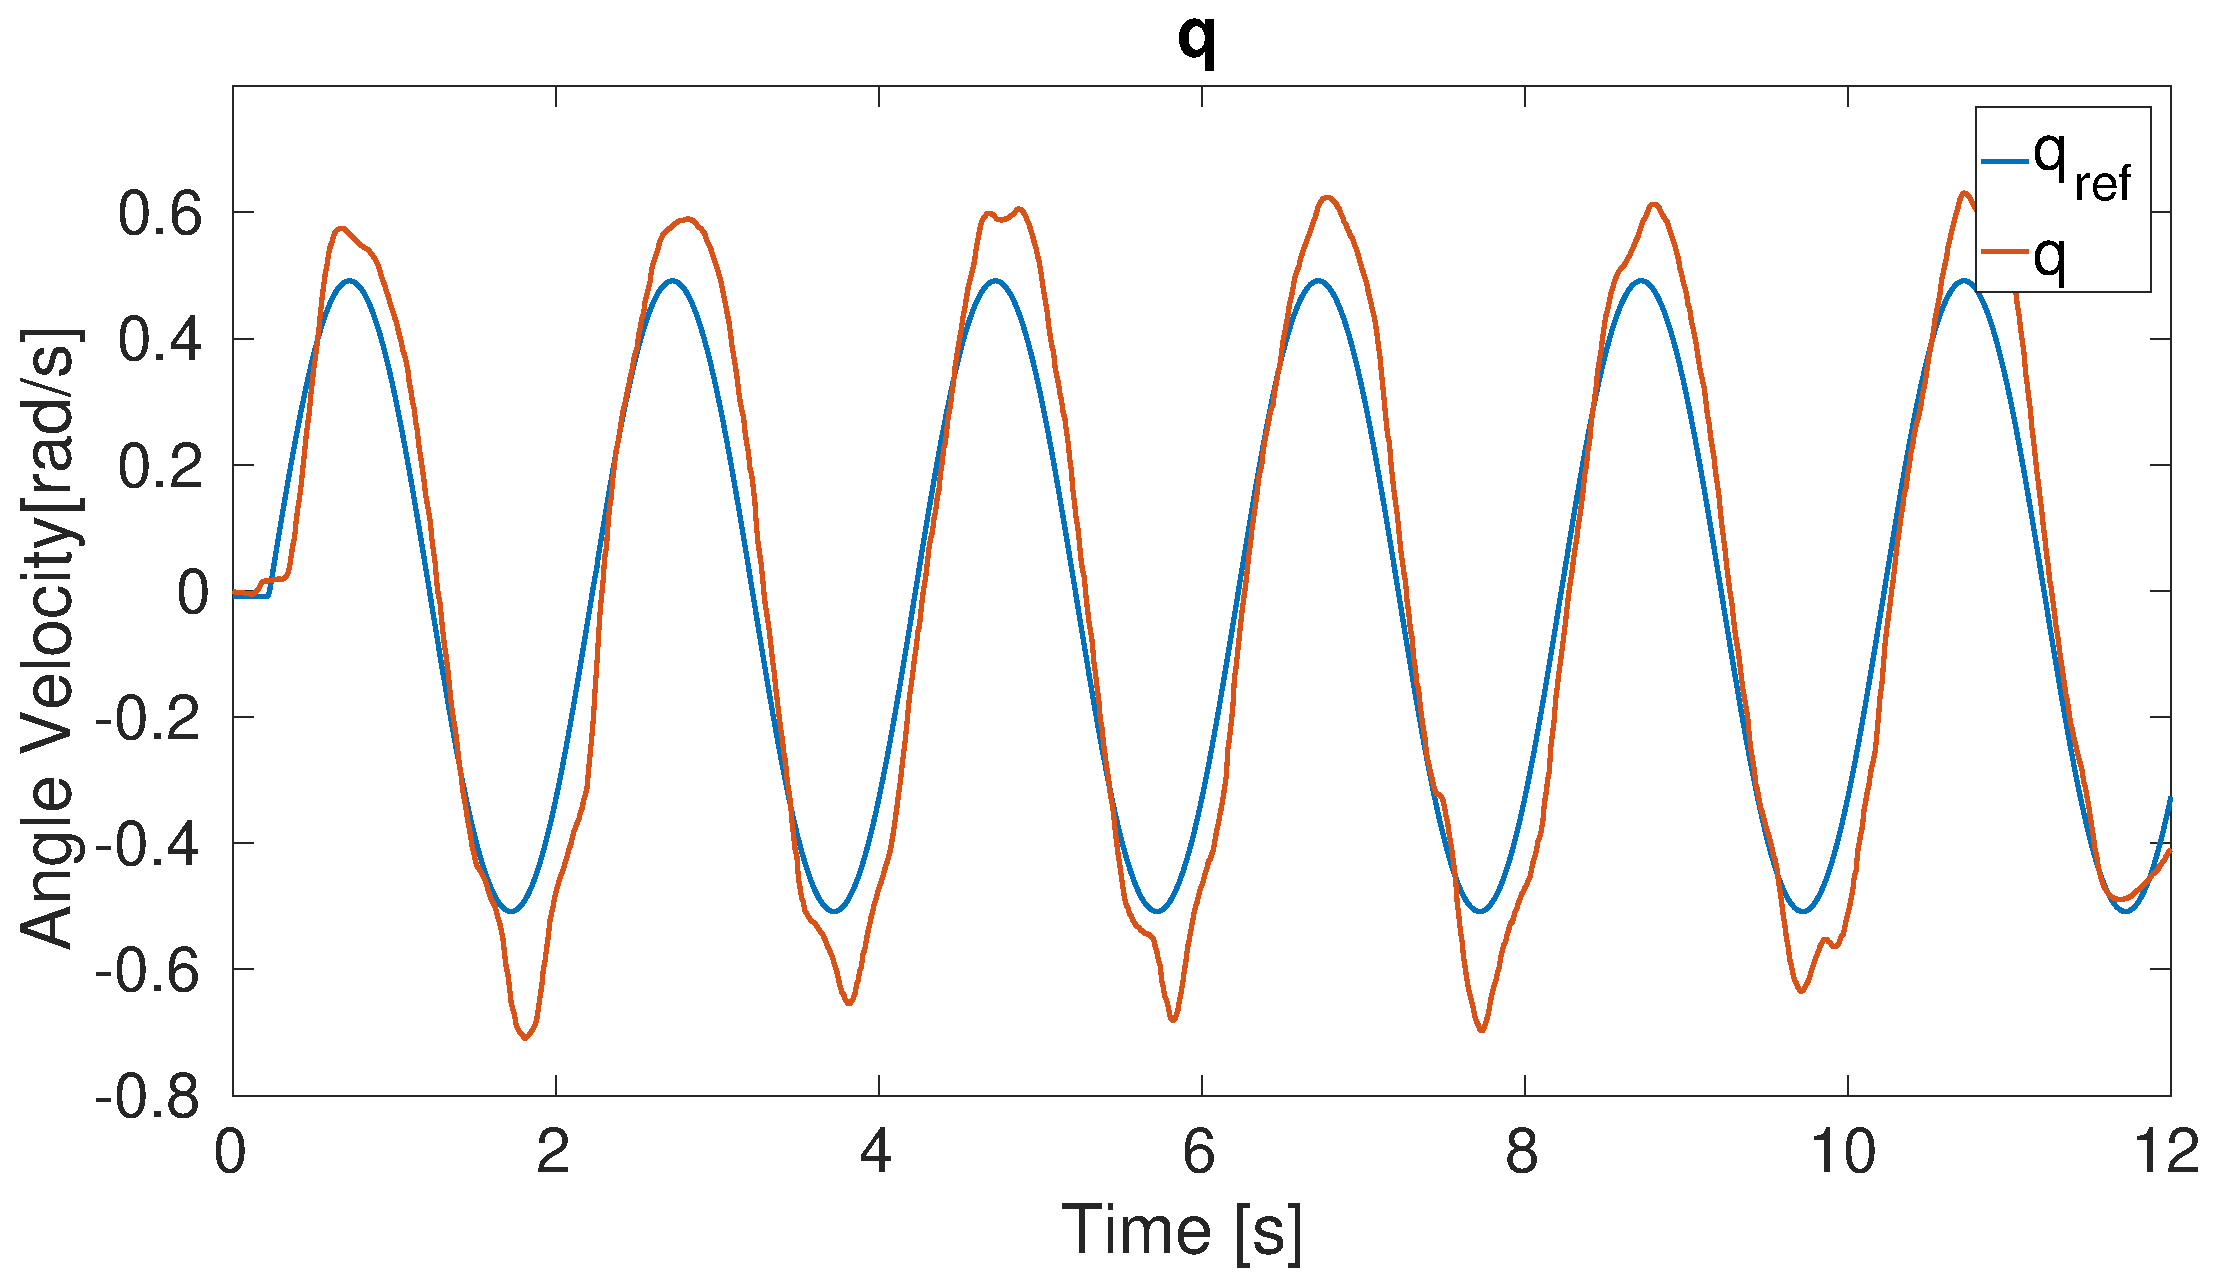
\includegraphics[width=0.4\textwidth]{testSinQA05}}
  \qquad
  \subfloat[][\label{fig:testSin05R} An step was applied to $\yawVelocity$ .]{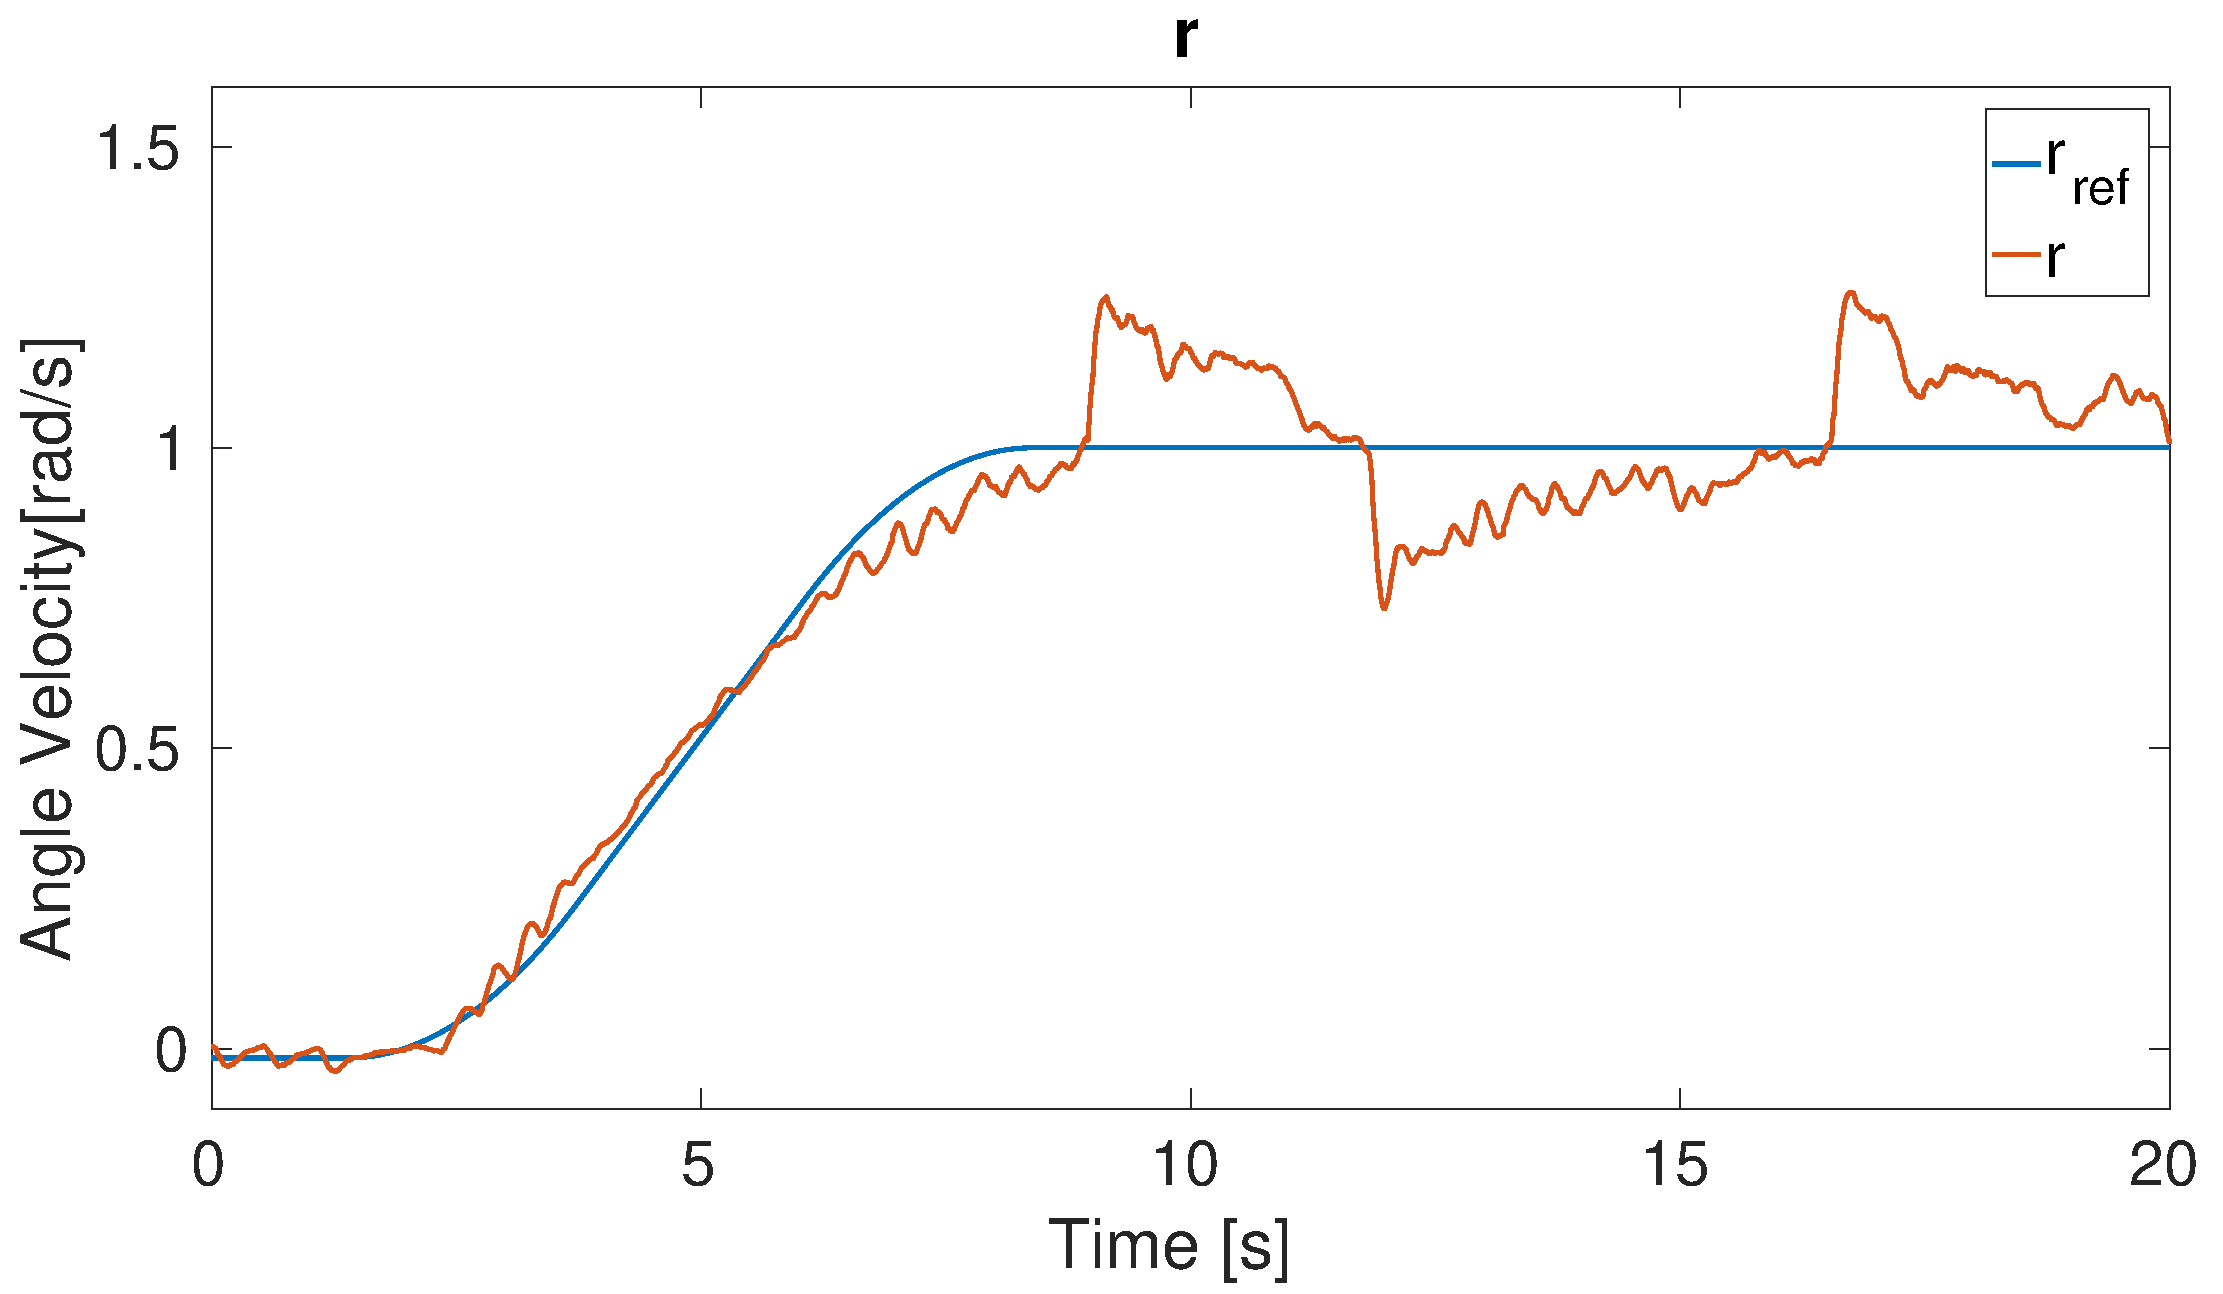
\includegraphics[width=0.4\textwidth]{testStepRs3e10a1}}
  \qquad
  \subfloat[][\label{fig:simSin50R} An step was applied to the simulated \abbrROV in $\yawVelocity$.]{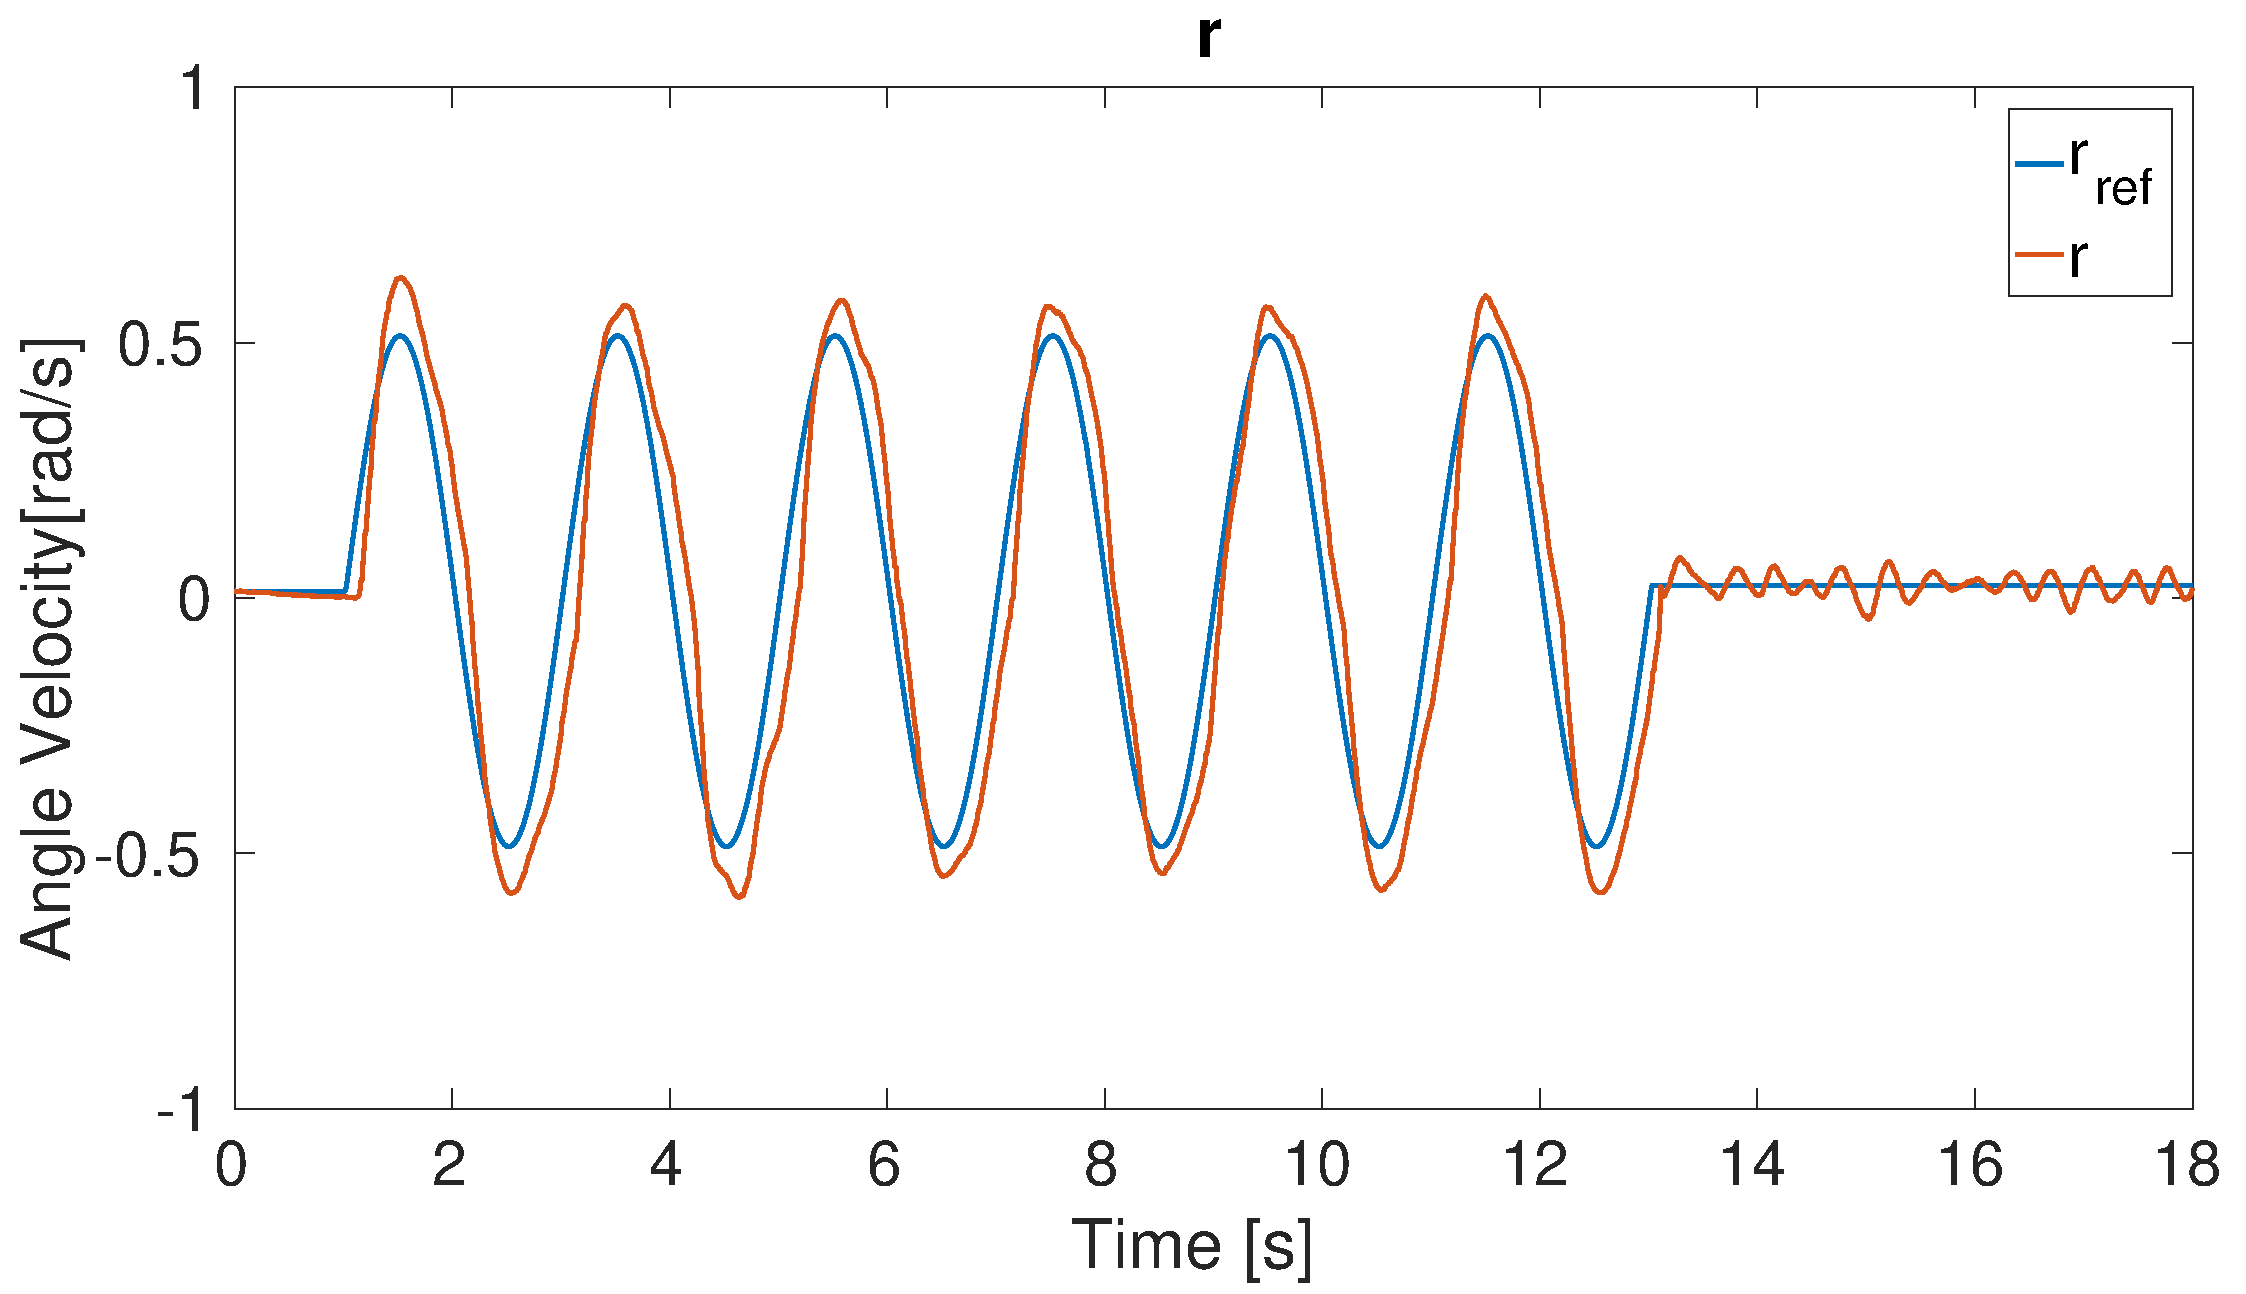
\includegraphics[width=0.4\textwidth]{testSinRA05}}
    \caption{\label{fig:Sin05Rate}%
    Comparison between simulation and a real test of a smooth step reference in.}
\end{figure}

\begin{figure}
\centering
  \subfloat[][\label{fig:testSinAll05PRate} An step was applied to all \abbrDOF.]{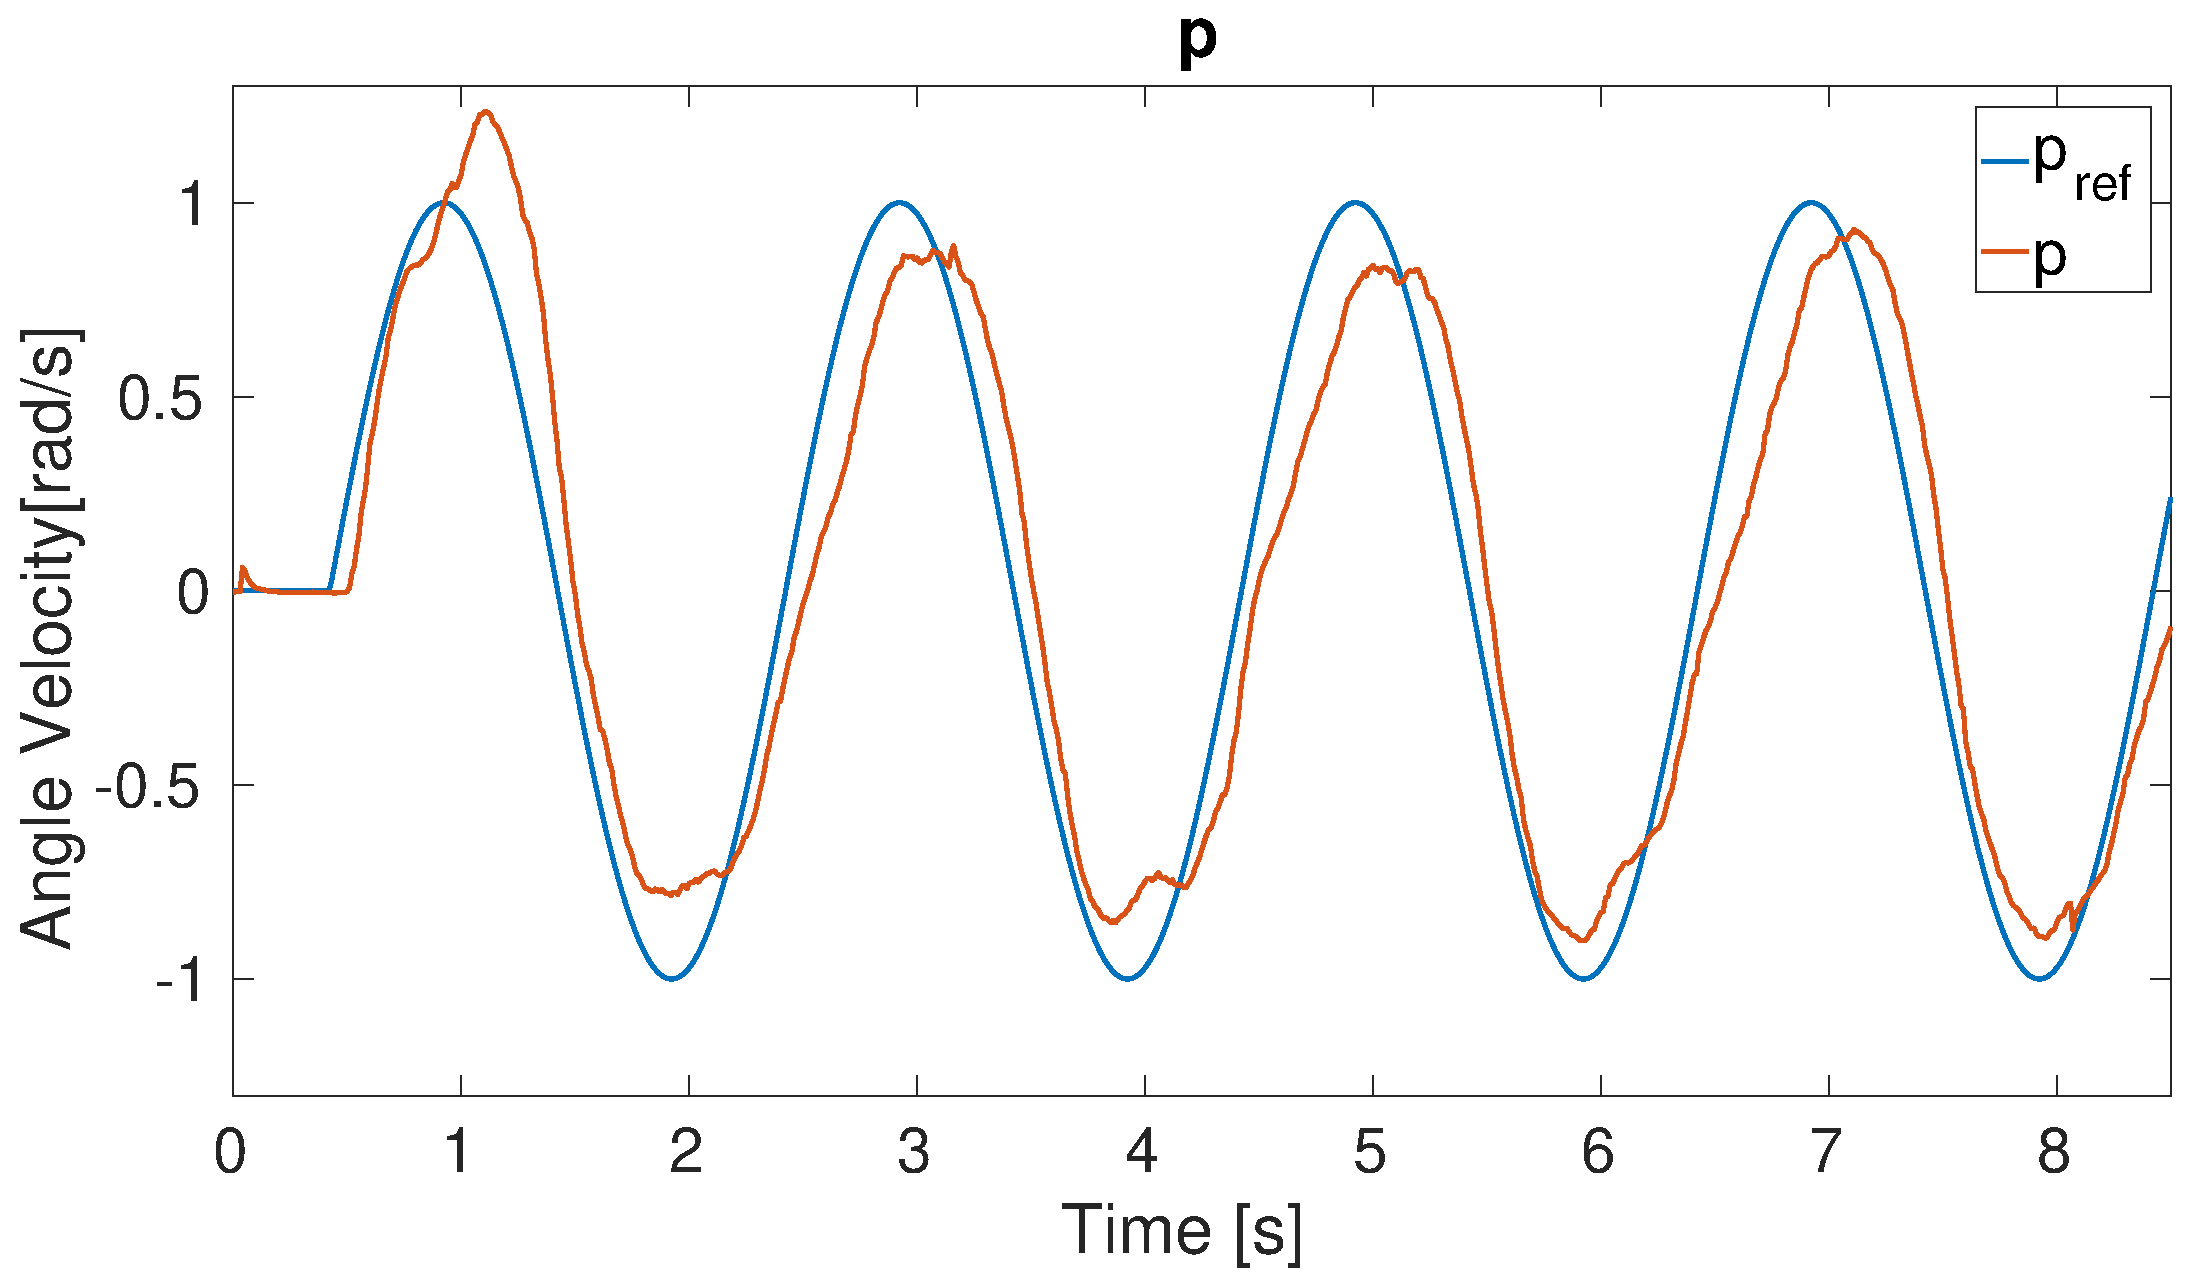
\includegraphics[width=0.4\textwidth]{testSinAllPA1}}
  \qquad
  \subfloat[][\label{fig:simSinAll05PRate} An step was applied to the simulated \abbrROV in all \abbrDOF.]{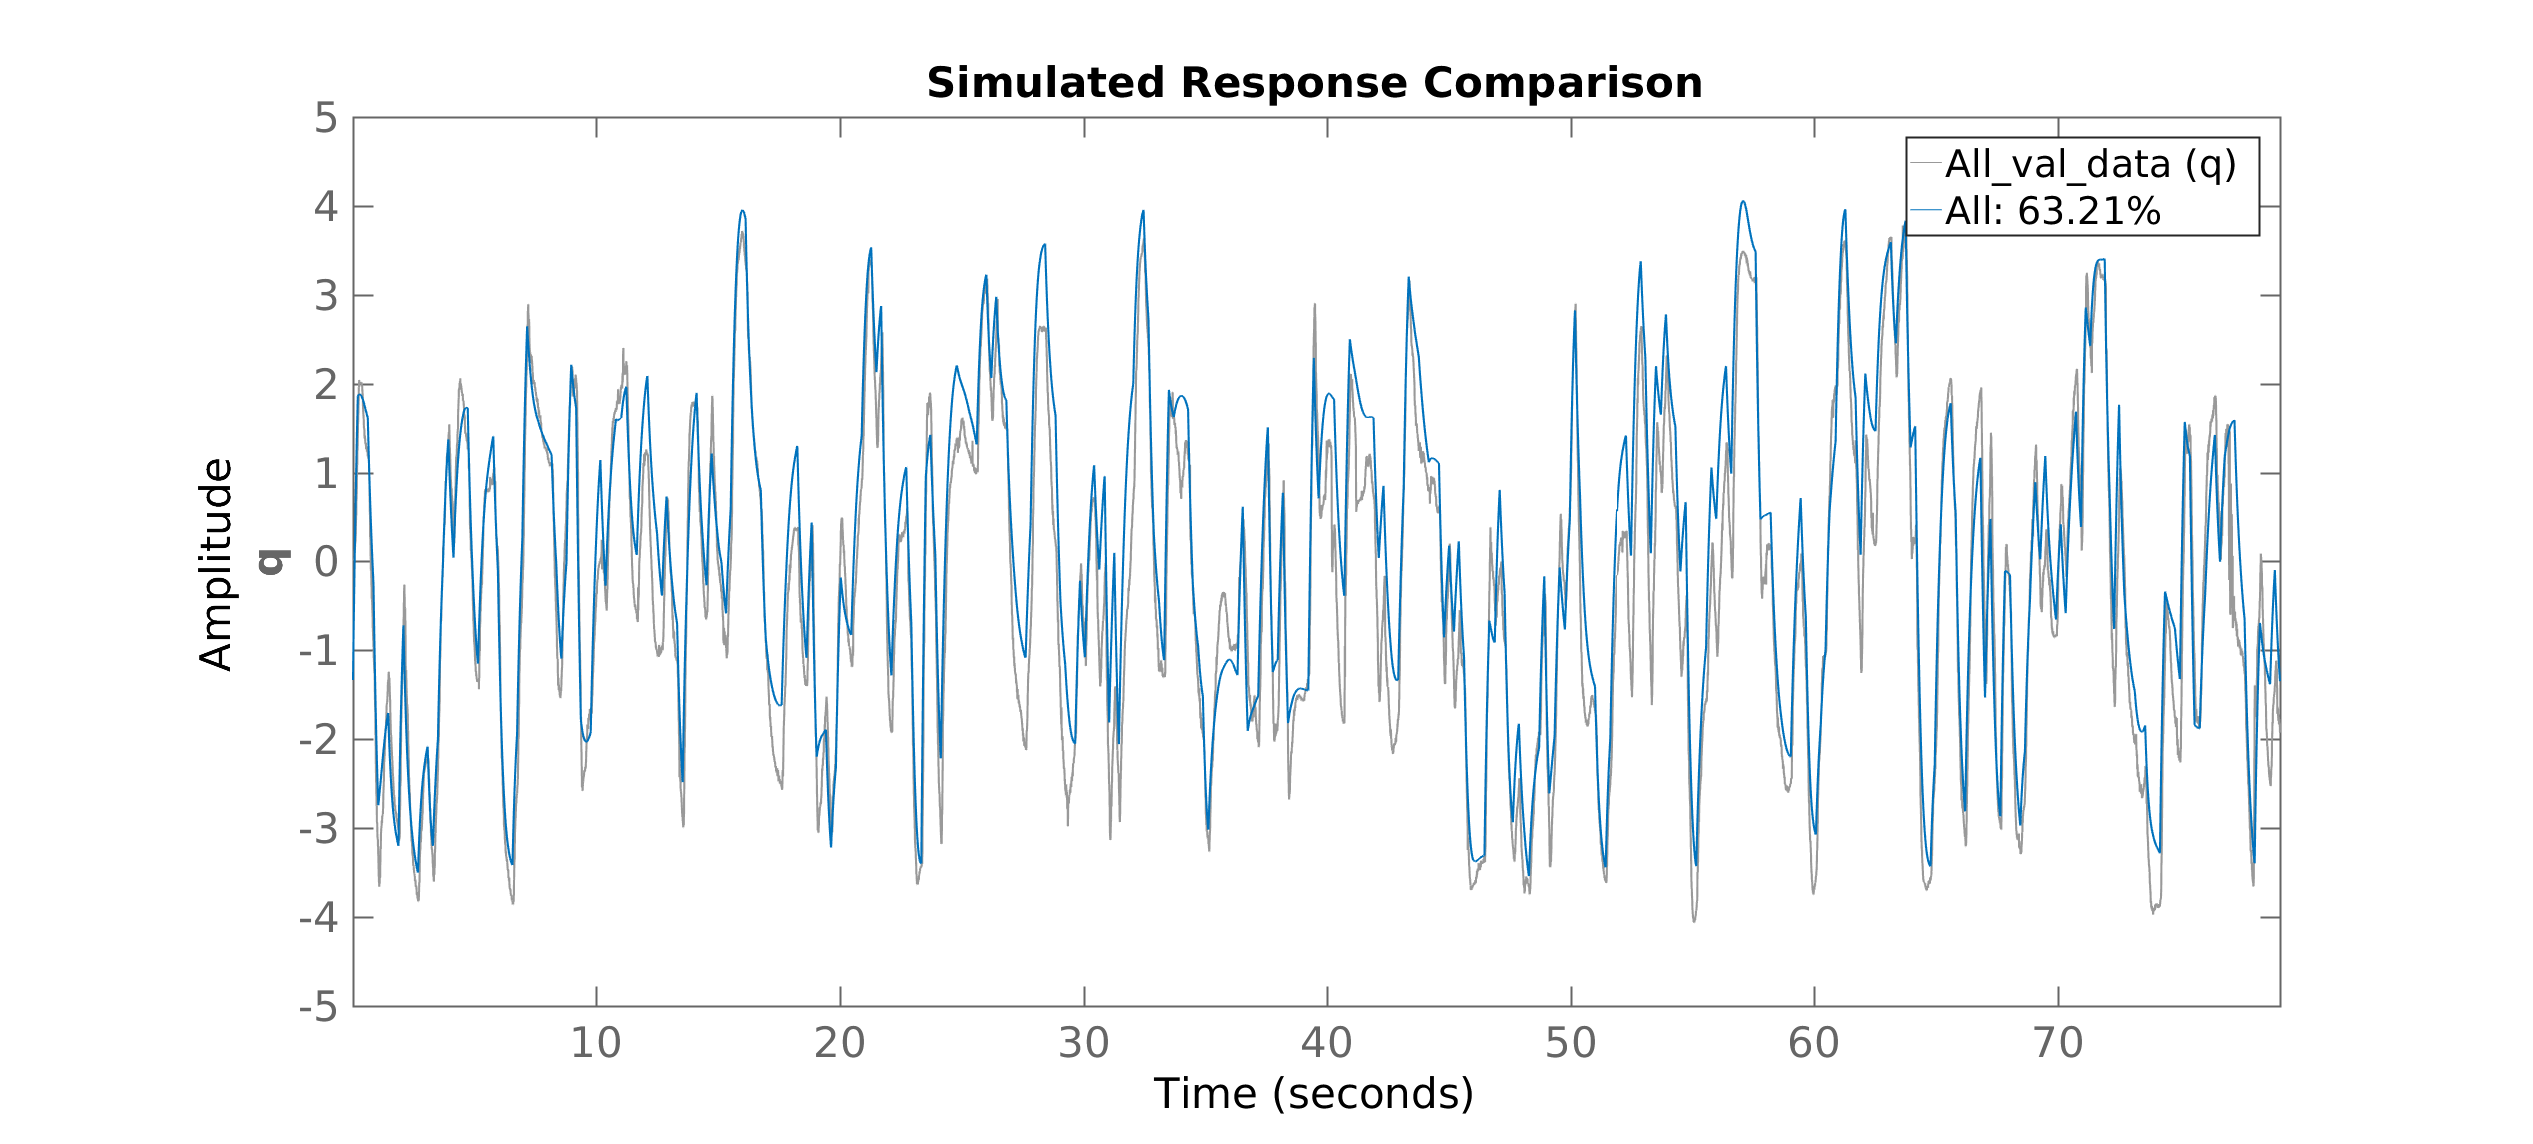
\includegraphics[width=0.4\textwidth]{velocityCompareq}}
  \qquad
  \subfloat[][\label{fig:TestSinAll05QRate} An step was applied to the simulated \abbrROV in all \abbrDOF.]{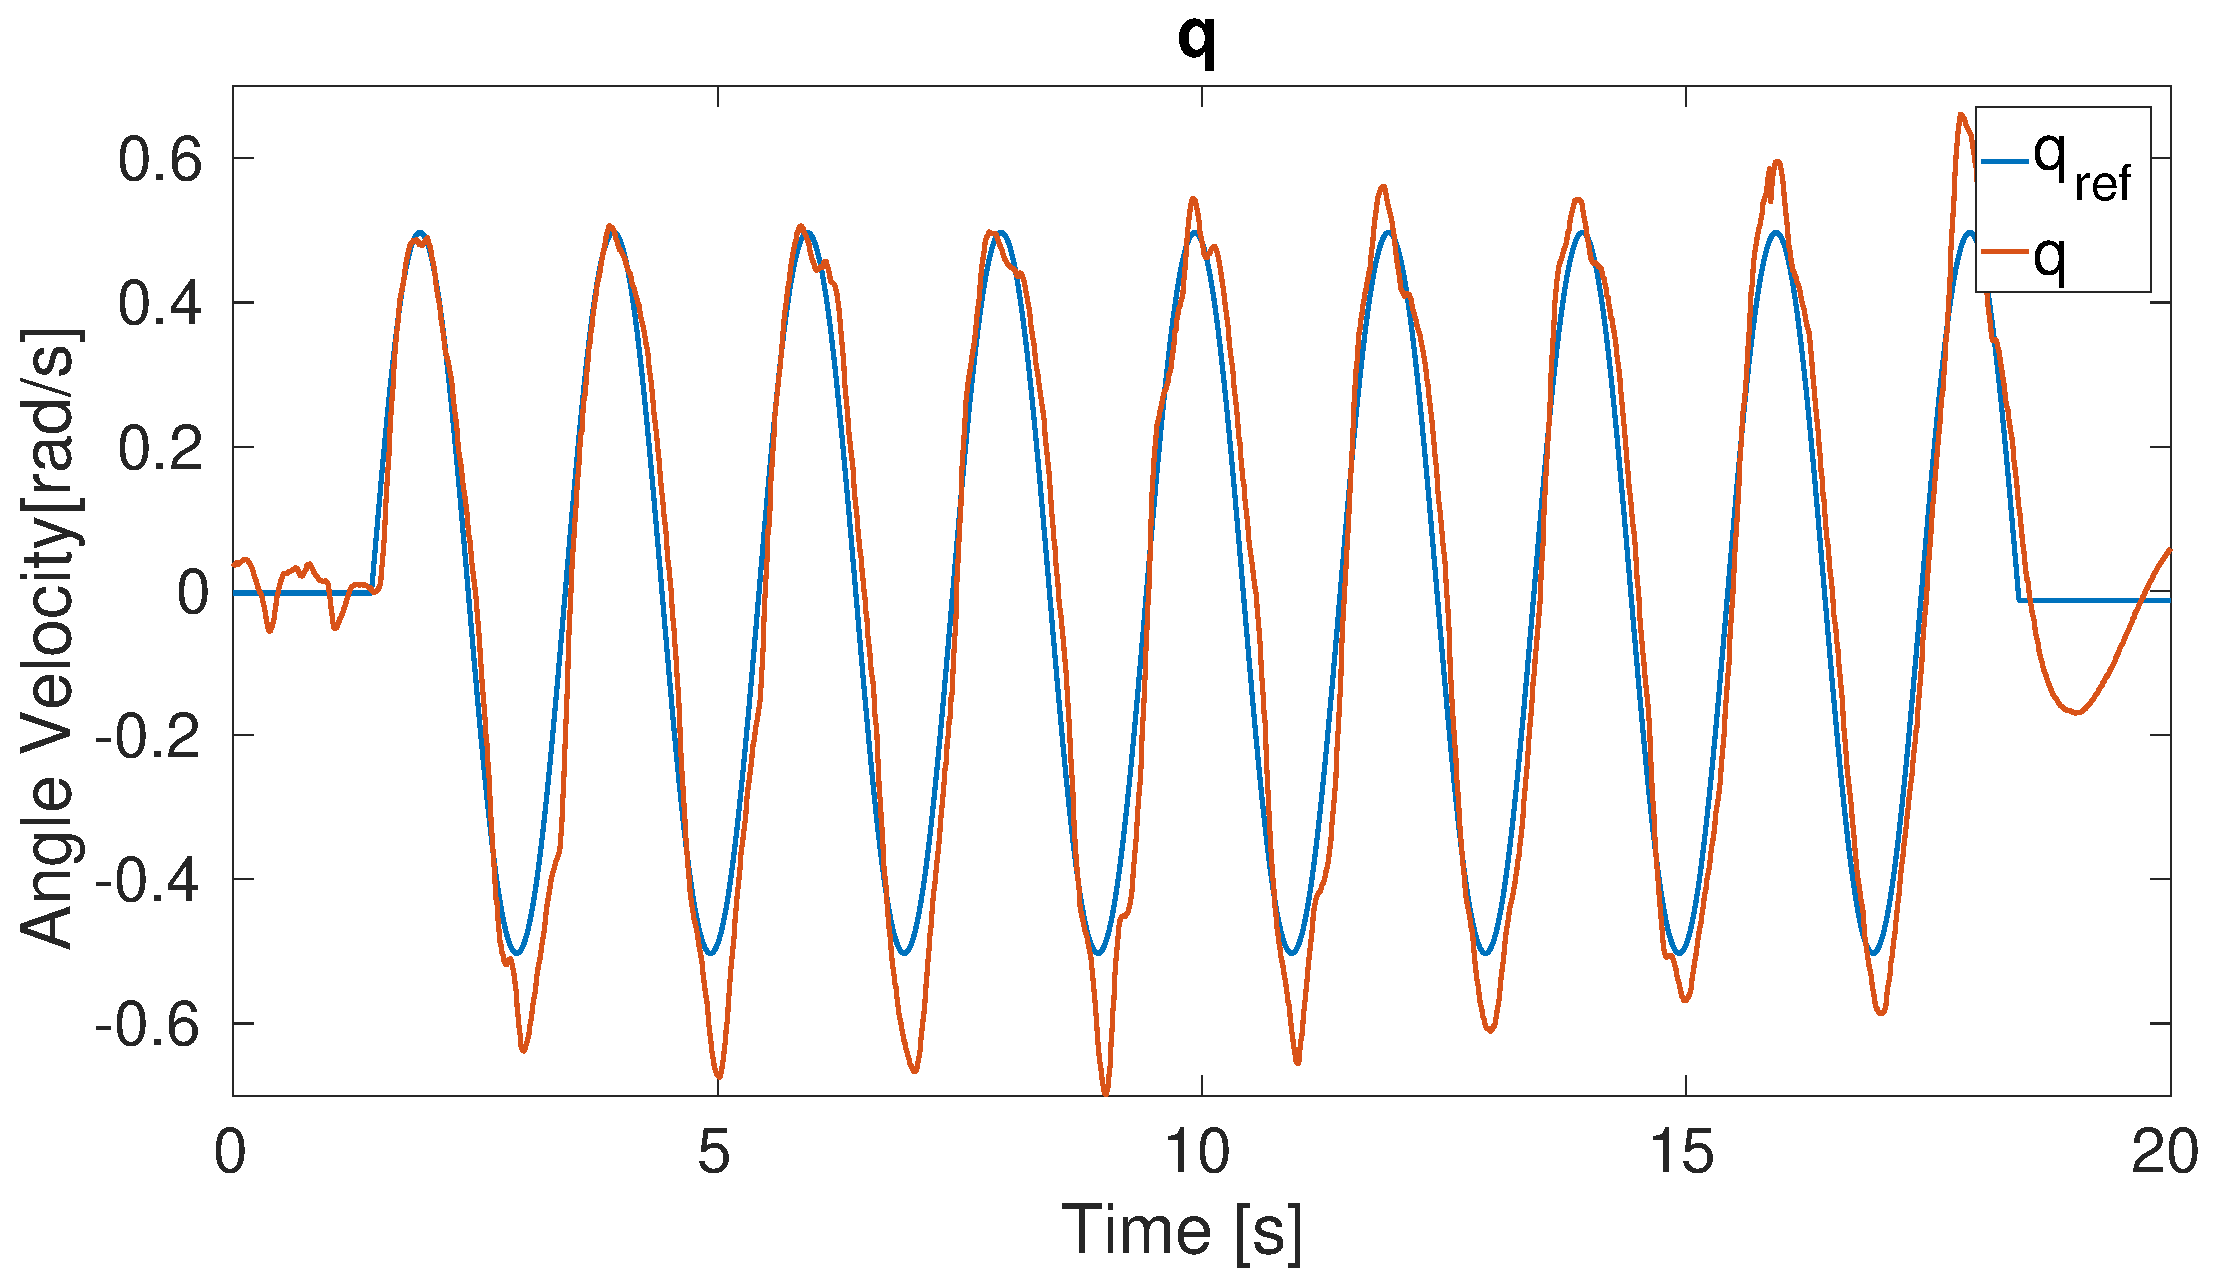
\includegraphics[width=0.4\textwidth]{testSinAllQA05}}
  \qquad
  \subfloat[][\label{fig:simSinAll05QRate} An step was applied to the simulated \abbrROV in all \abbrDOF.]{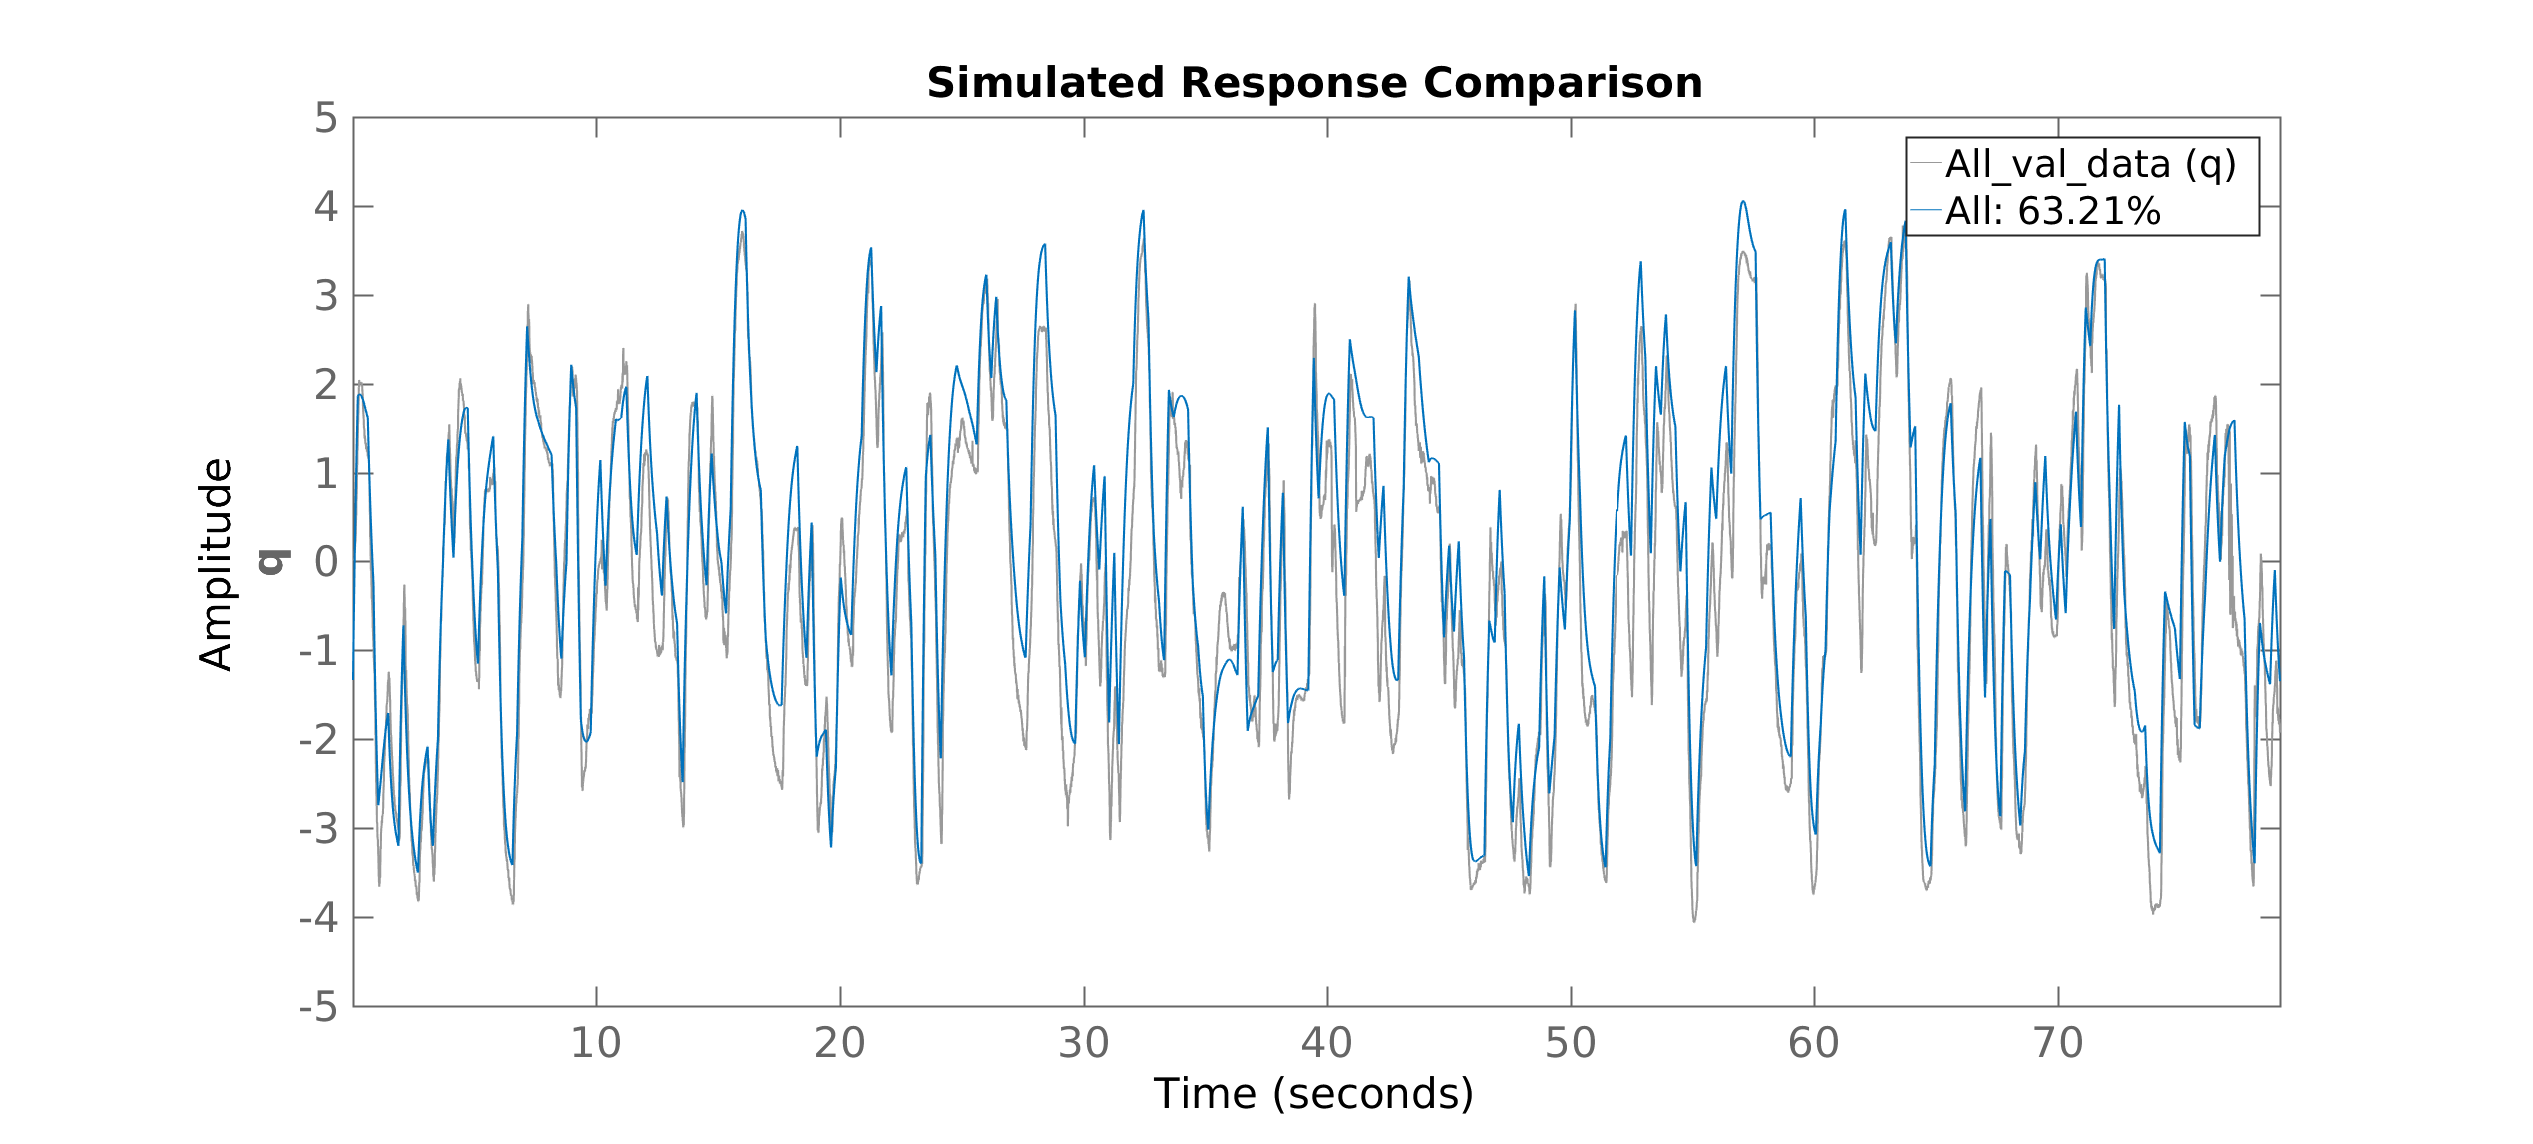
\includegraphics[width=0.4\textwidth]{velocityCompareq}}
  \qquad
  \subfloat[][\label{fig:TestSinAll05RRate} An step was applied to the simulated \abbrROV in all \abbrDOF.]{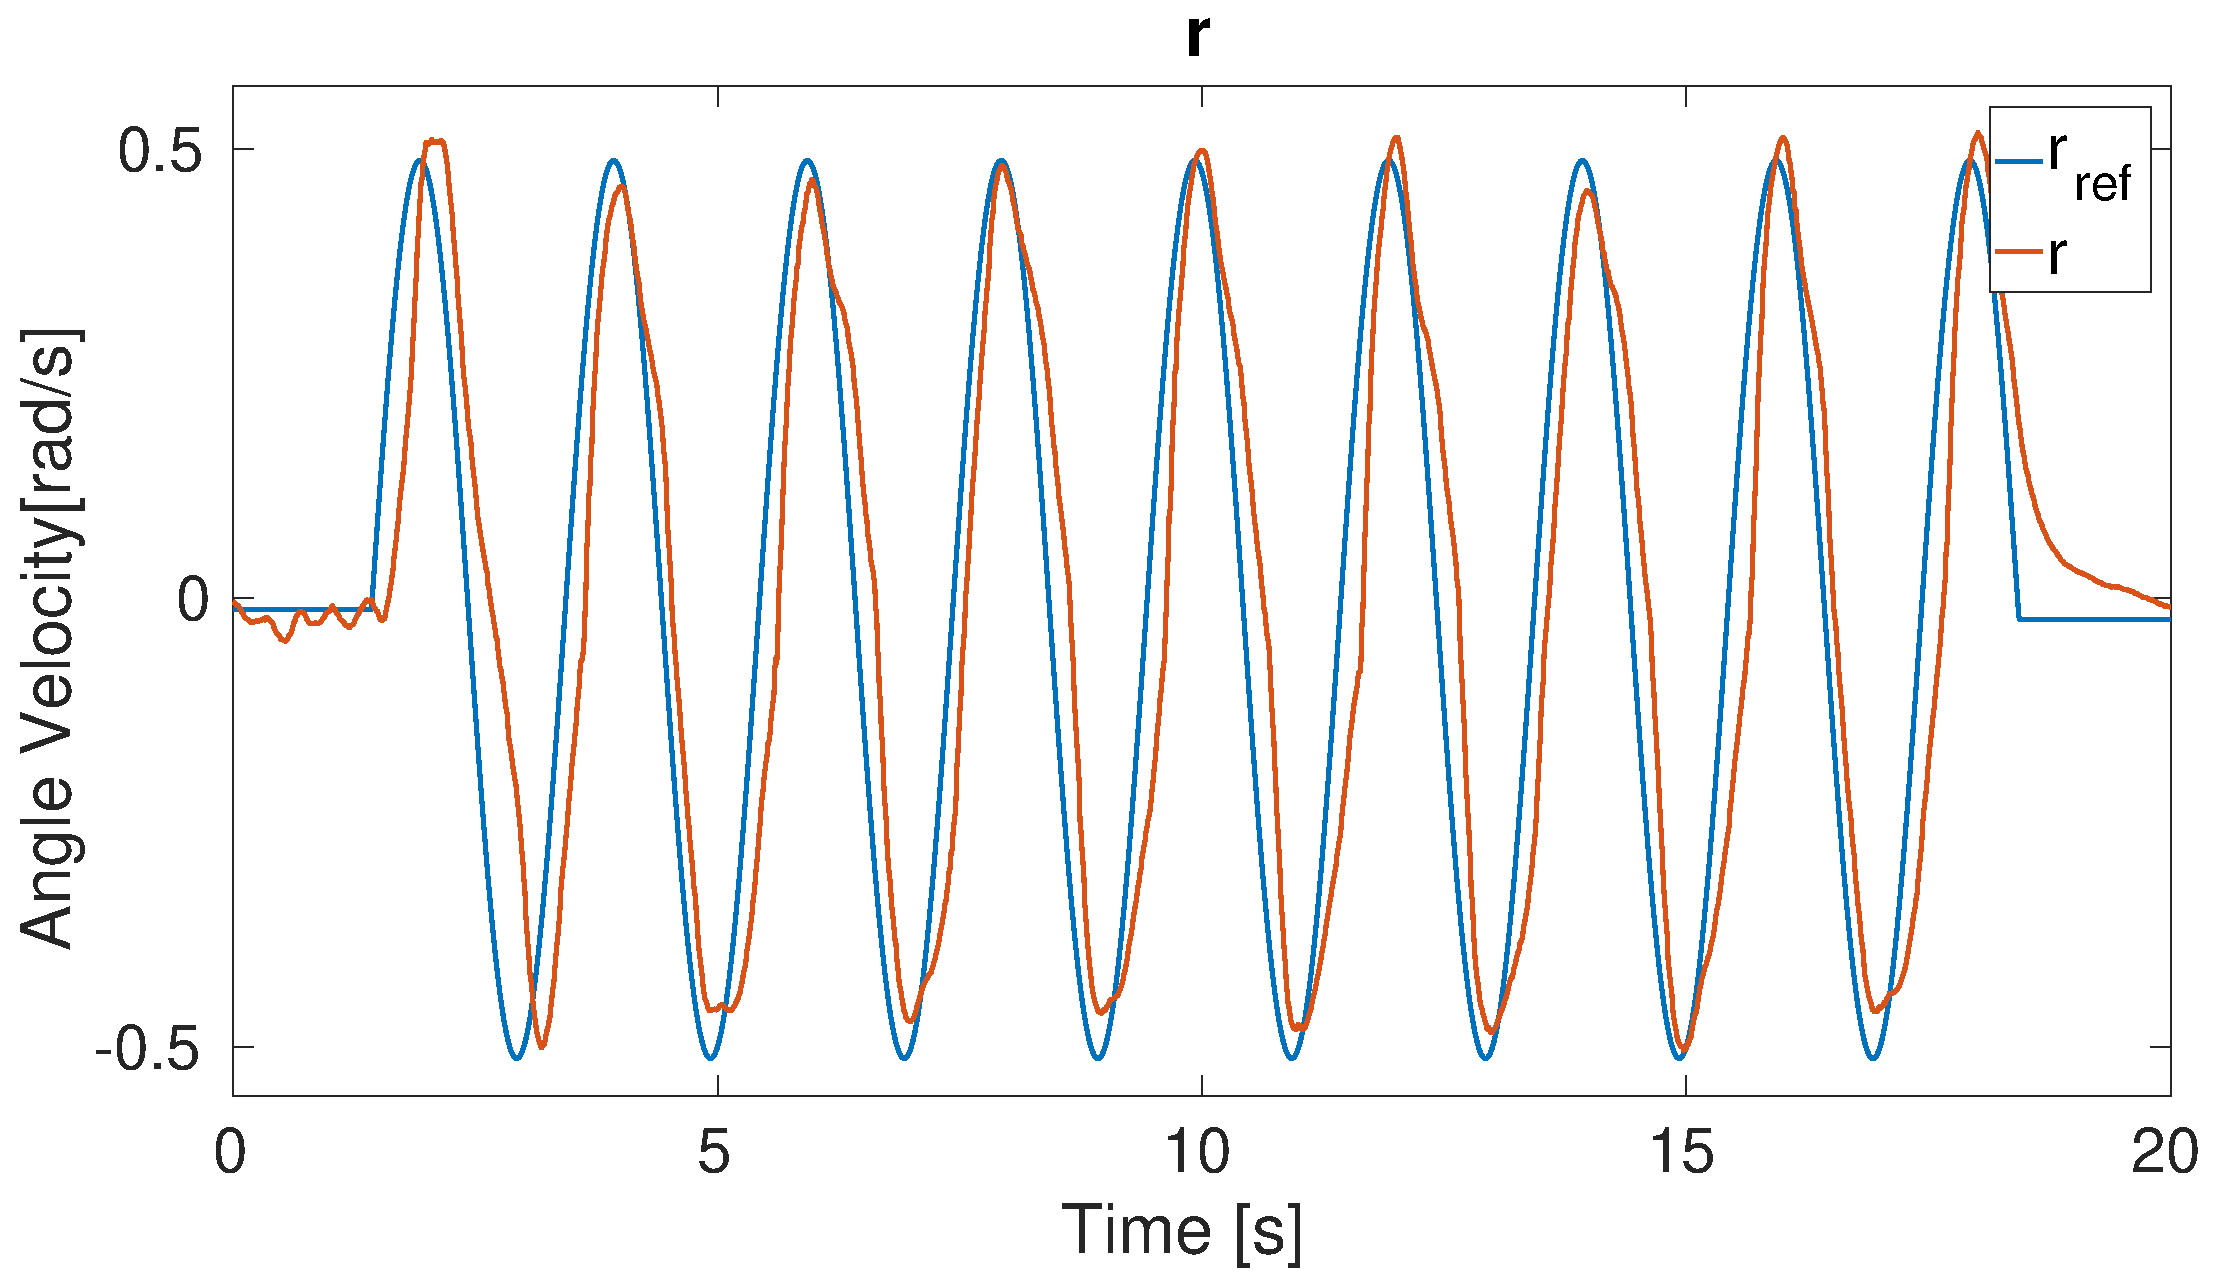
\includegraphics[width=0.4\textwidth]{testSinAllRA05}}
  \qquad
  \subfloat[][\label{fig:simSinAll05RRate} An step was applied to the simulated \abbrROV in all \abbrDOF.]{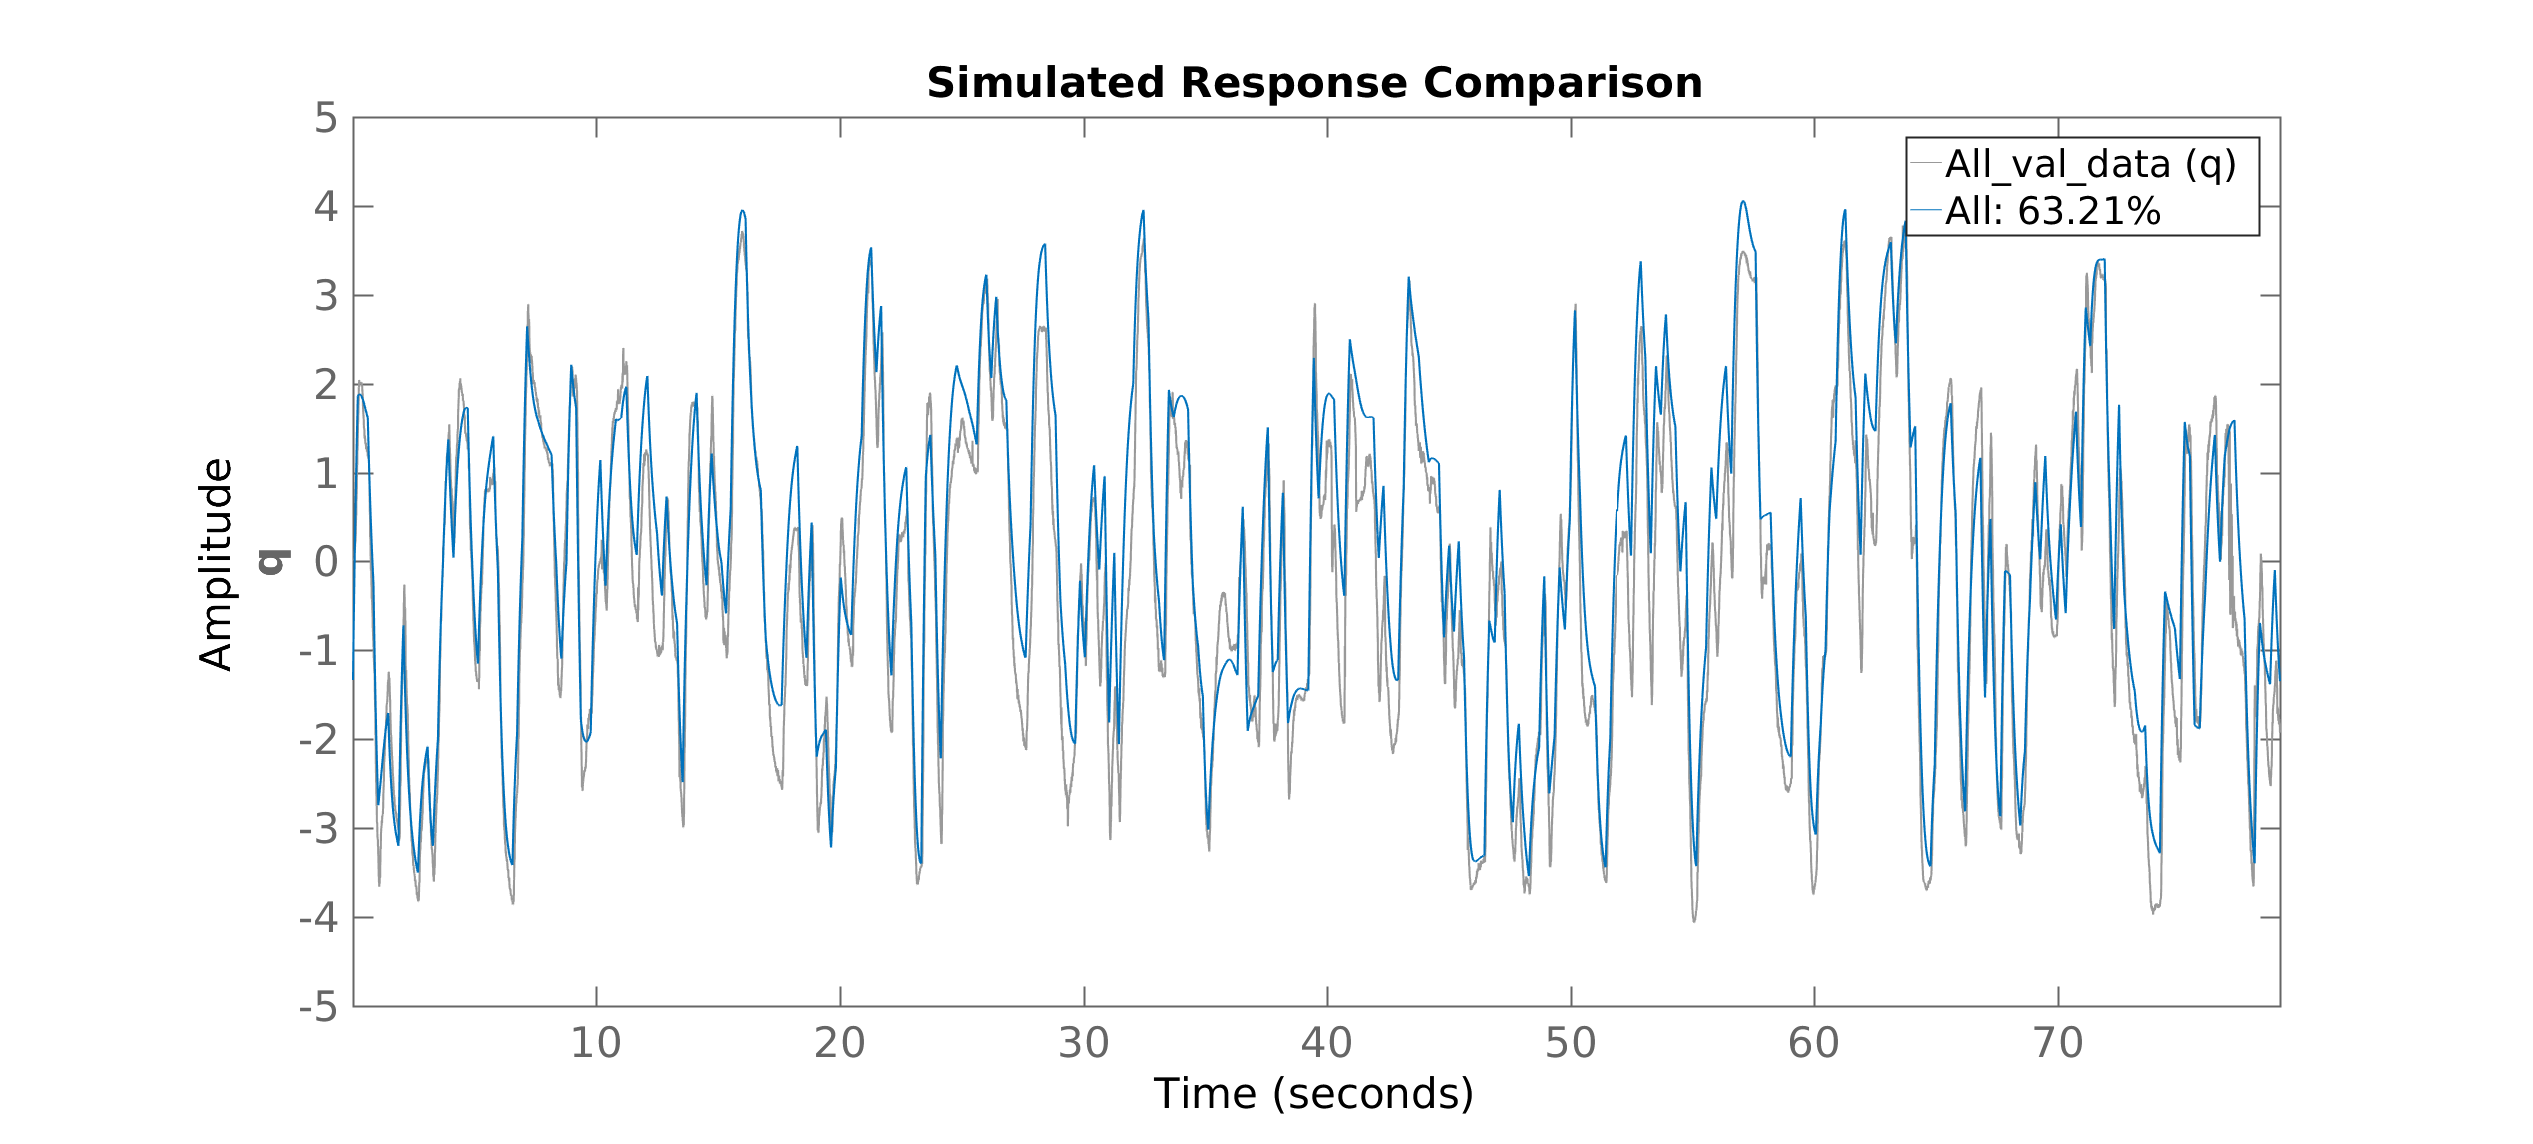
\includegraphics[width=0.4\textwidth]{velocityCompareq}}
  \caption{\label{fig:Sin1All05Rate}%
  }
\end{figure}

%%%%%%%%%%%%%%%%%%%%%%%%%%%Depth%%%%%%%%%%%%%%%%
\begin{figure}[tbp]
  \centering
  \subfloat[][\label{fig:testStepD1} An step was applied to $\zPosition$.]{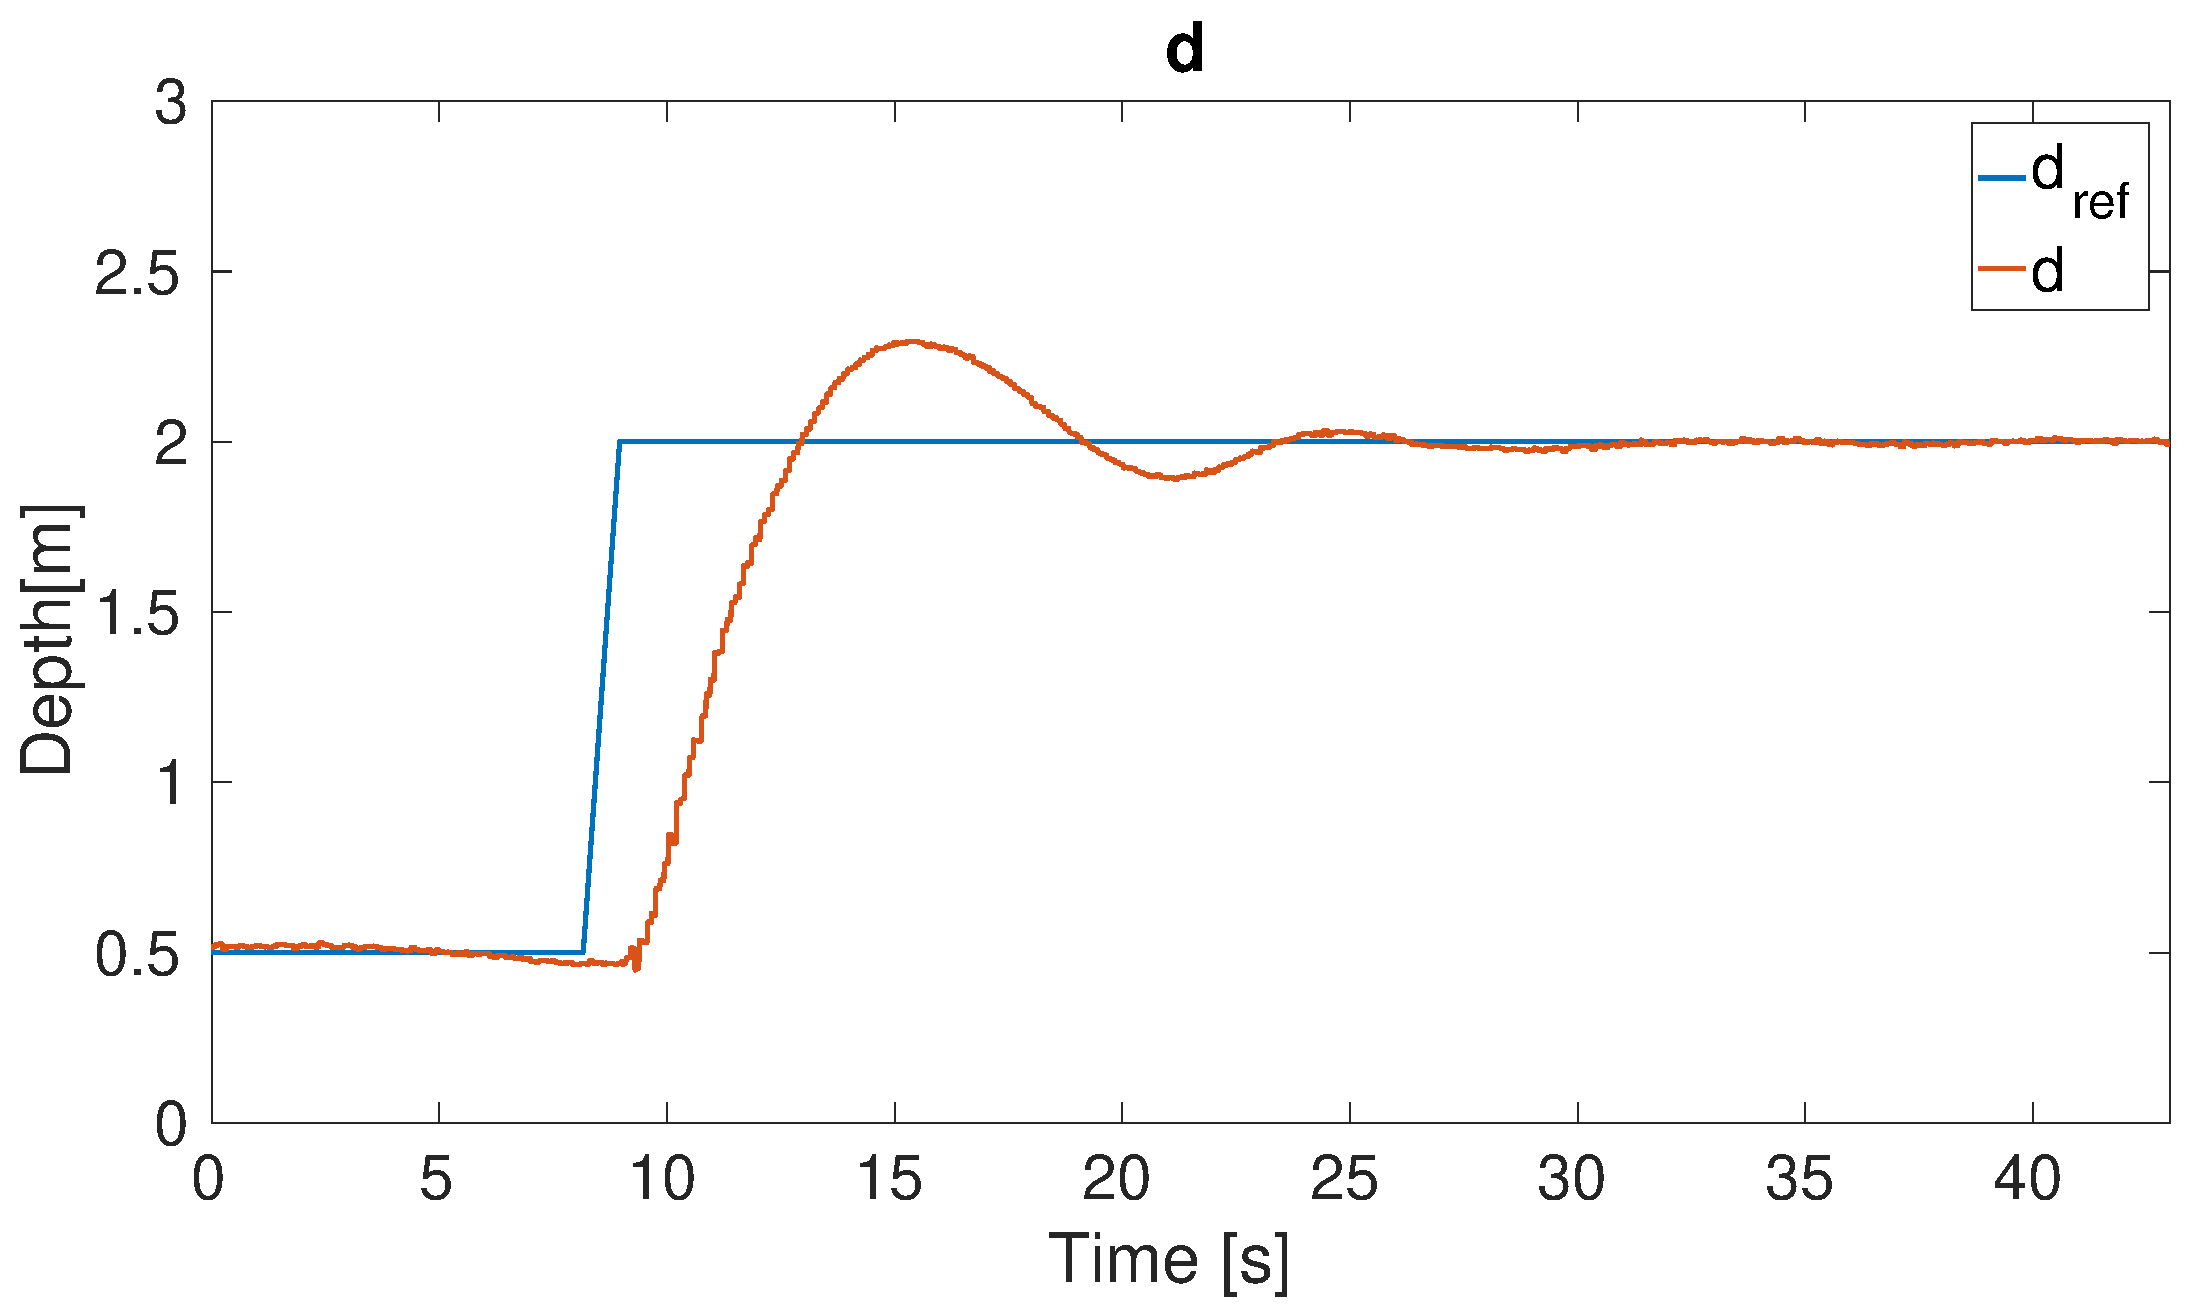
\includegraphics[width=0.4\textwidth]{testConstantD1}}
  \qquad
  \subfloat[][\label{fig:testStepD2} An step was applied to $\zPosition$.]{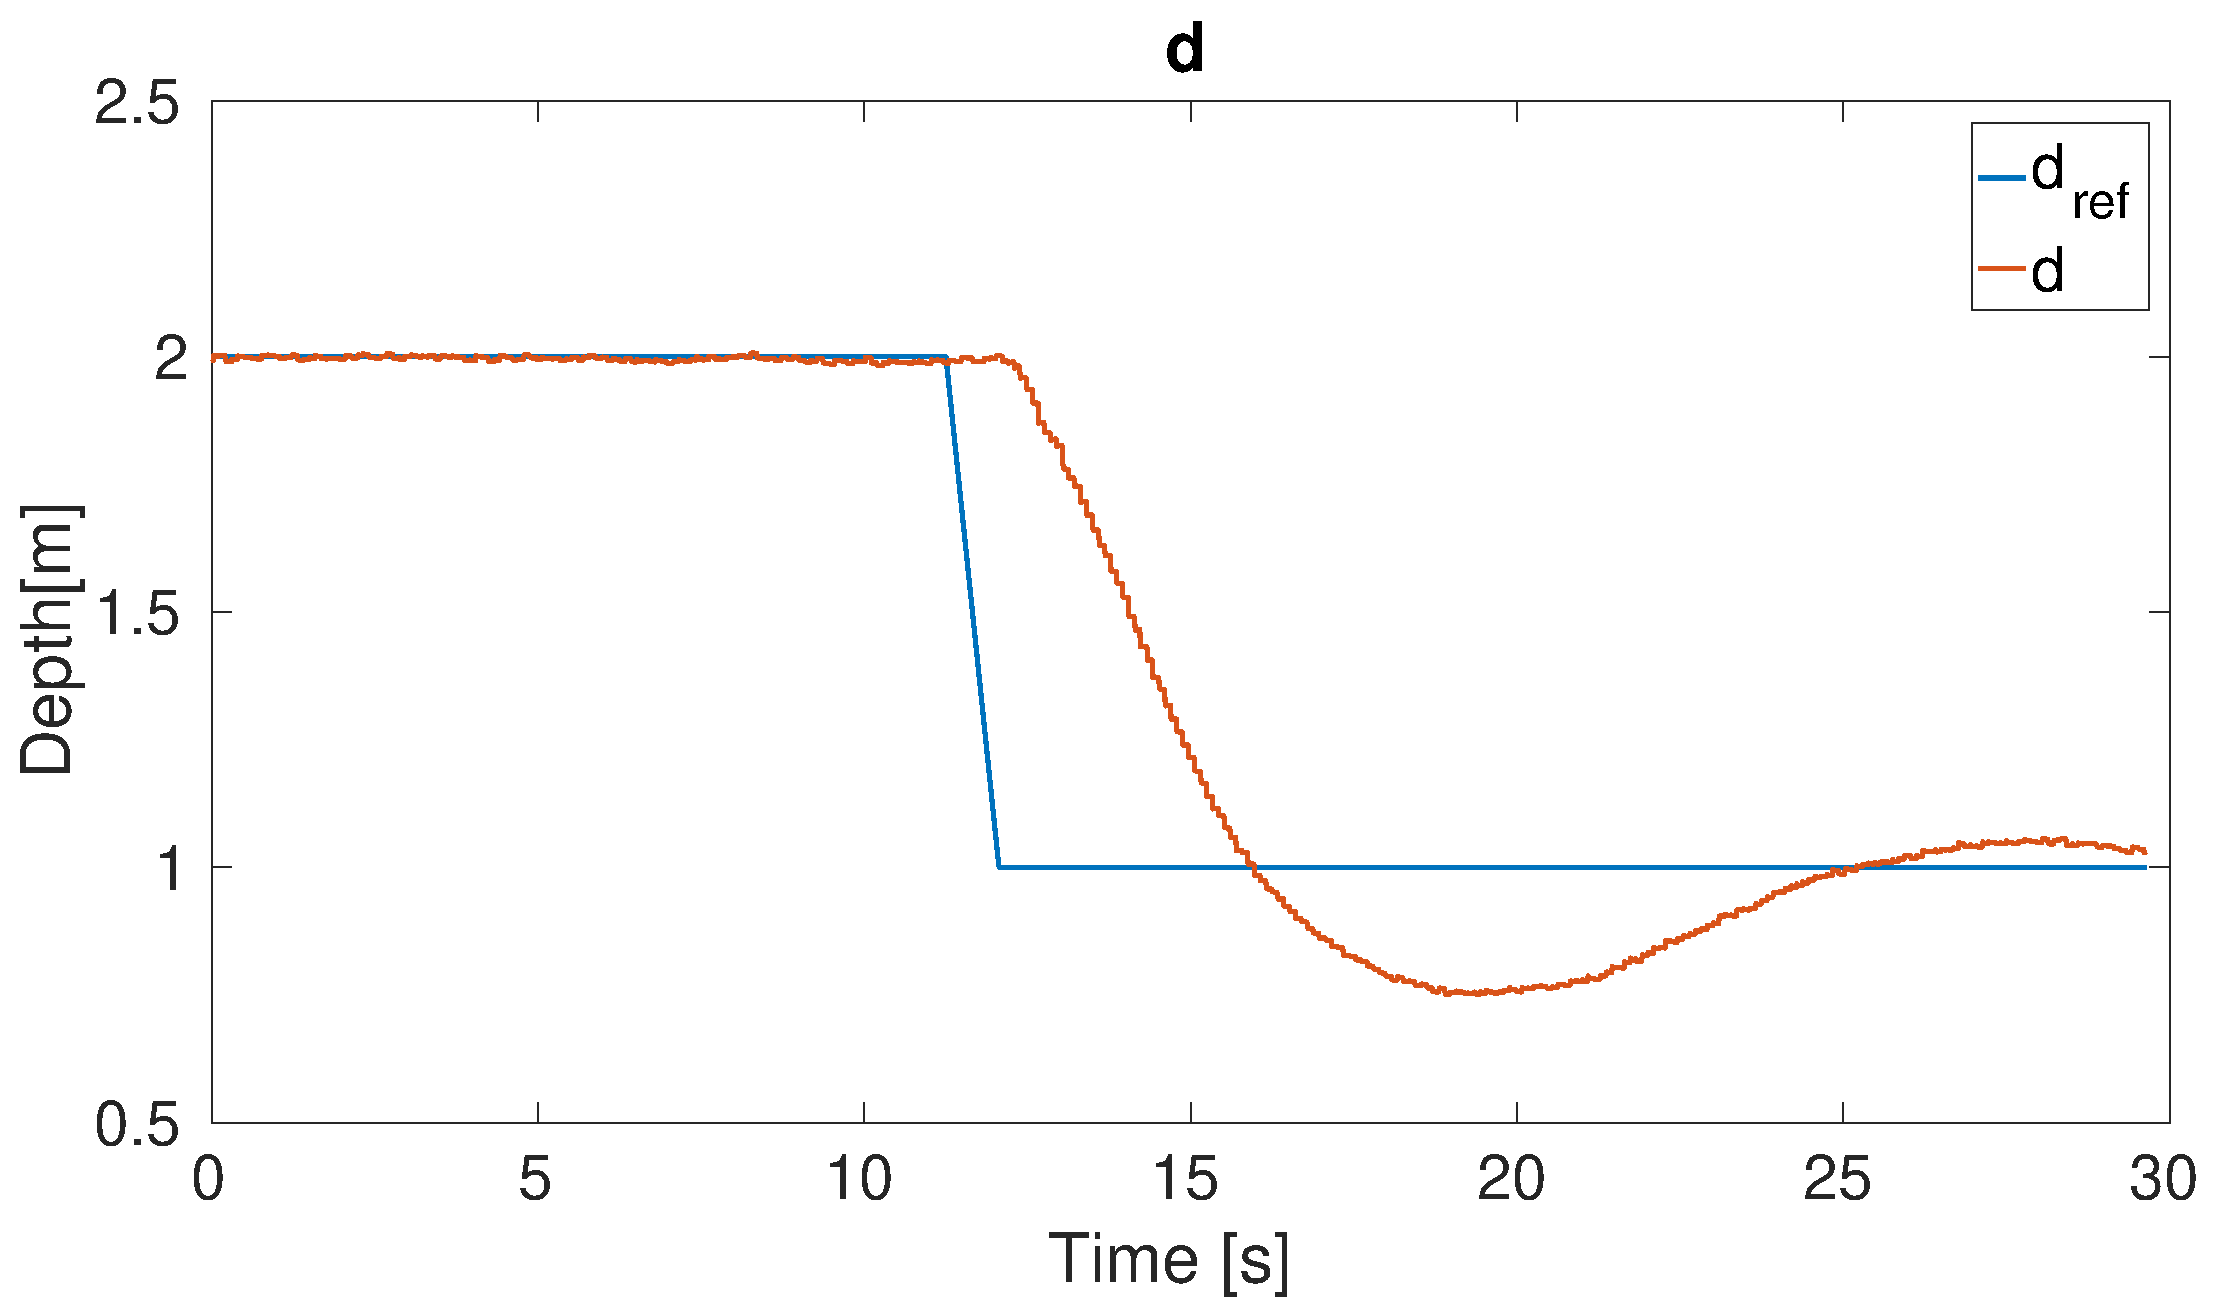
\includegraphics[width=0.4\textwidth]{testConstantD2}}
  \caption{\label{fig:StepD}%
    Steps applied to $\zPosition$. As can be seen there is an slight delay in the response of the controller and overshoots can be seen.}
\end{figure}
\todo[inline]{Fix figures with real results.}
%%%%%%%%%%%%%%%%%%%%%%%%%%%%%%%%%%%%%%%%
\subsection{Simulated Performance}


%%%%%%%%%%%%%%%%%%%%%%%%%%%%%%%%%%%%%%%%
\subsection{Test Performance}
%%%%%%%%%%%%%%%%%%%%%%%%%%%%%%%%%%%%%%%%
\subsection{Conclusions}
